\chapter{Figuras e Resultados}\label{chp:appendice_b}

Partições encontradas pelos modelos melhor ranqueados mencionados no primeiro conjunto de experimentos realizados, encontrado na Seção \ref{sec:ranquemaento}.

\begin{figure}[H]
\centering
\begin{minipage}{.4\textwidth}
  \centering
  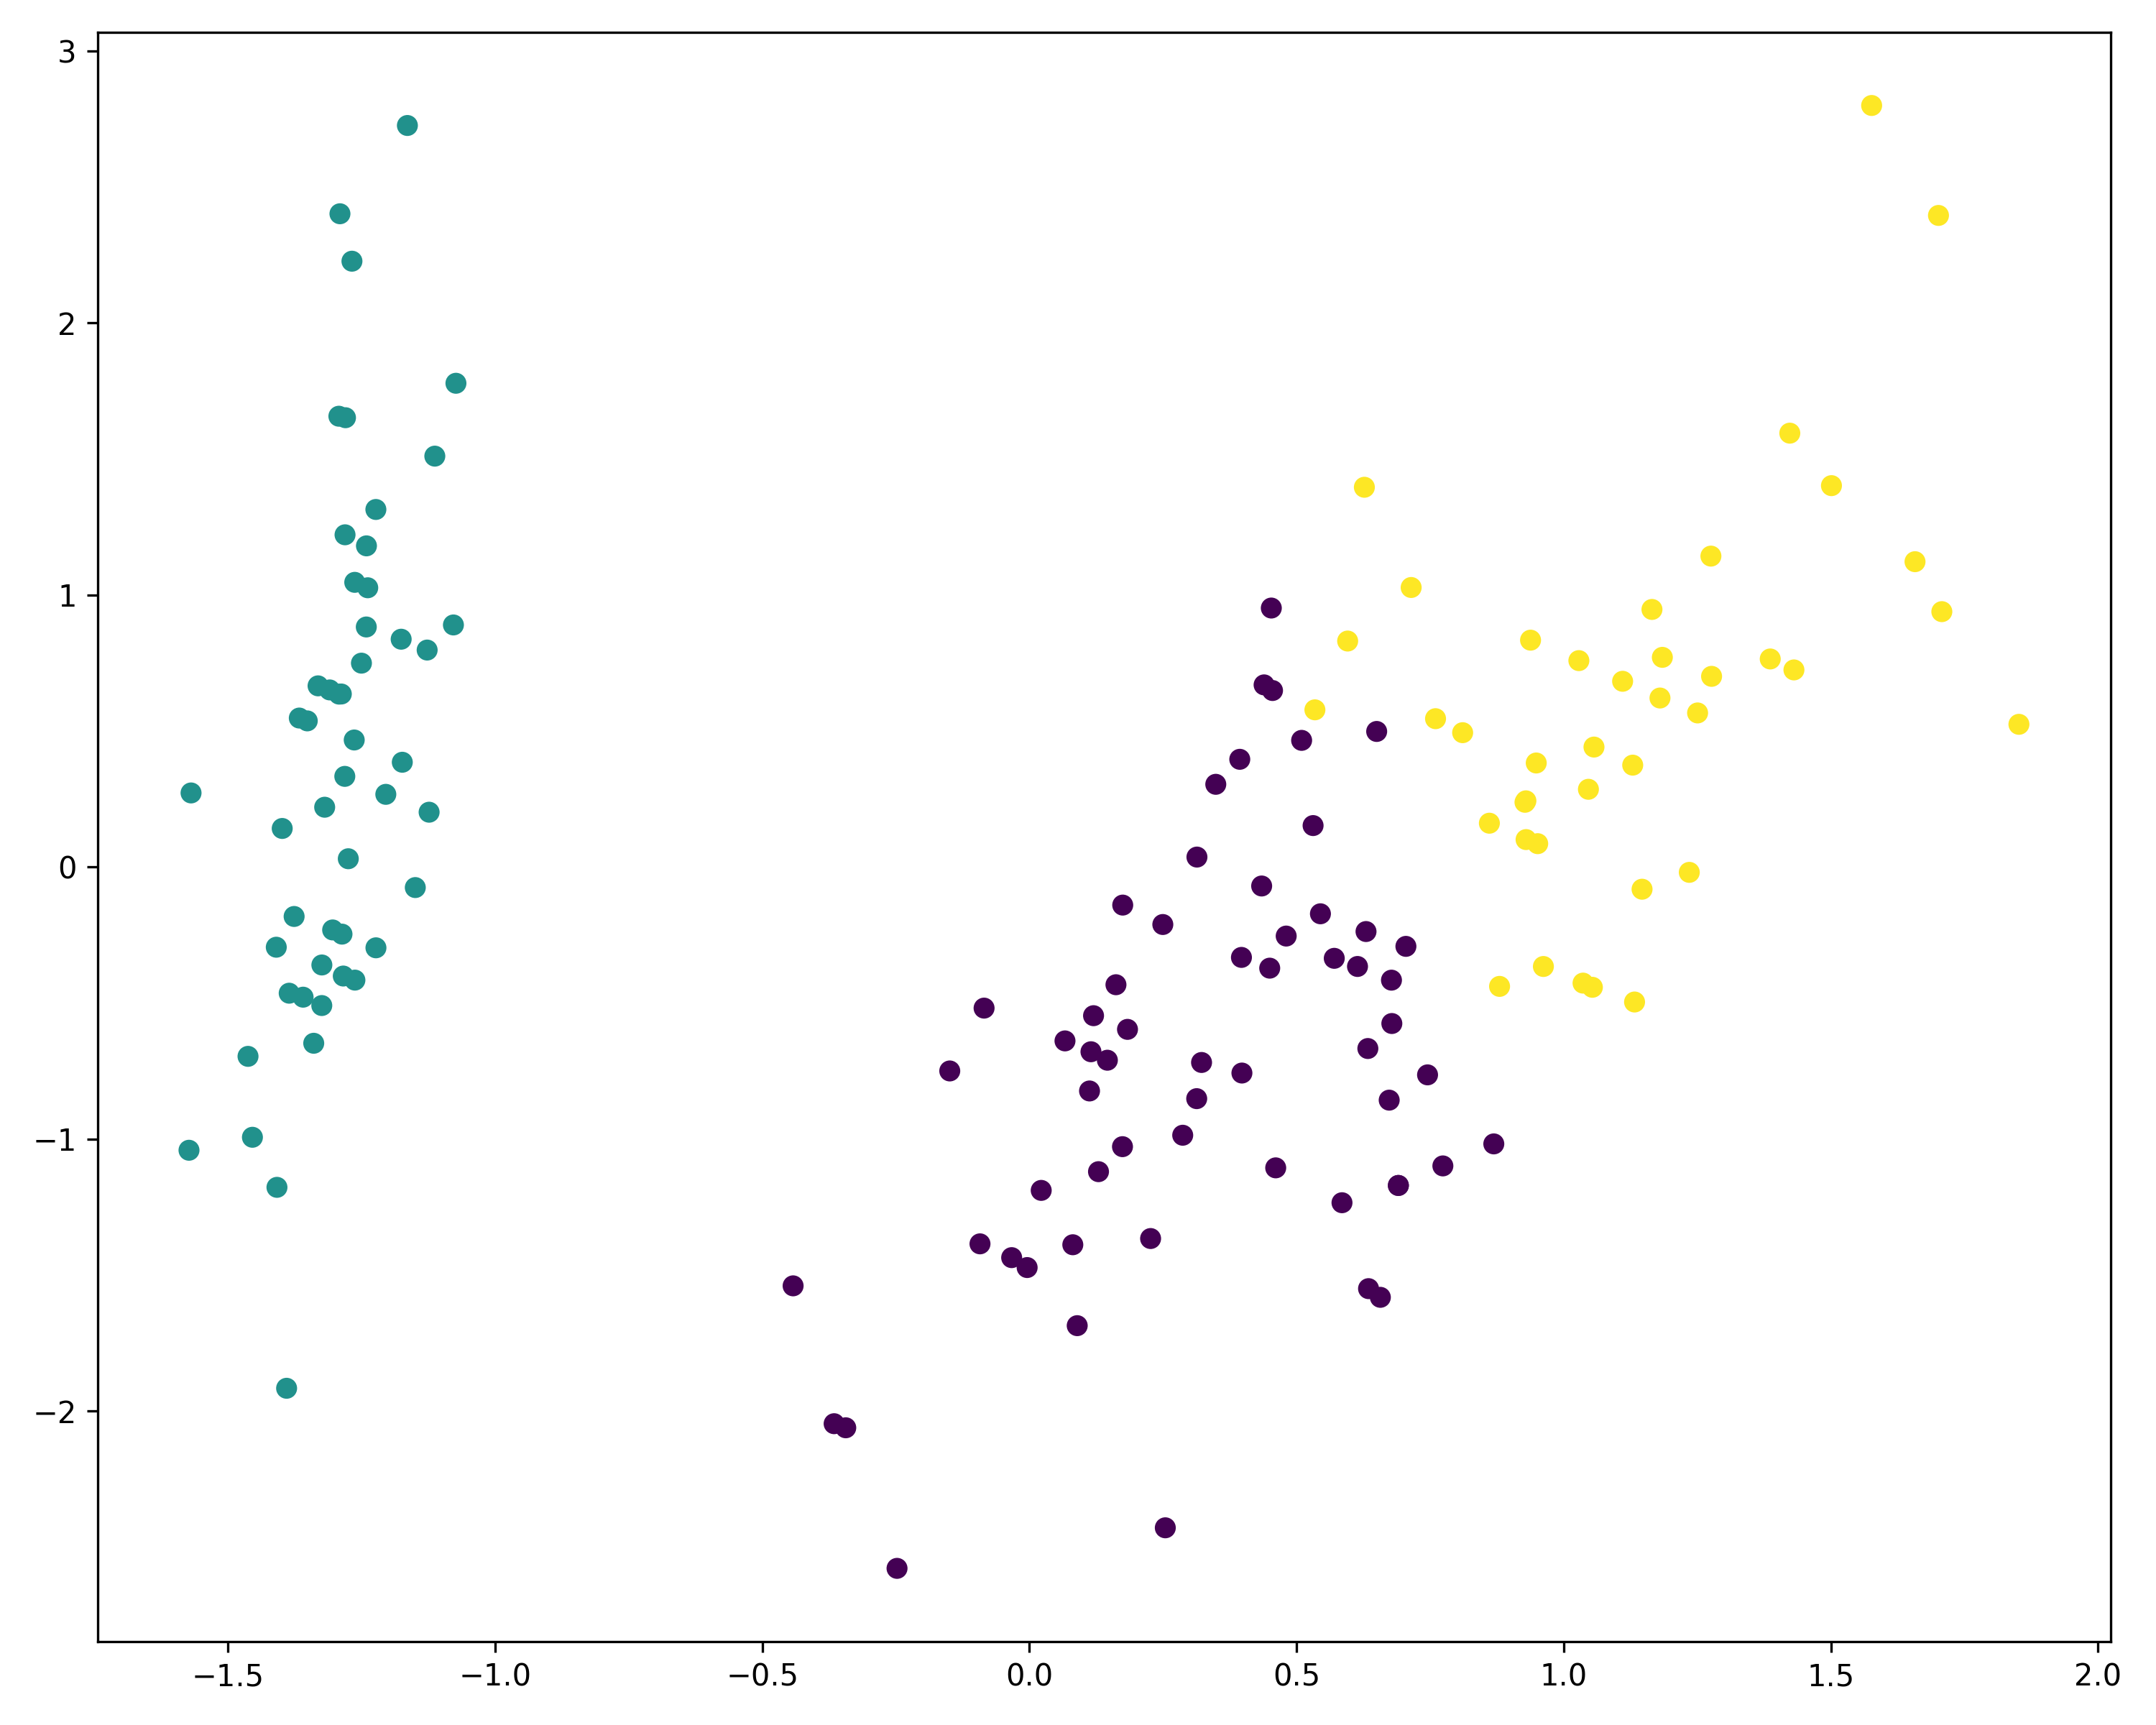
\includegraphics[width=\linewidth]{images/claire/random_n0_iris_kernel_kmeans_n_clusters_3_kernel_gak_random_state_0.png}
\end{minipage}%
\vspace{.02\textwidth}%
\begin{minipage}{.4\textwidth}
  \centering
  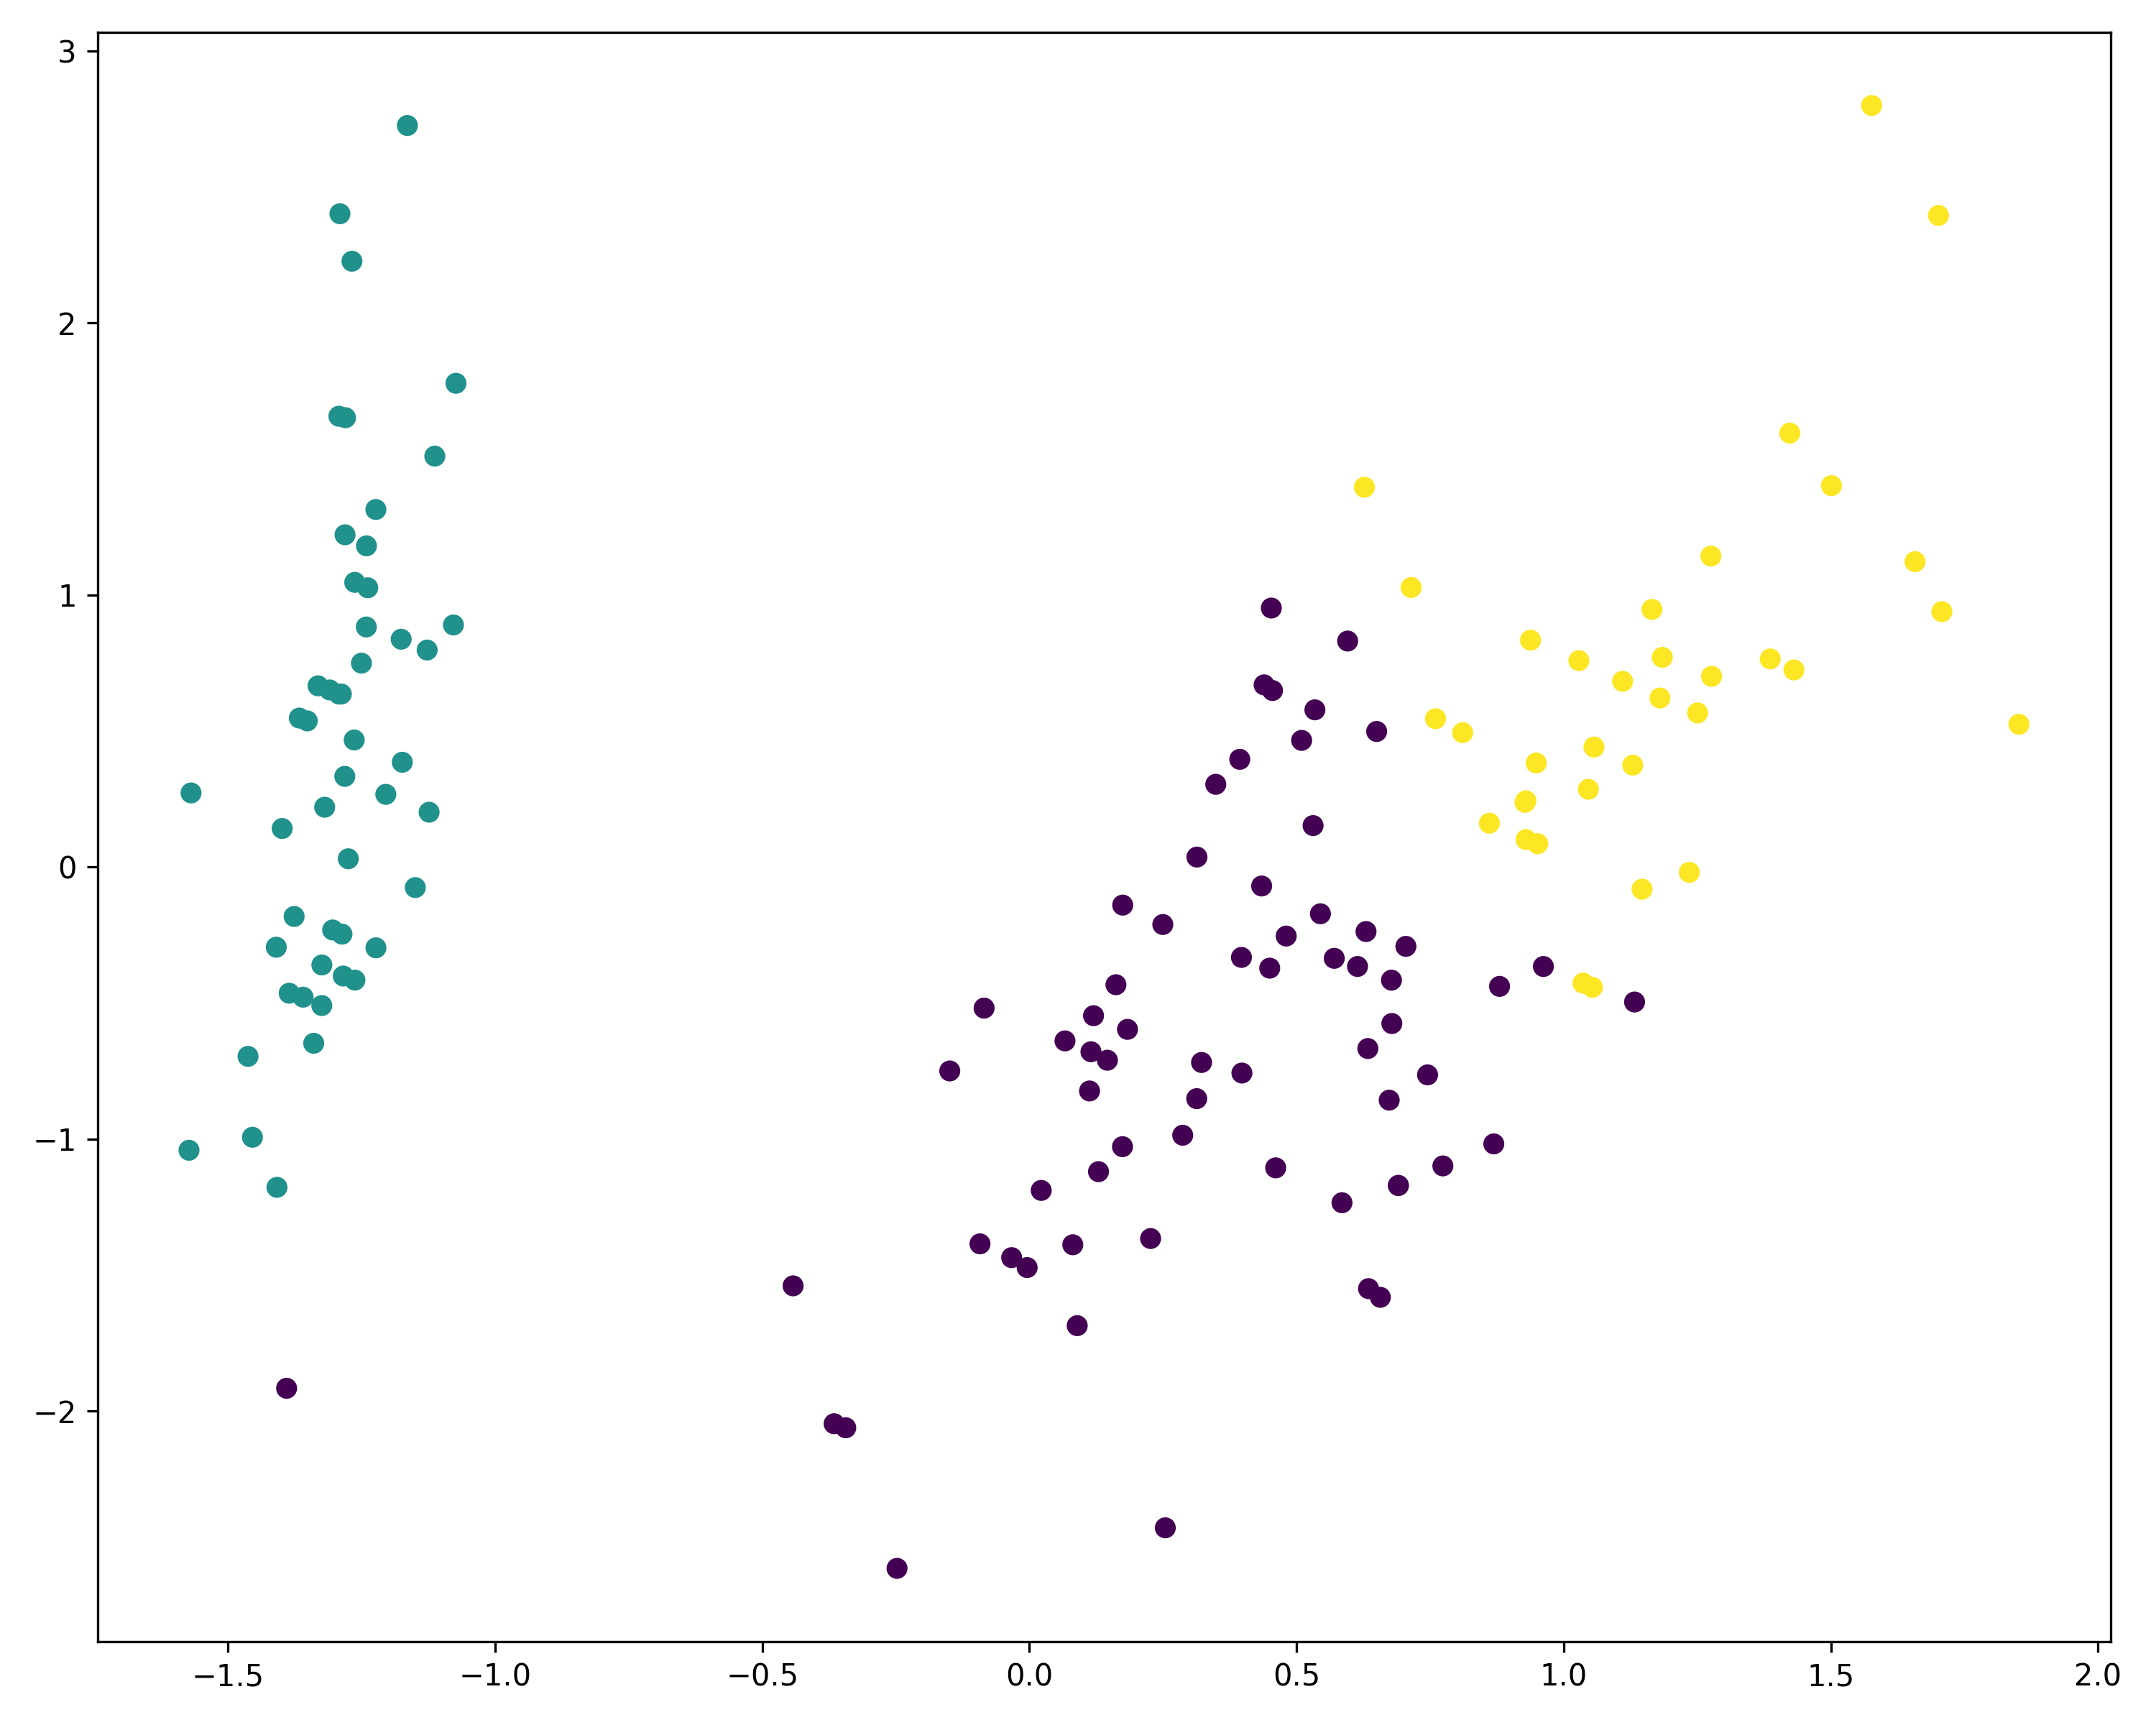
\includegraphics[width=\linewidth]{images/claire/random_n0_iris_spectral_clustering_n_clusters_3_eigen_solver_arpack_affinity_nearest_neighbors.png}
\end{minipage}
\caption{Melhores partições encontradas por Kernel K-means ($K = 3$) e Spectral Clustering ($K = 3$), para o conjunto de dados Iris.}
\end{figure}


\begin{figure}[H]
\centering
\begin{minipage}{0.45\textwidth}
  \centering
  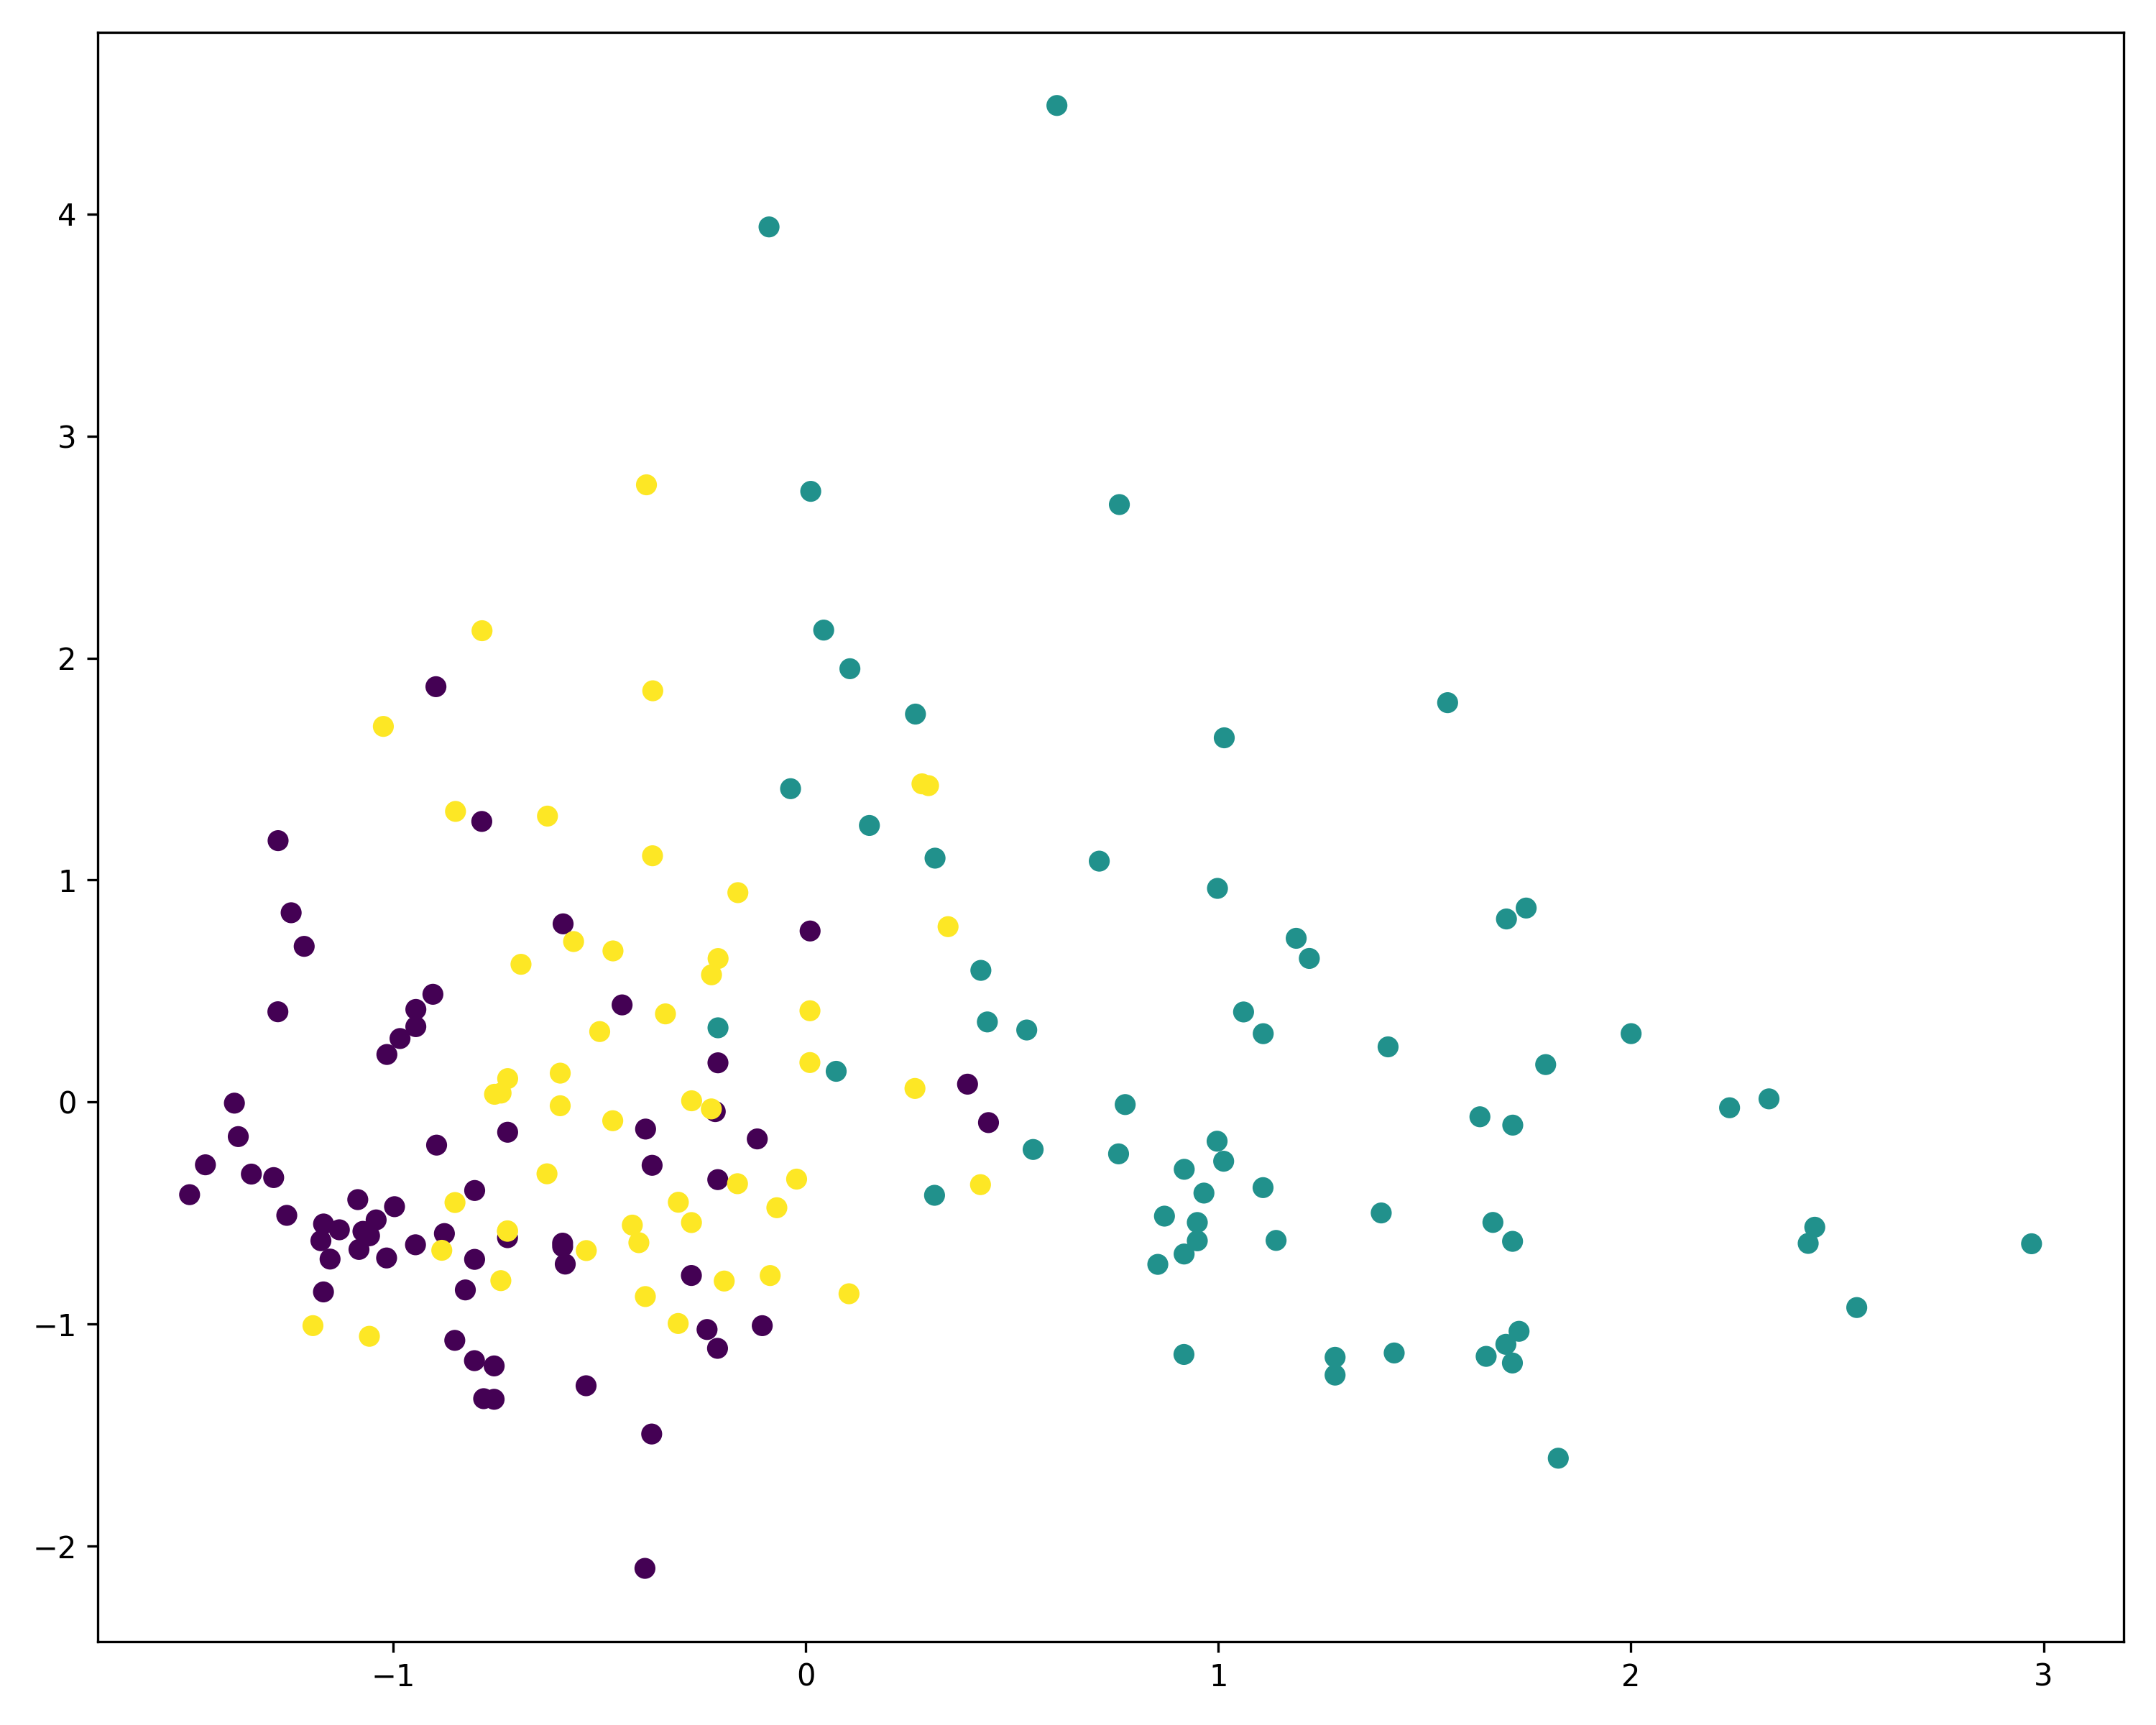
\includegraphics[width=\linewidth]{images/claire/random_n0_wine_spectral_clustering_n_clusters_3_eigen_solver_arpack_affinity_nearest_neighbors.png}
\end{minipage}
\caption{Melhor partição encontrada por Spectral Clustering ($K = 3$), para o conjunto de dados Wine.}


\end{figure}


\begin{figure}
\centering
\begin{minipage}{.4\textwidth}
  \centering
  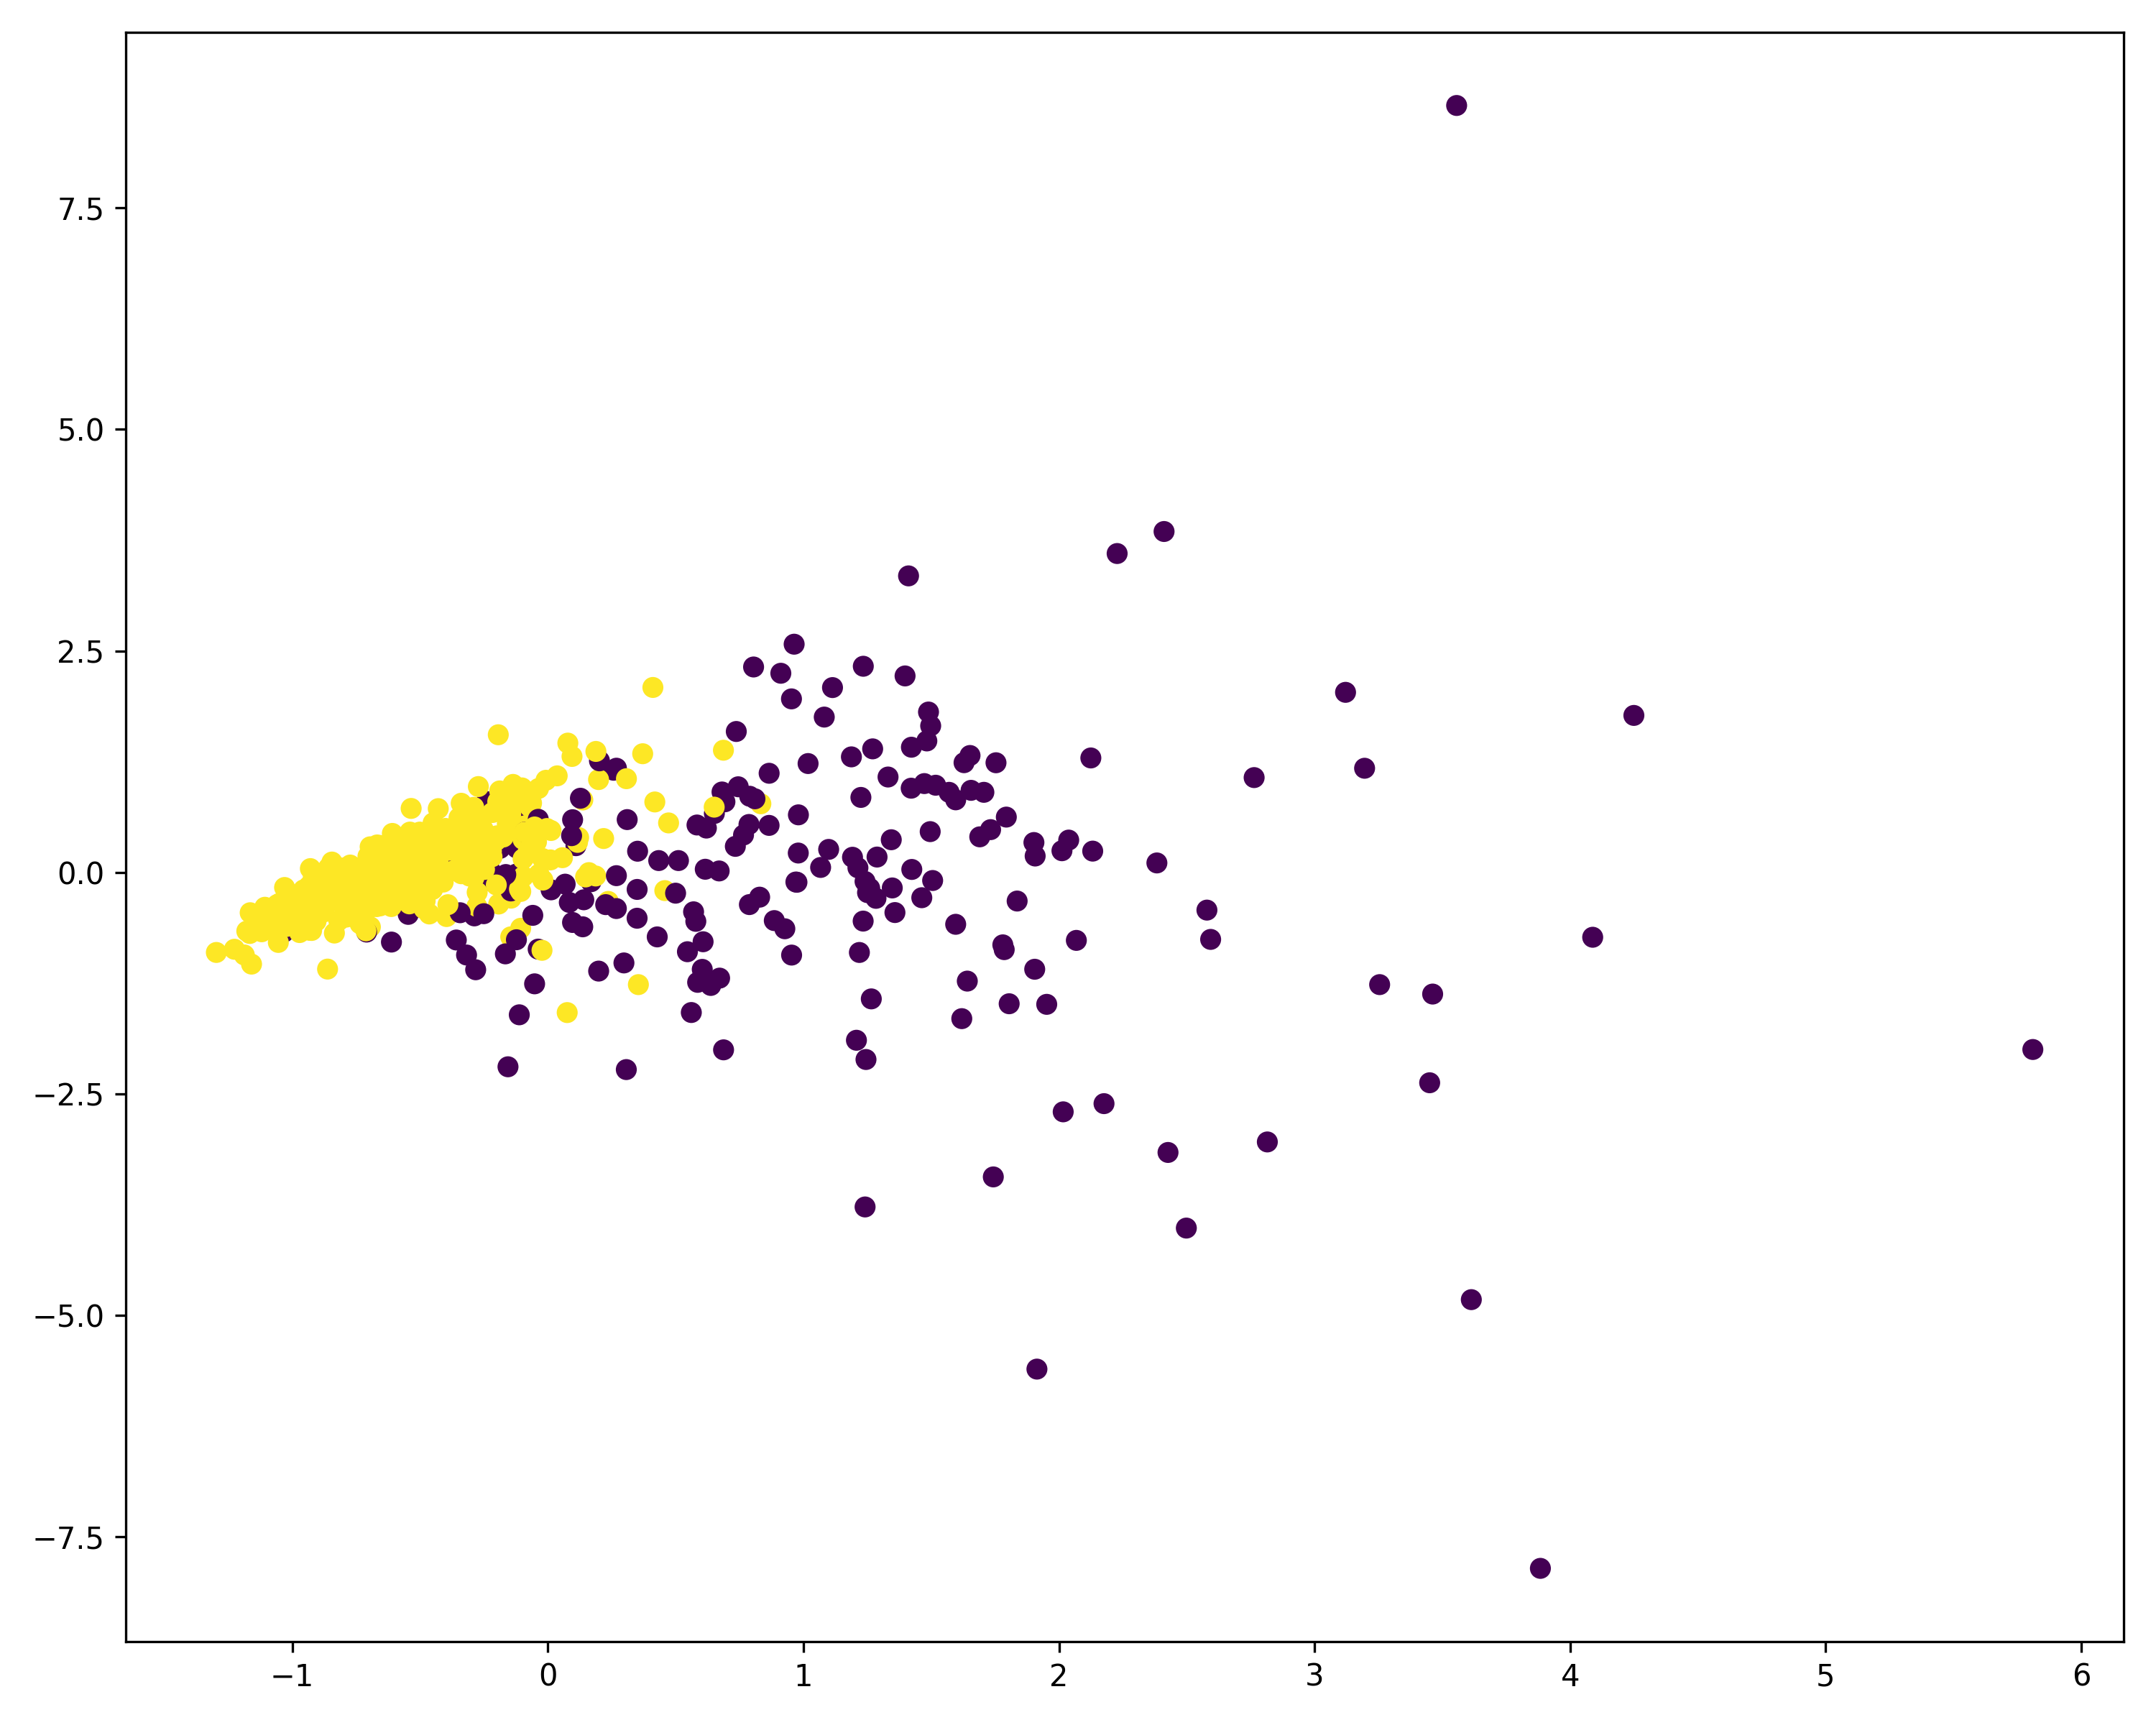
\includegraphics[width=\linewidth]{images/claire/random_n0_breast_cancer_spectral_clustering_n_clusters_2_eigen_solver_arpack_affinity_nearest_neighbors.png}
\caption{Melhor partição encontrada por Spectral Clustering ($K = 2$), para o conjunto de dados Breast Cancer.}

\end{minipage}%
\hspace{.05\textwidth} % Espaço entre as figuras
\begin{minipage}{.4\textwidth}
  \centering
  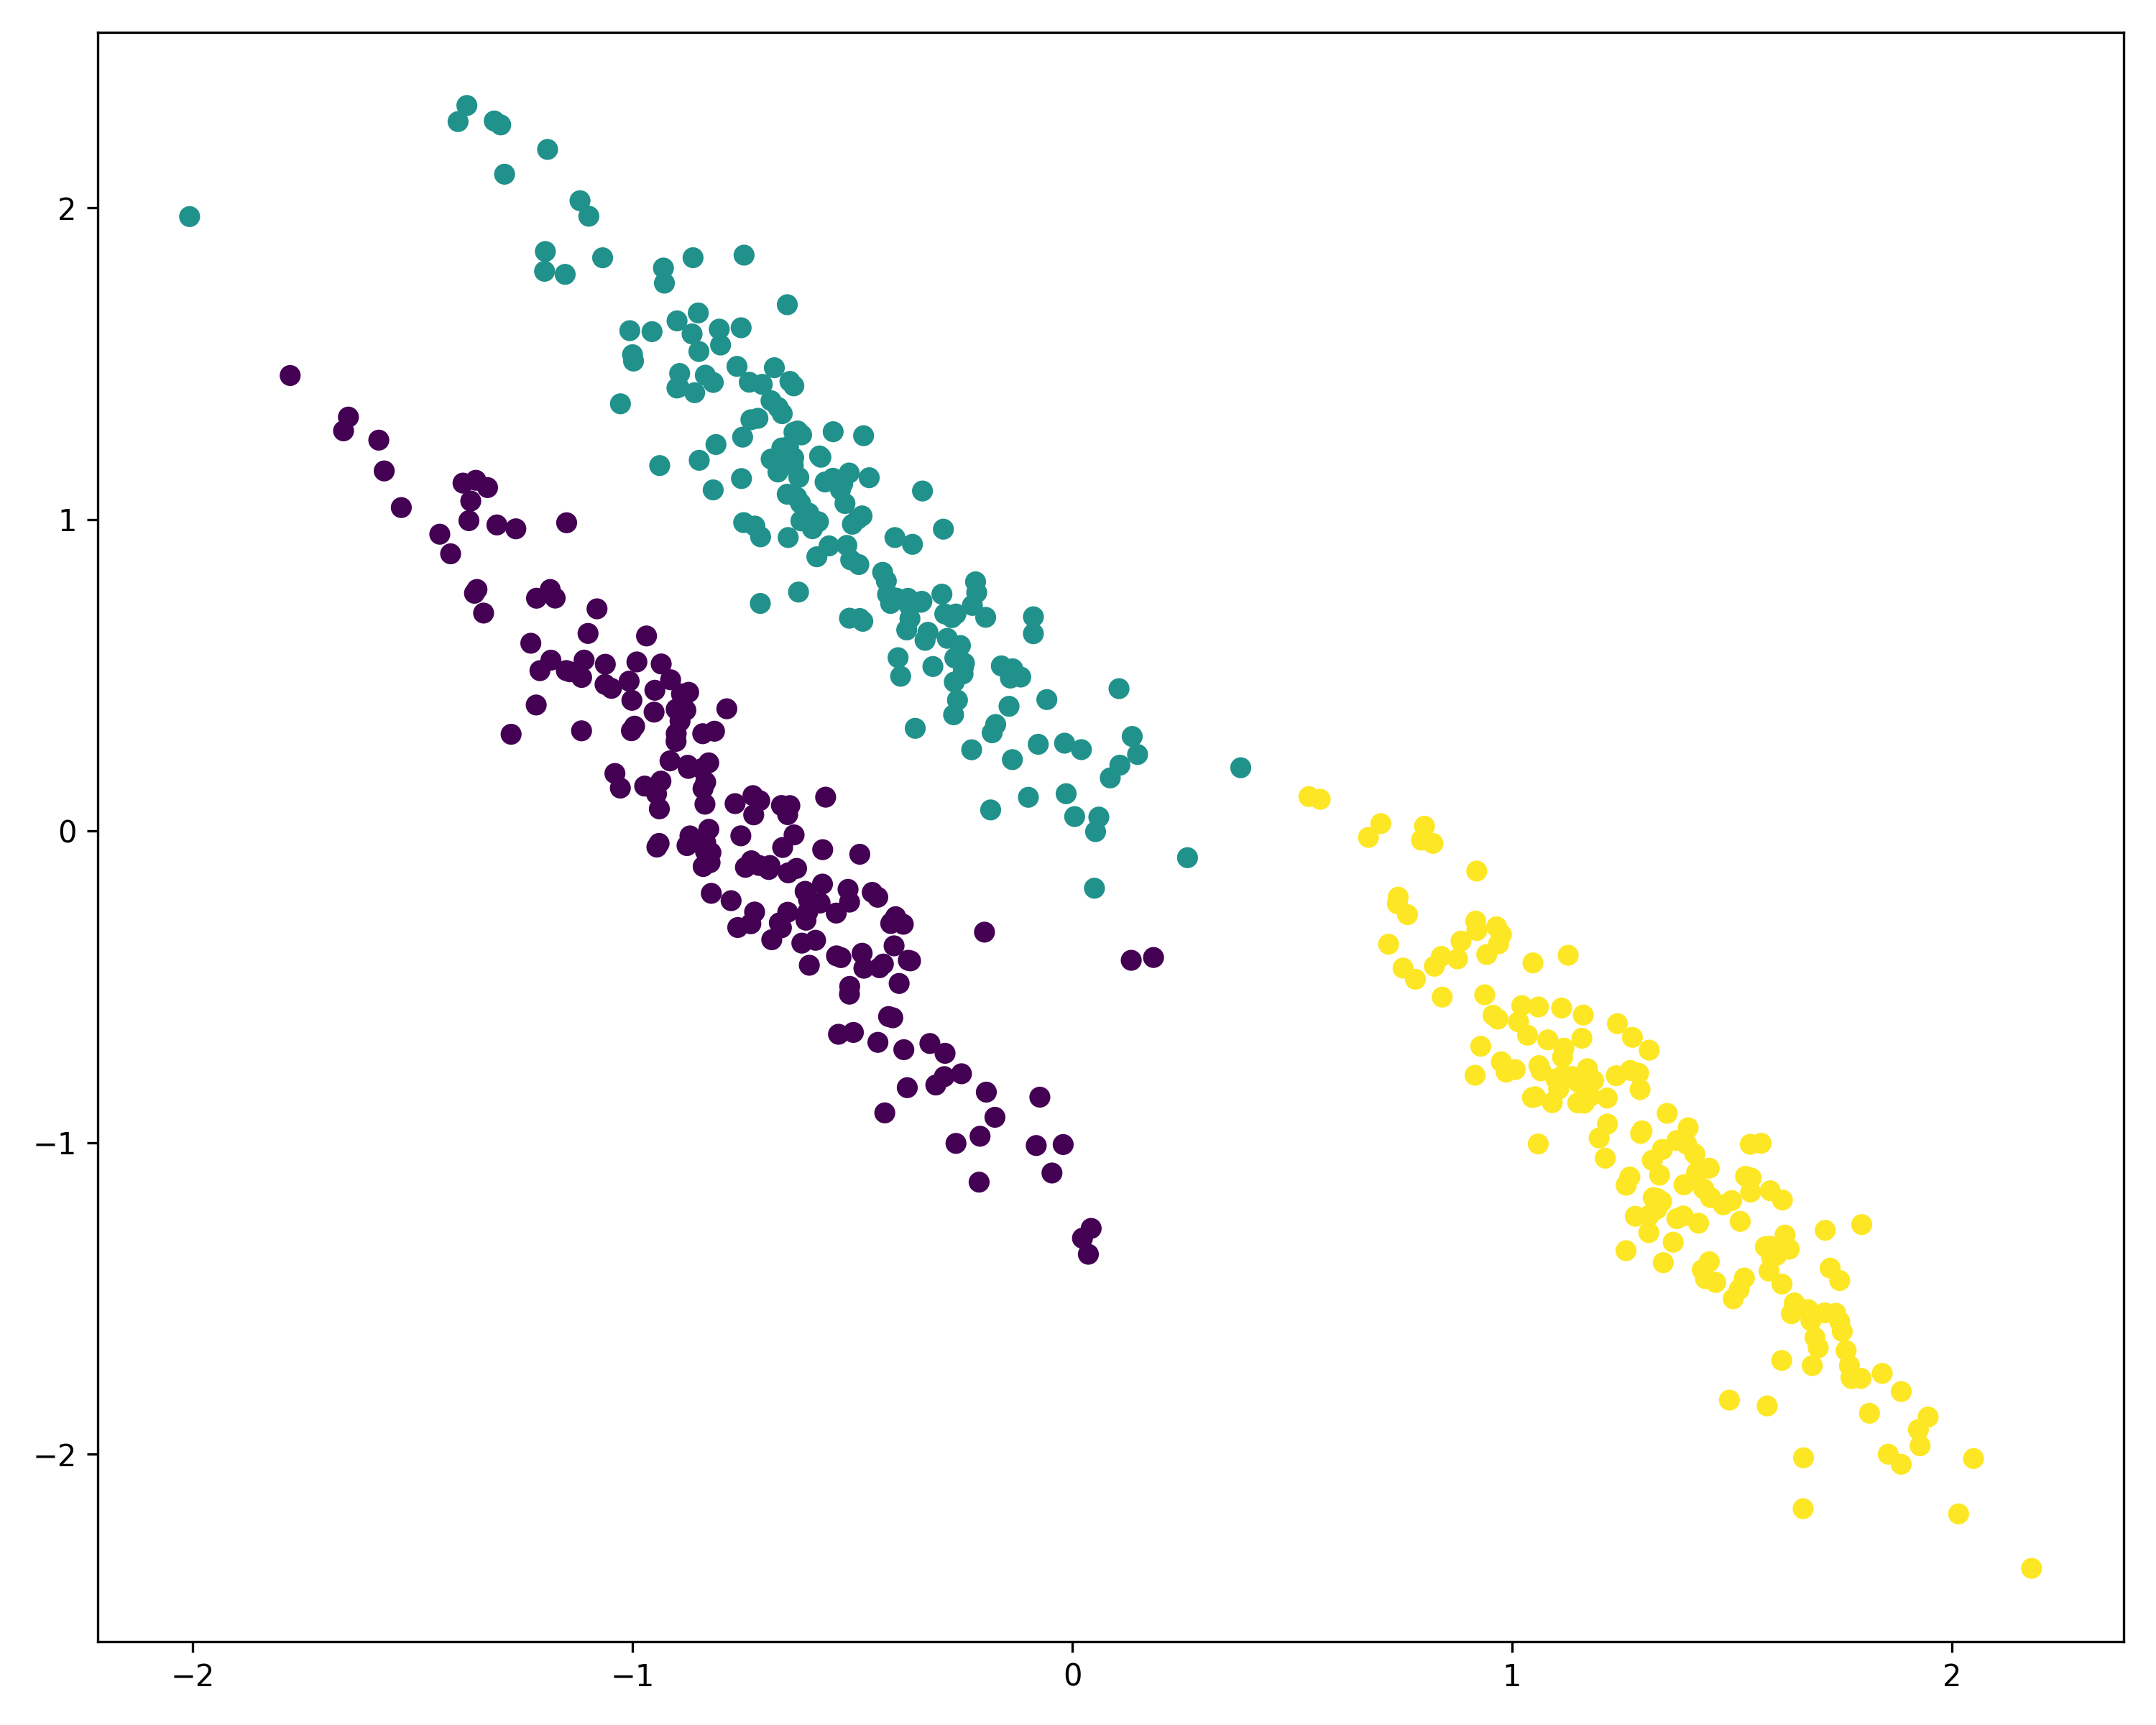
\includegraphics[width=\linewidth]{images/claire/random_n0_aniso_spectral_clustering_n_clusters_3_eigen_solver_arpack_affinity_nearest_neighbors.png}
\caption{A melhor partição foi encontrada por Spectral Clustering ($K = 3$), para o conjunto de dados Aniso.}

\end{minipage}
\end{figure}

\begin{figure}
\centering
\begin{minipage}{.35\textwidth}
  \centering
  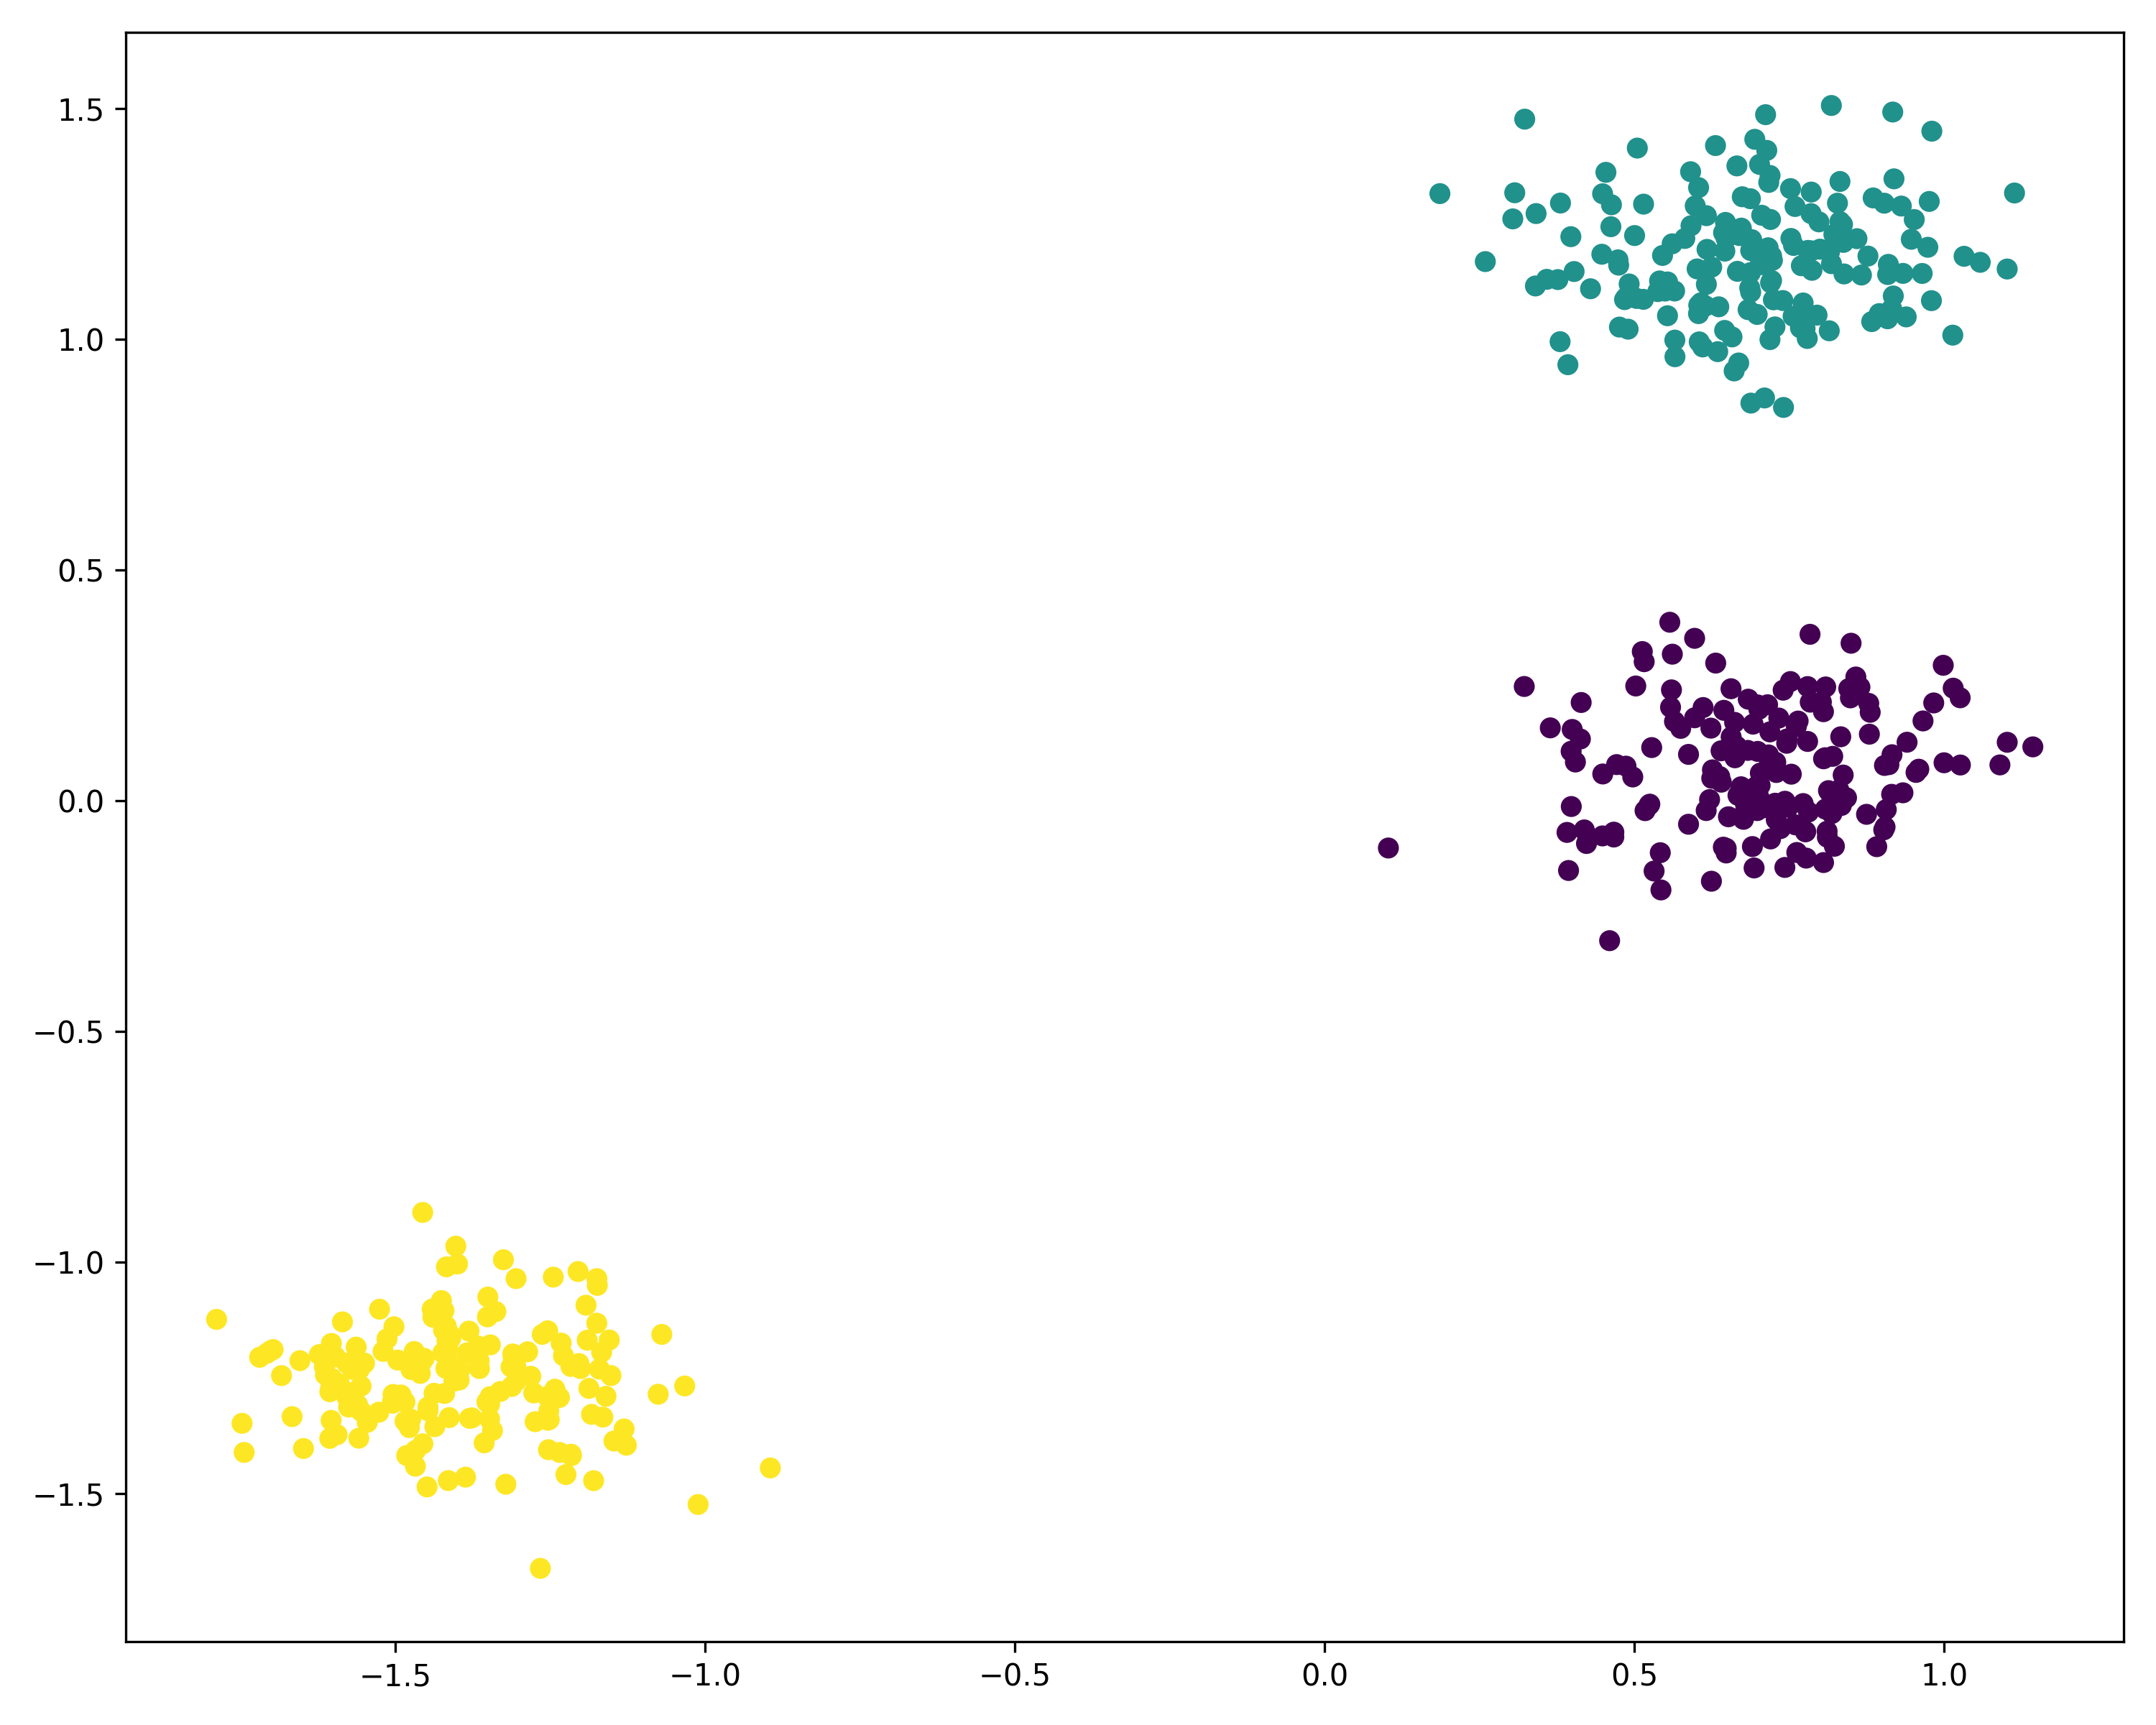
\includegraphics[width=\linewidth]{images/claire/random_n0_blobs_mean_shift_.png}
\end{minipage}%
\hspace{0.02cm}
\begin{minipage}{.35\textwidth}
  \centering
  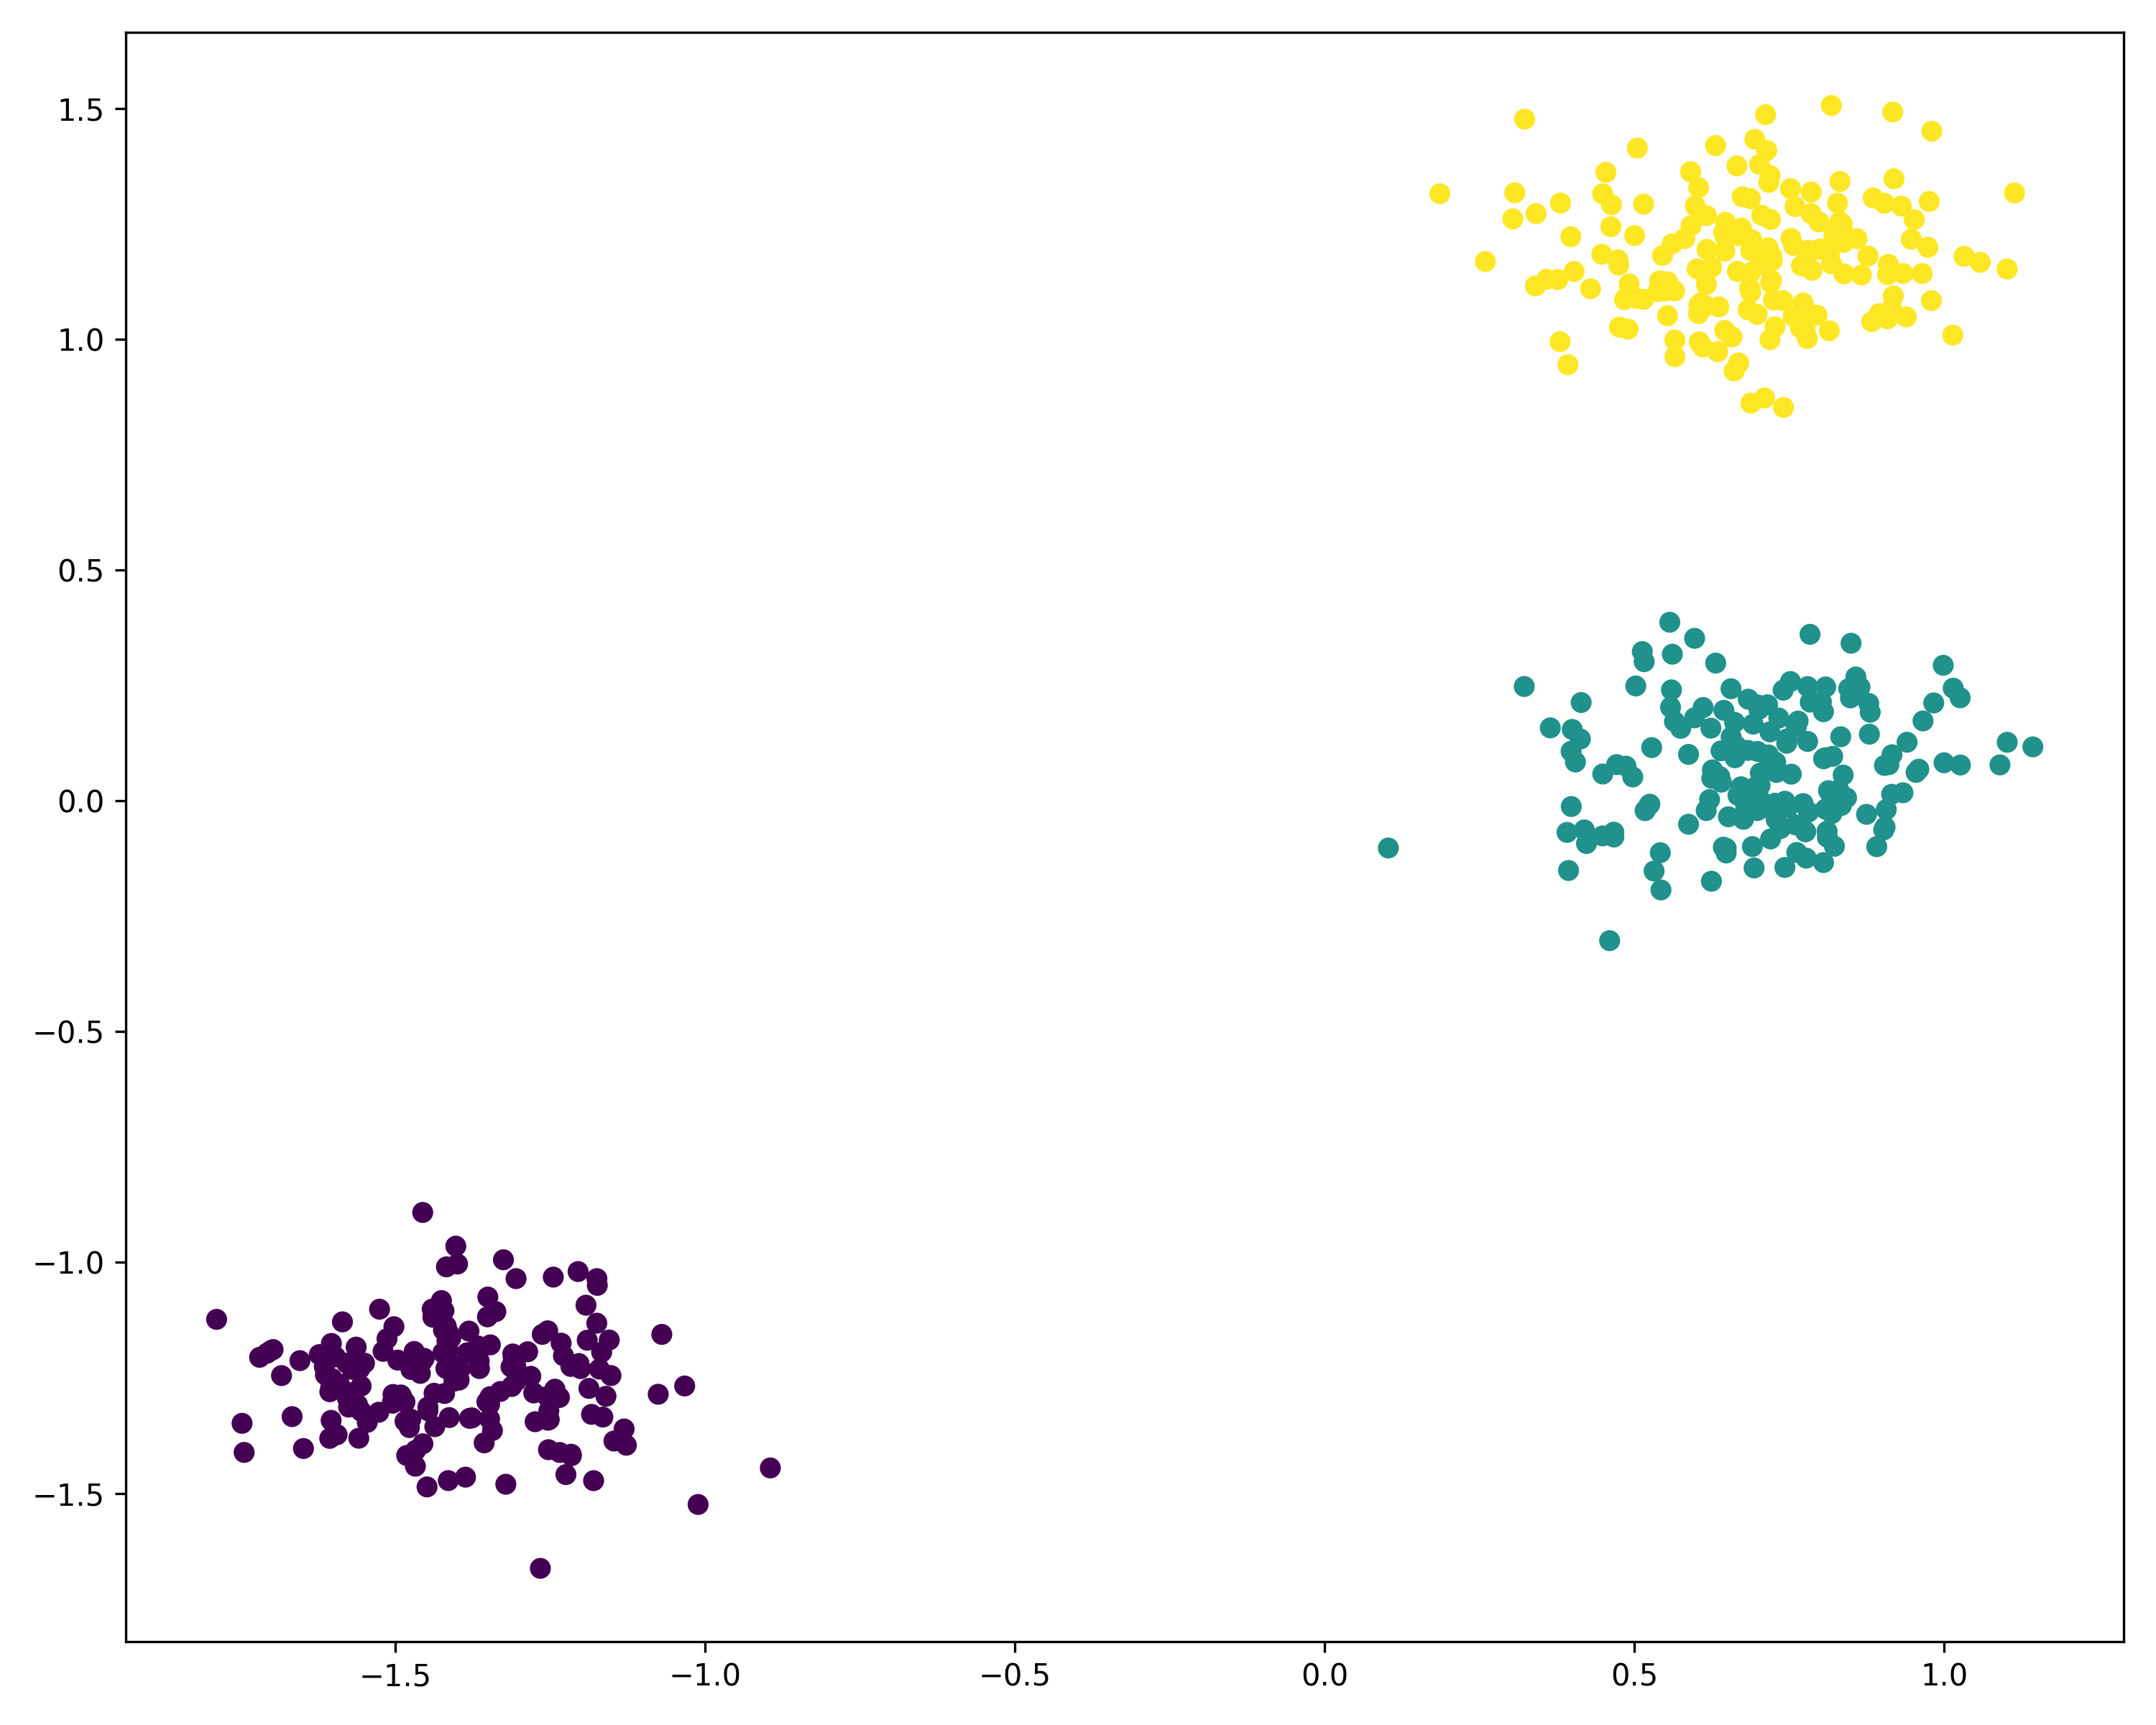
\includegraphics[width=\linewidth]{images/claire/random_n0_blobs_optics_min_samples_7_xi_0_1_min_cluster_size_0_2.png}
\end{minipage}
\vspace{0.02cm}
\begin{minipage}{.35\textwidth}
  \centering
  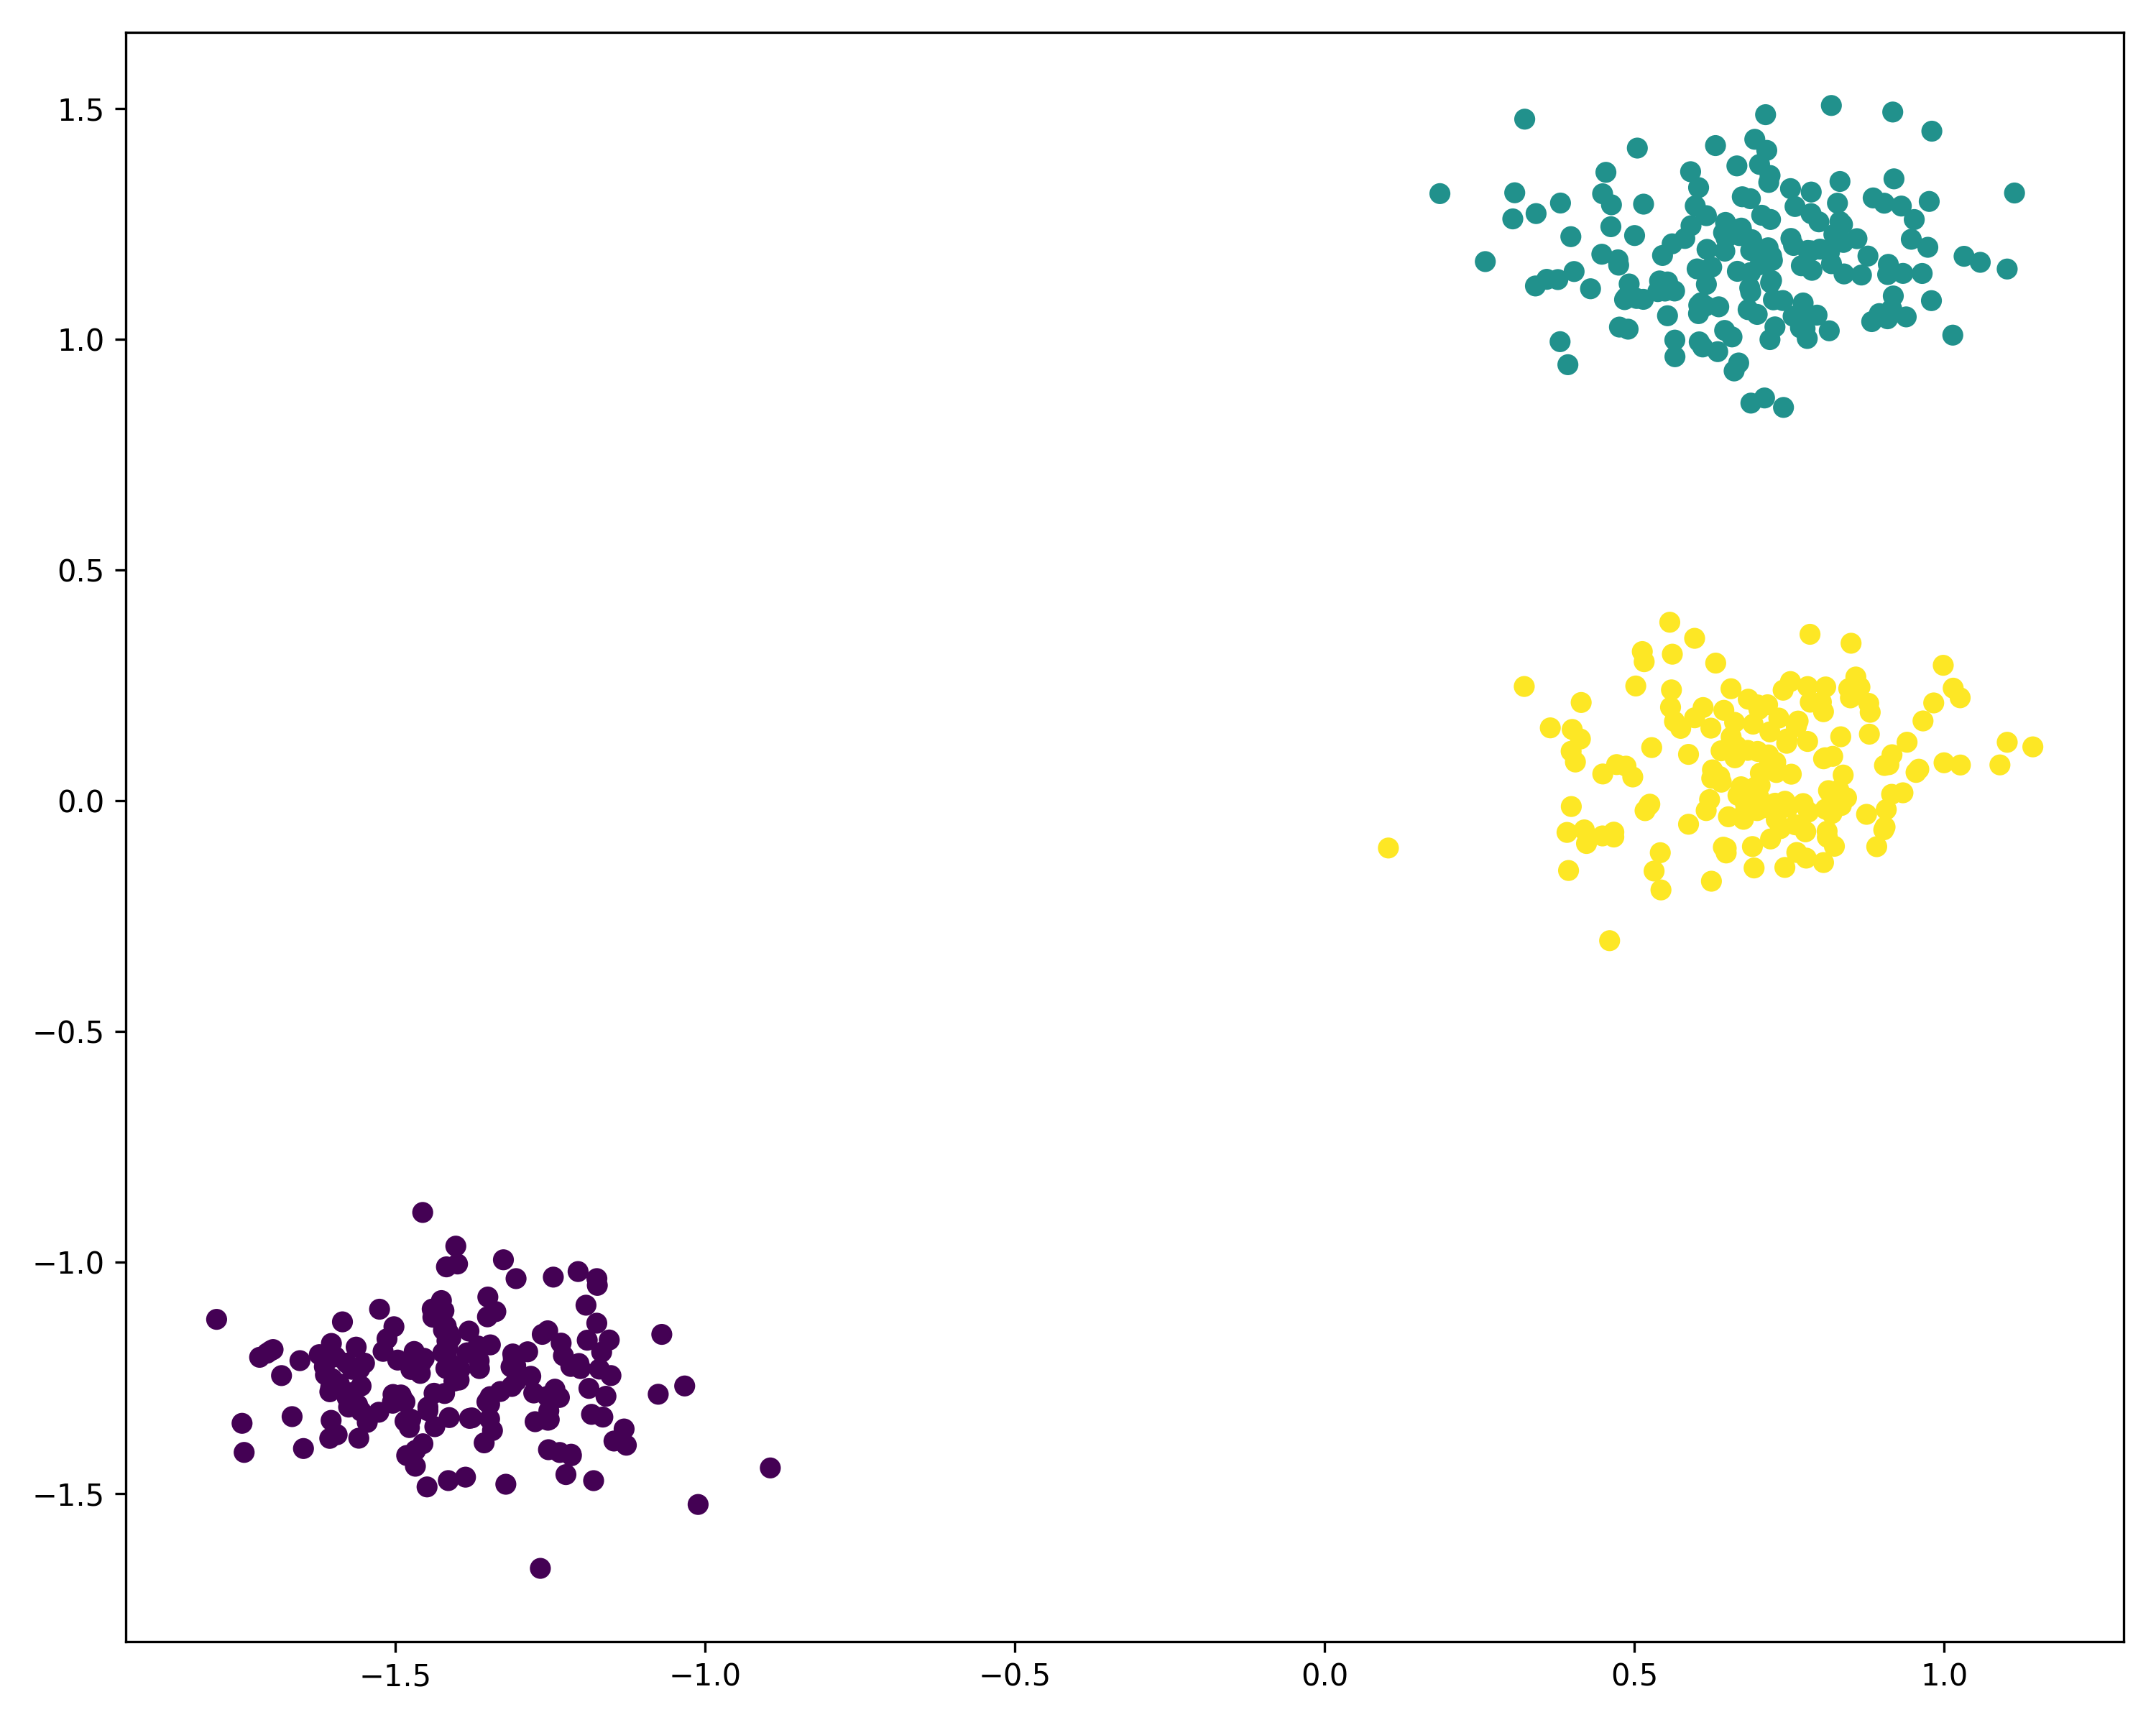
\includegraphics[width=\linewidth]{images/claire/random_n0_blobs_dbscan_eps_0_3_min_samples_2.png}

\end{minipage}%
\hspace{0.02cm}
\begin{minipage}{.35\textwidth}
  \centering
  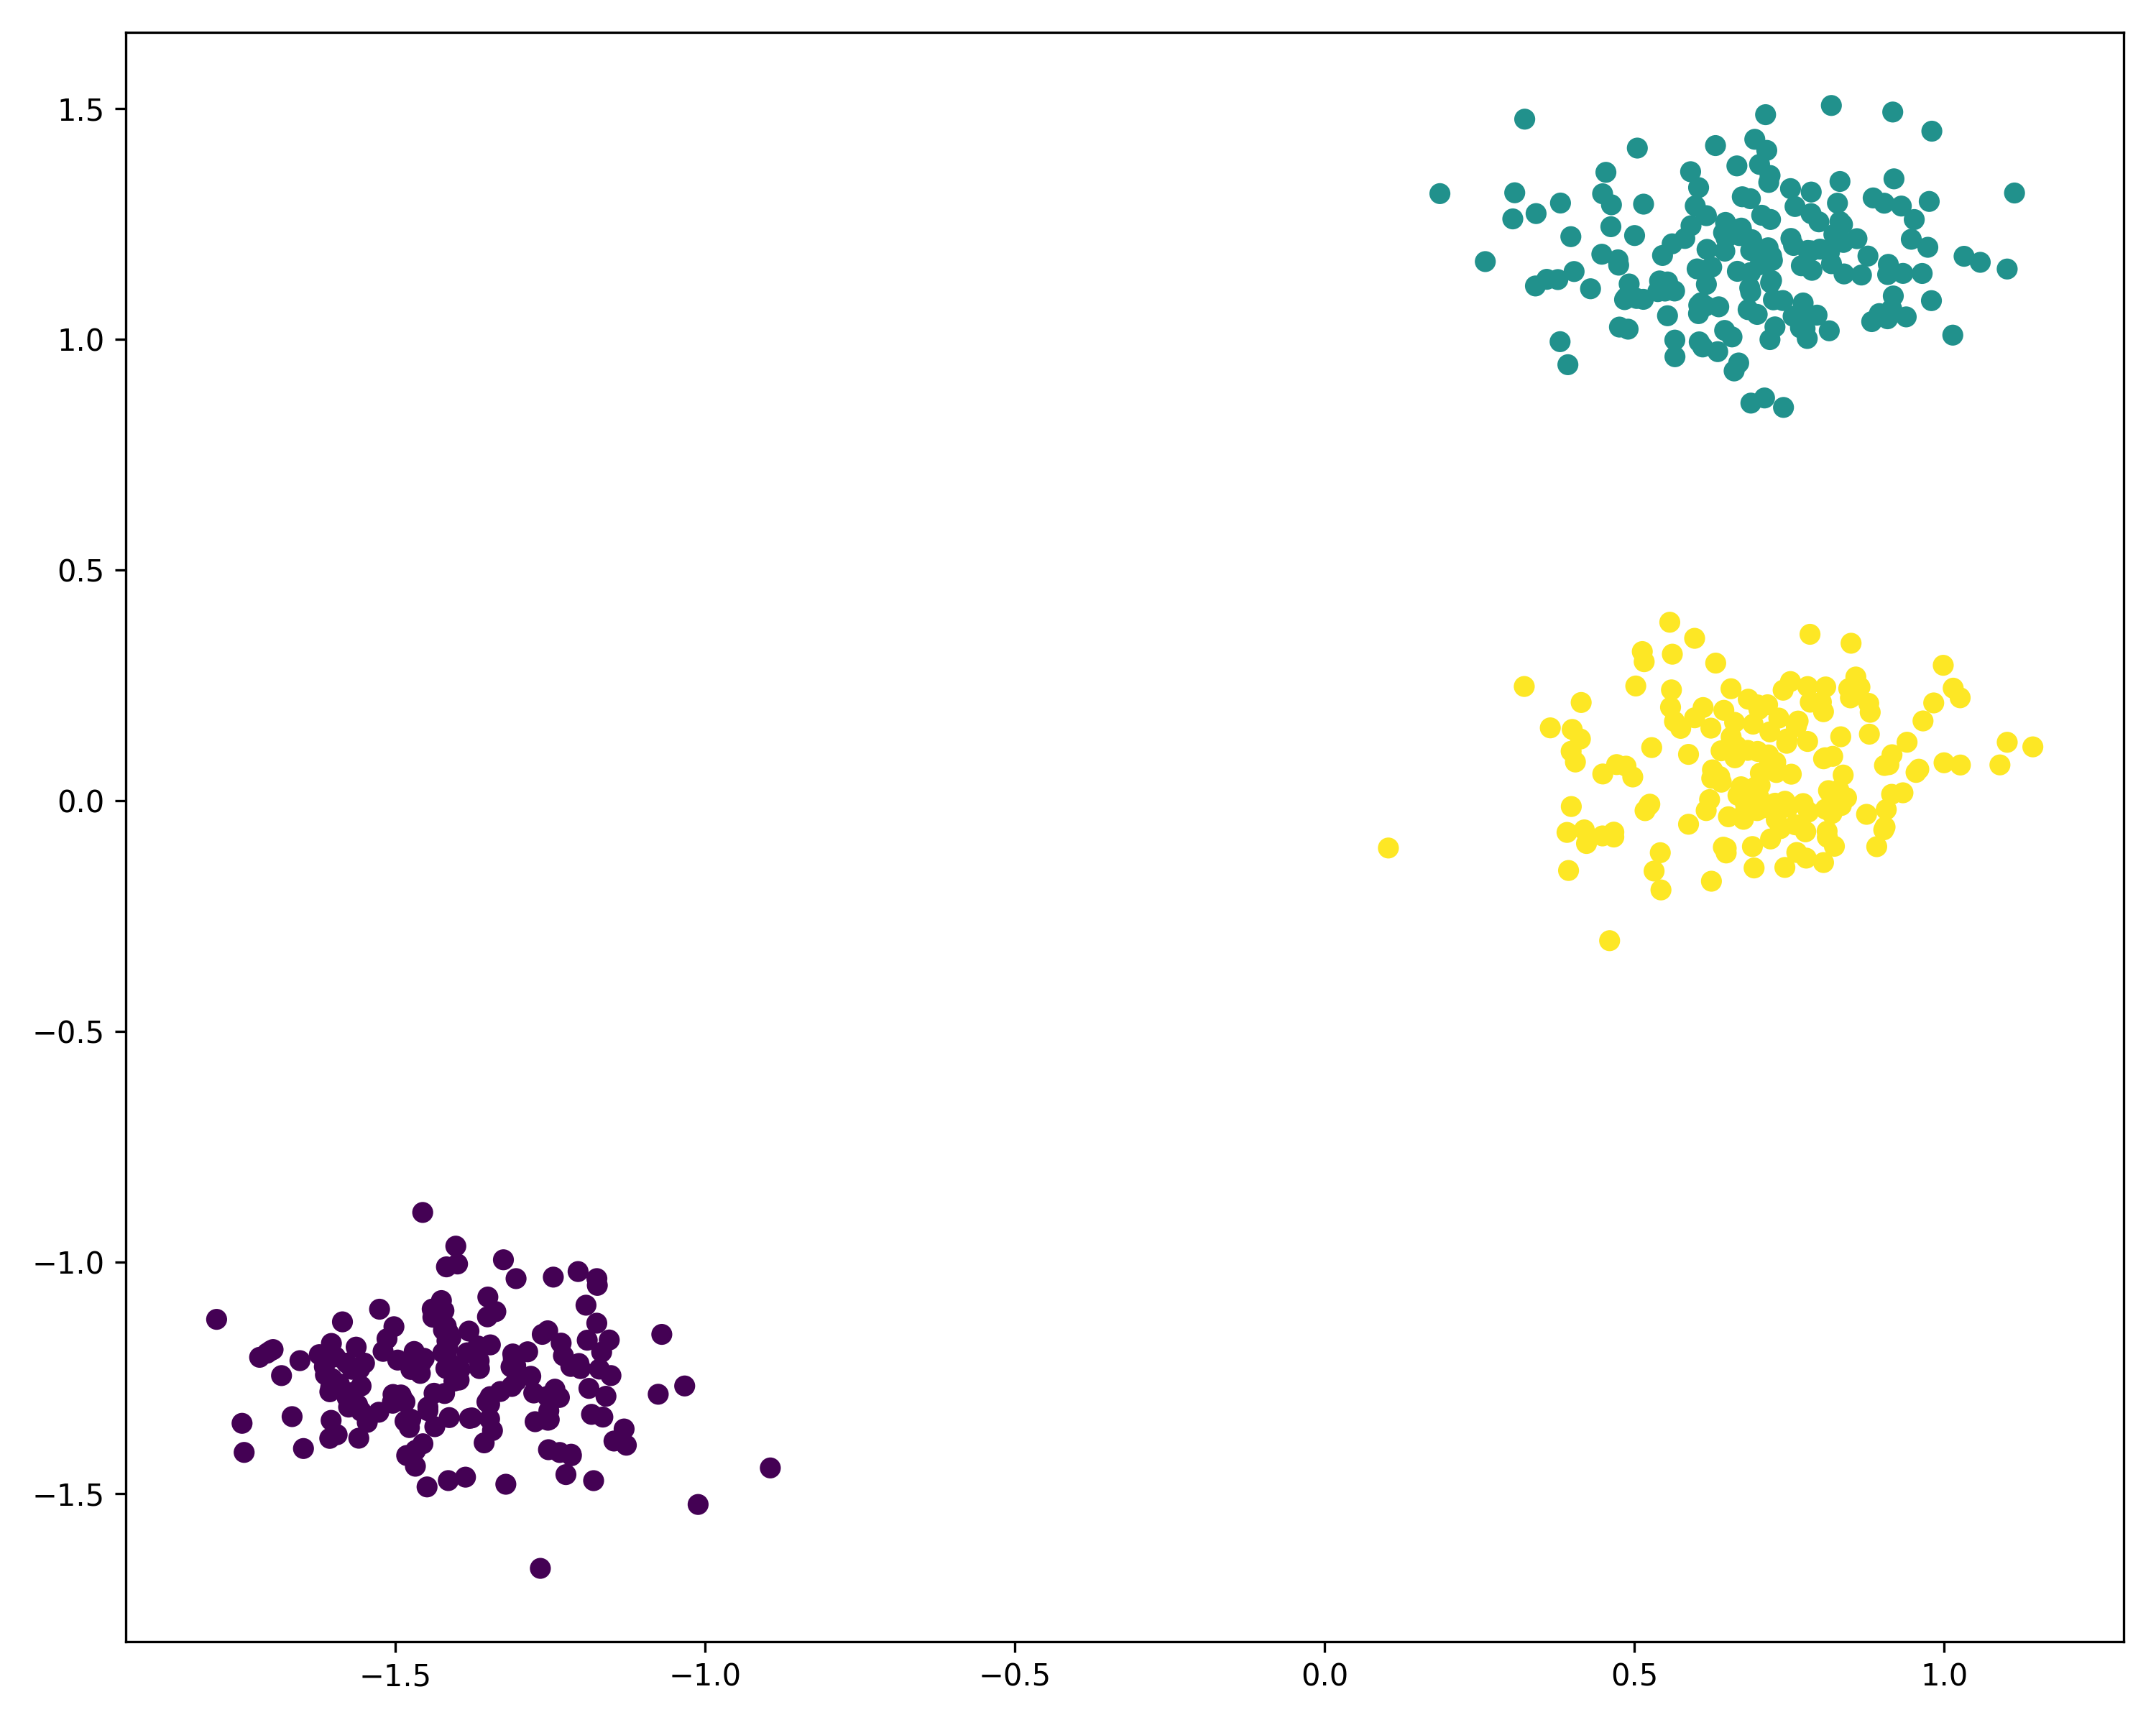
\includegraphics[width=\linewidth]{images/claire/random_n0_blobs_dbscan_eps_0_4_min_samples_2.png}
\end{minipage}

\vspace{0.02cm}
\begin{minipage}{.35\textwidth}
  \centering
  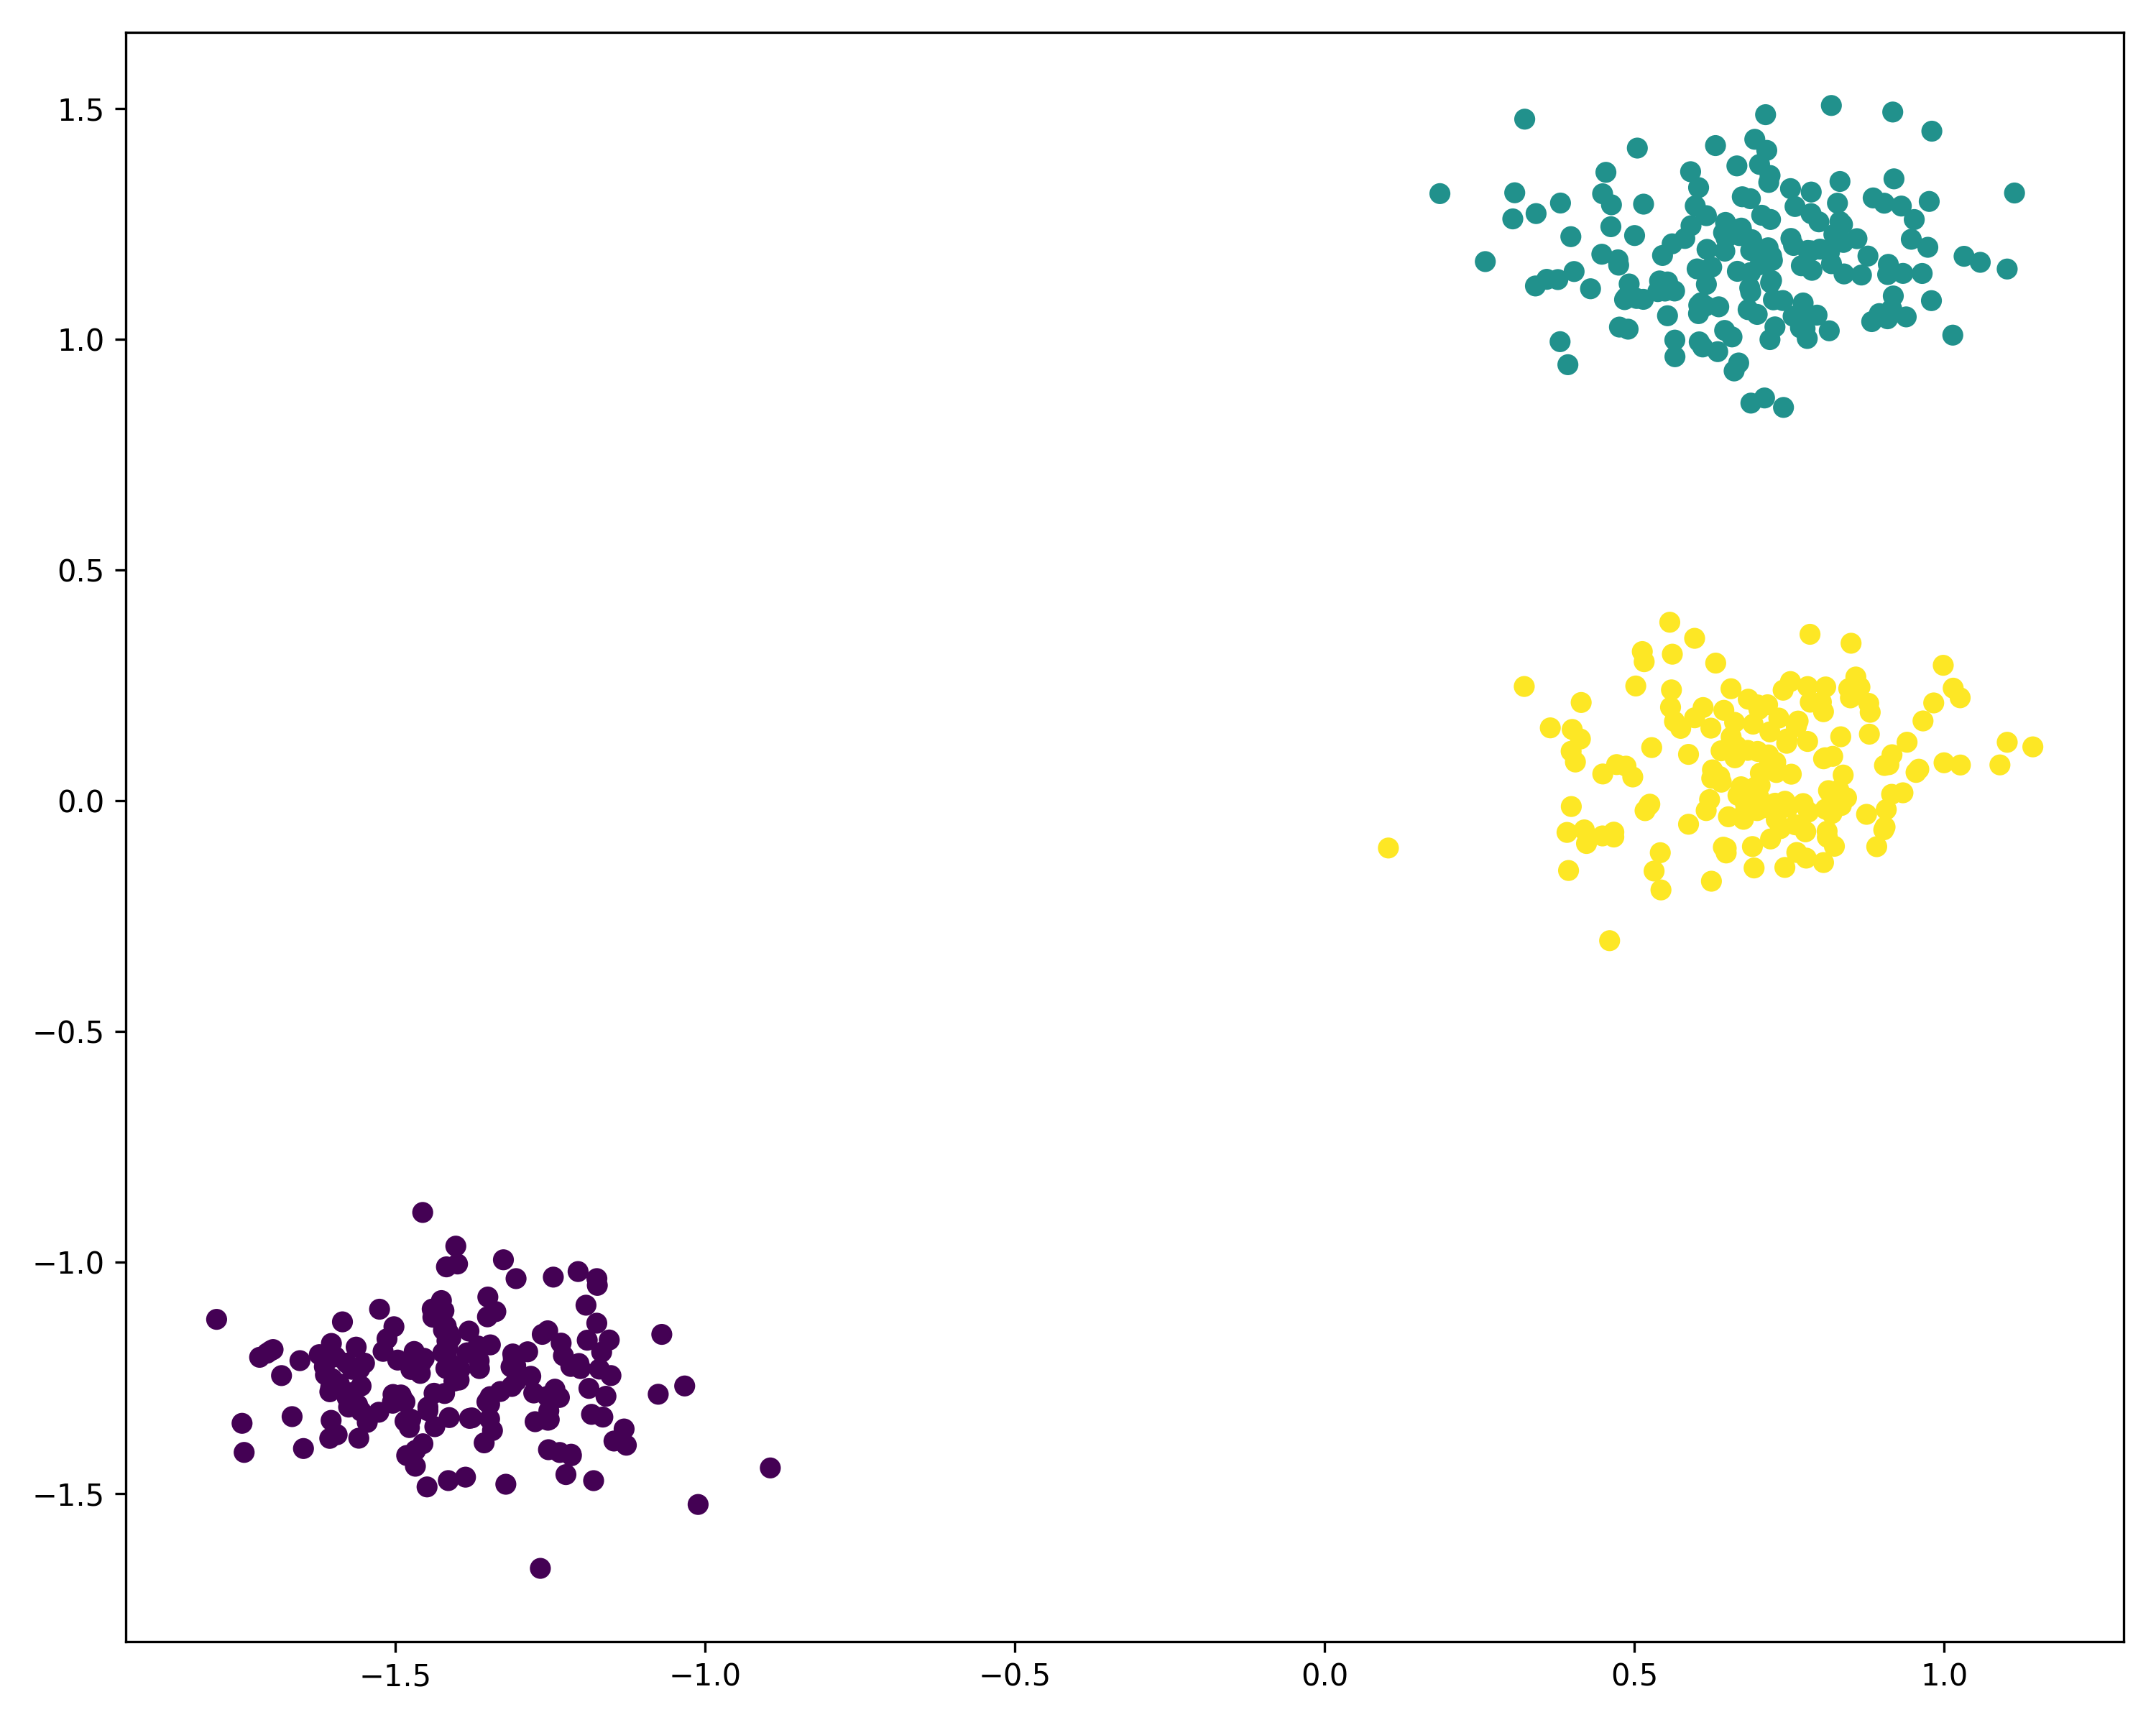
\includegraphics[width=\linewidth]{images/claire/random_n0_blobs_kernel_kmeans_n_clusters_3_kernel_gak_random_state_0.png}

\end{minipage}%
\hspace{0.02cm}
\begin{minipage}{.35\textwidth}
  \centering
  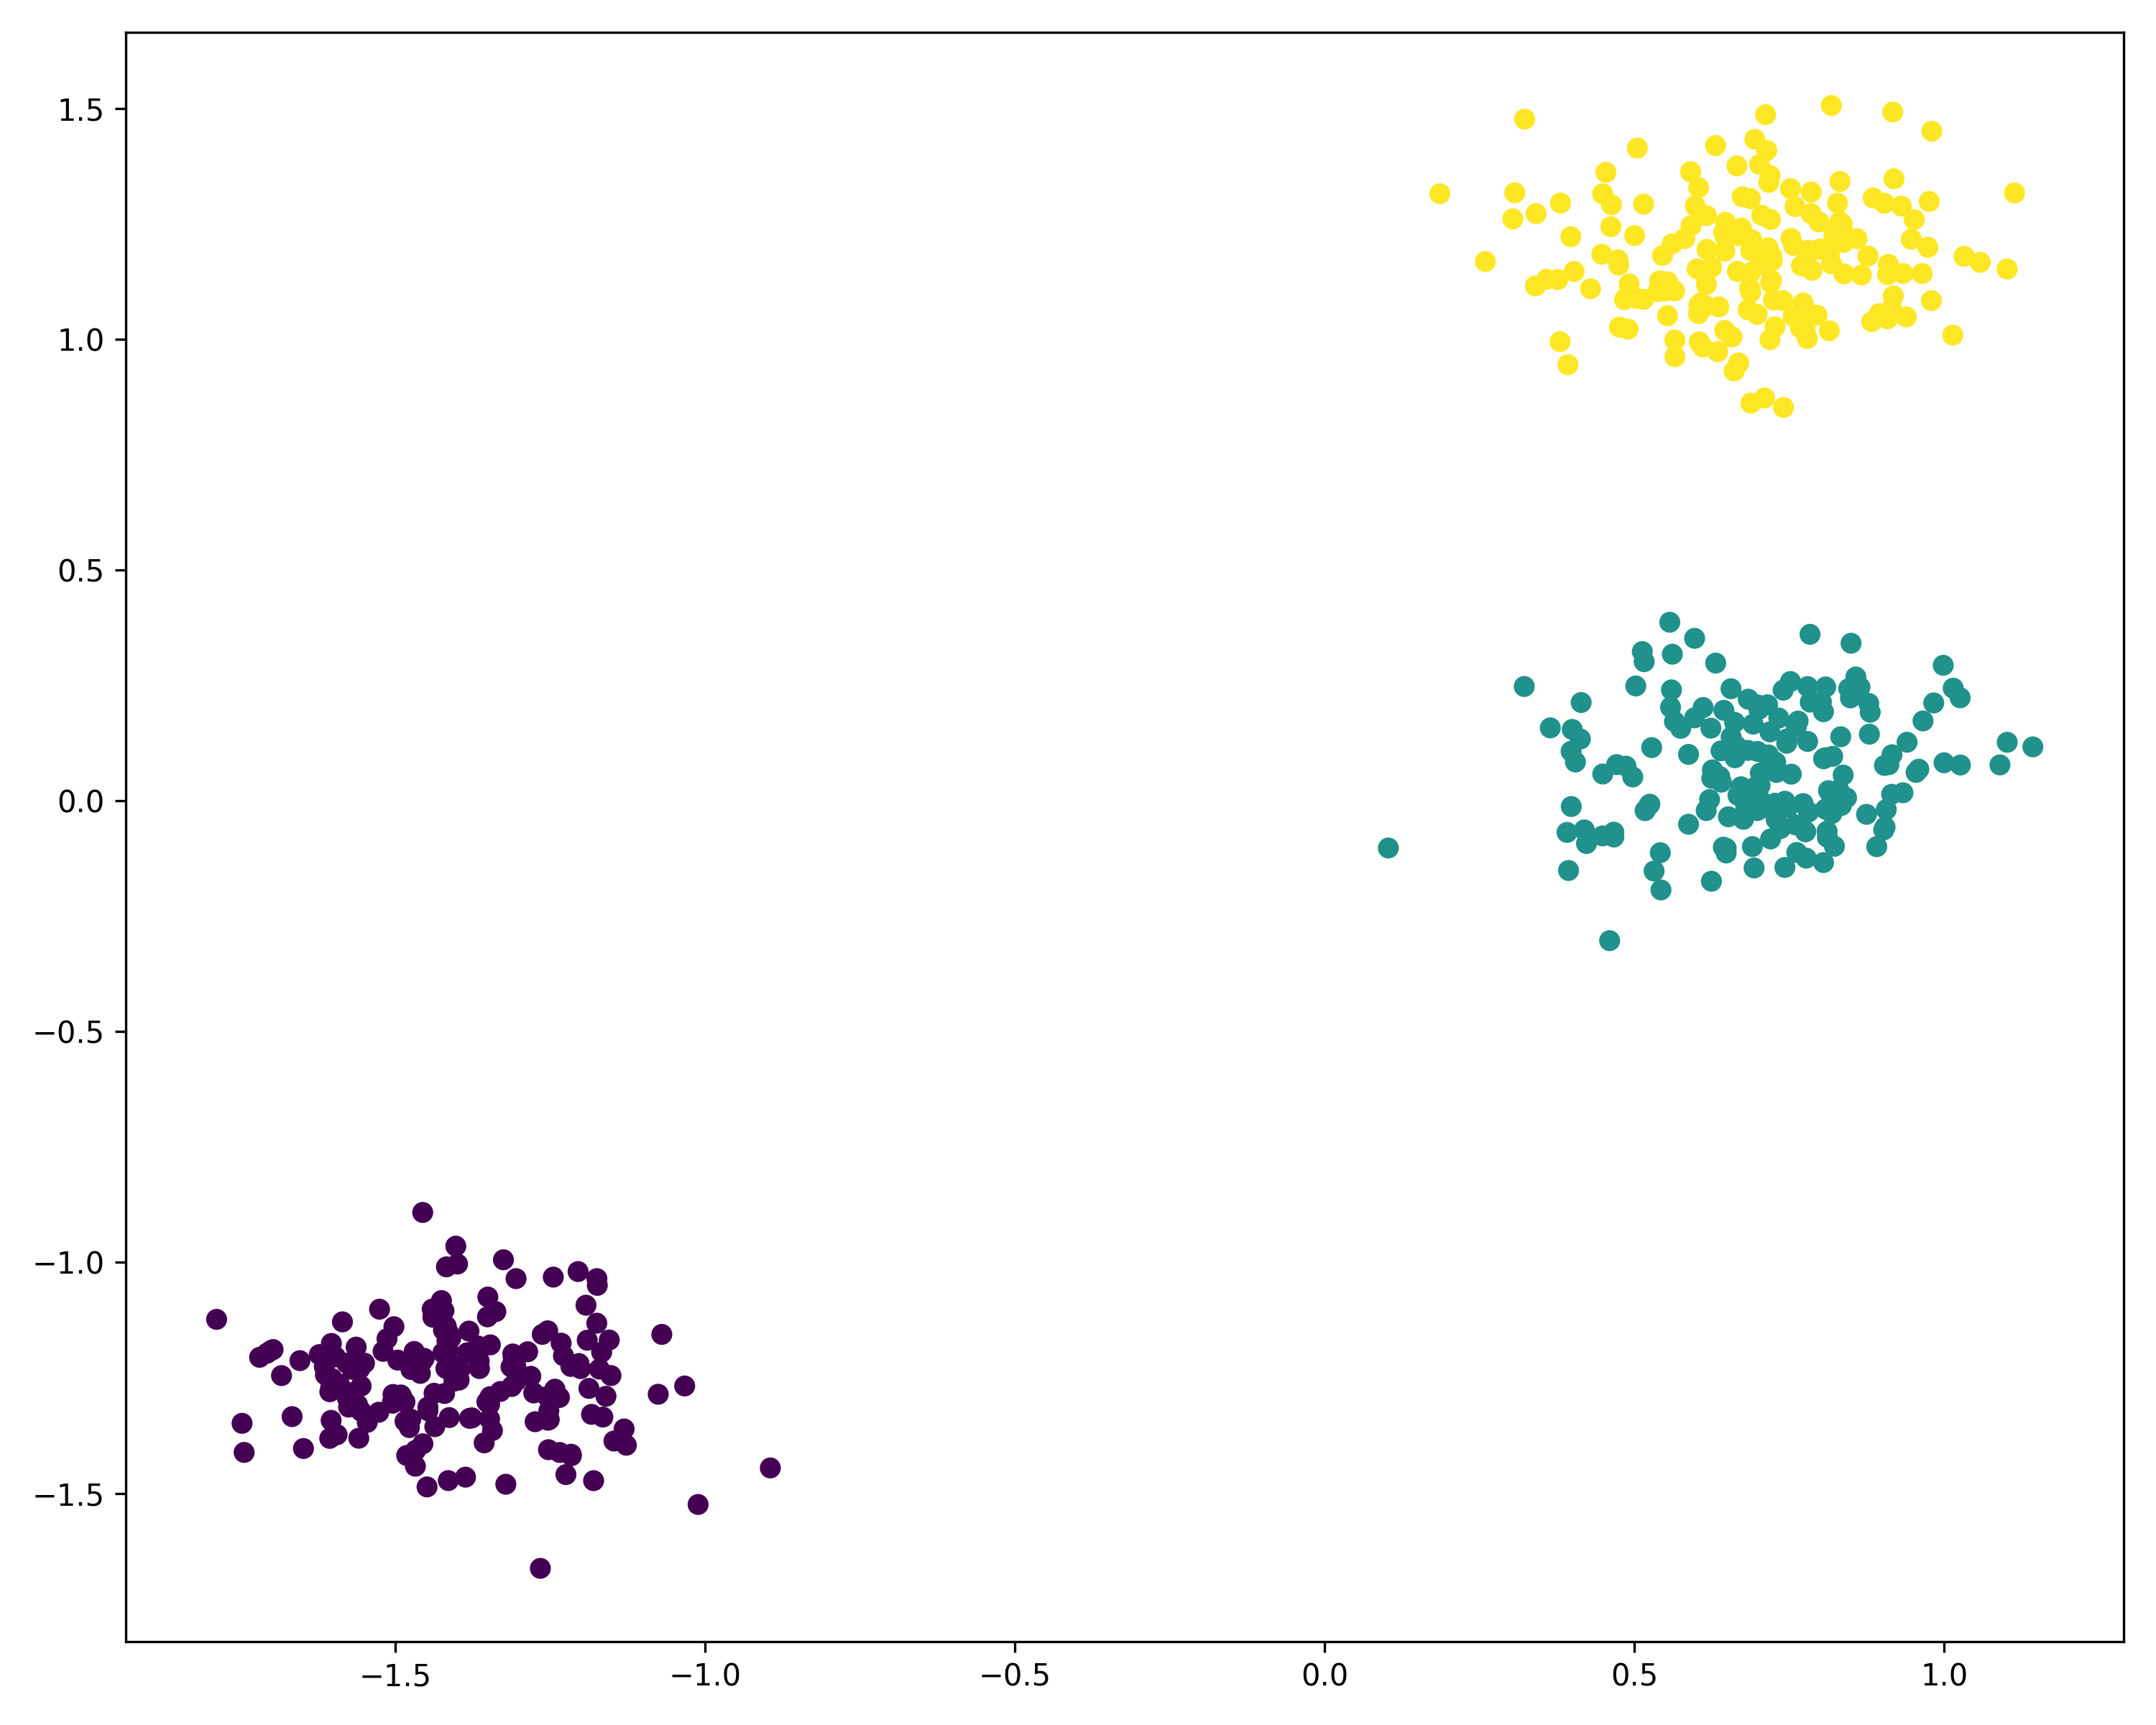
\includegraphics[width=\linewidth]{images/claire/random_n0_blobs_spectral_clustering_n_clusters_3_eigen_solver_arpack_affinity_nearest_neighbors.png}
\end{minipage}
\caption{A melhor partição foi encontrada por Mean Shift, Spectral Clustering ($K = 3$), Kernel K-means ($K = 3$), DBSCAN ($\epsilon = \{0.3, 0.4\}$) e OPTICS (\textsf{xi} $= 0.1$ e \textsf{min\_cluster\_size} $= 0.2$), para o conjunto de dados Blobs.}

\end{figure}


\begin{figure}
\centering
\begin{minipage}{.5\textwidth}
  \centering
  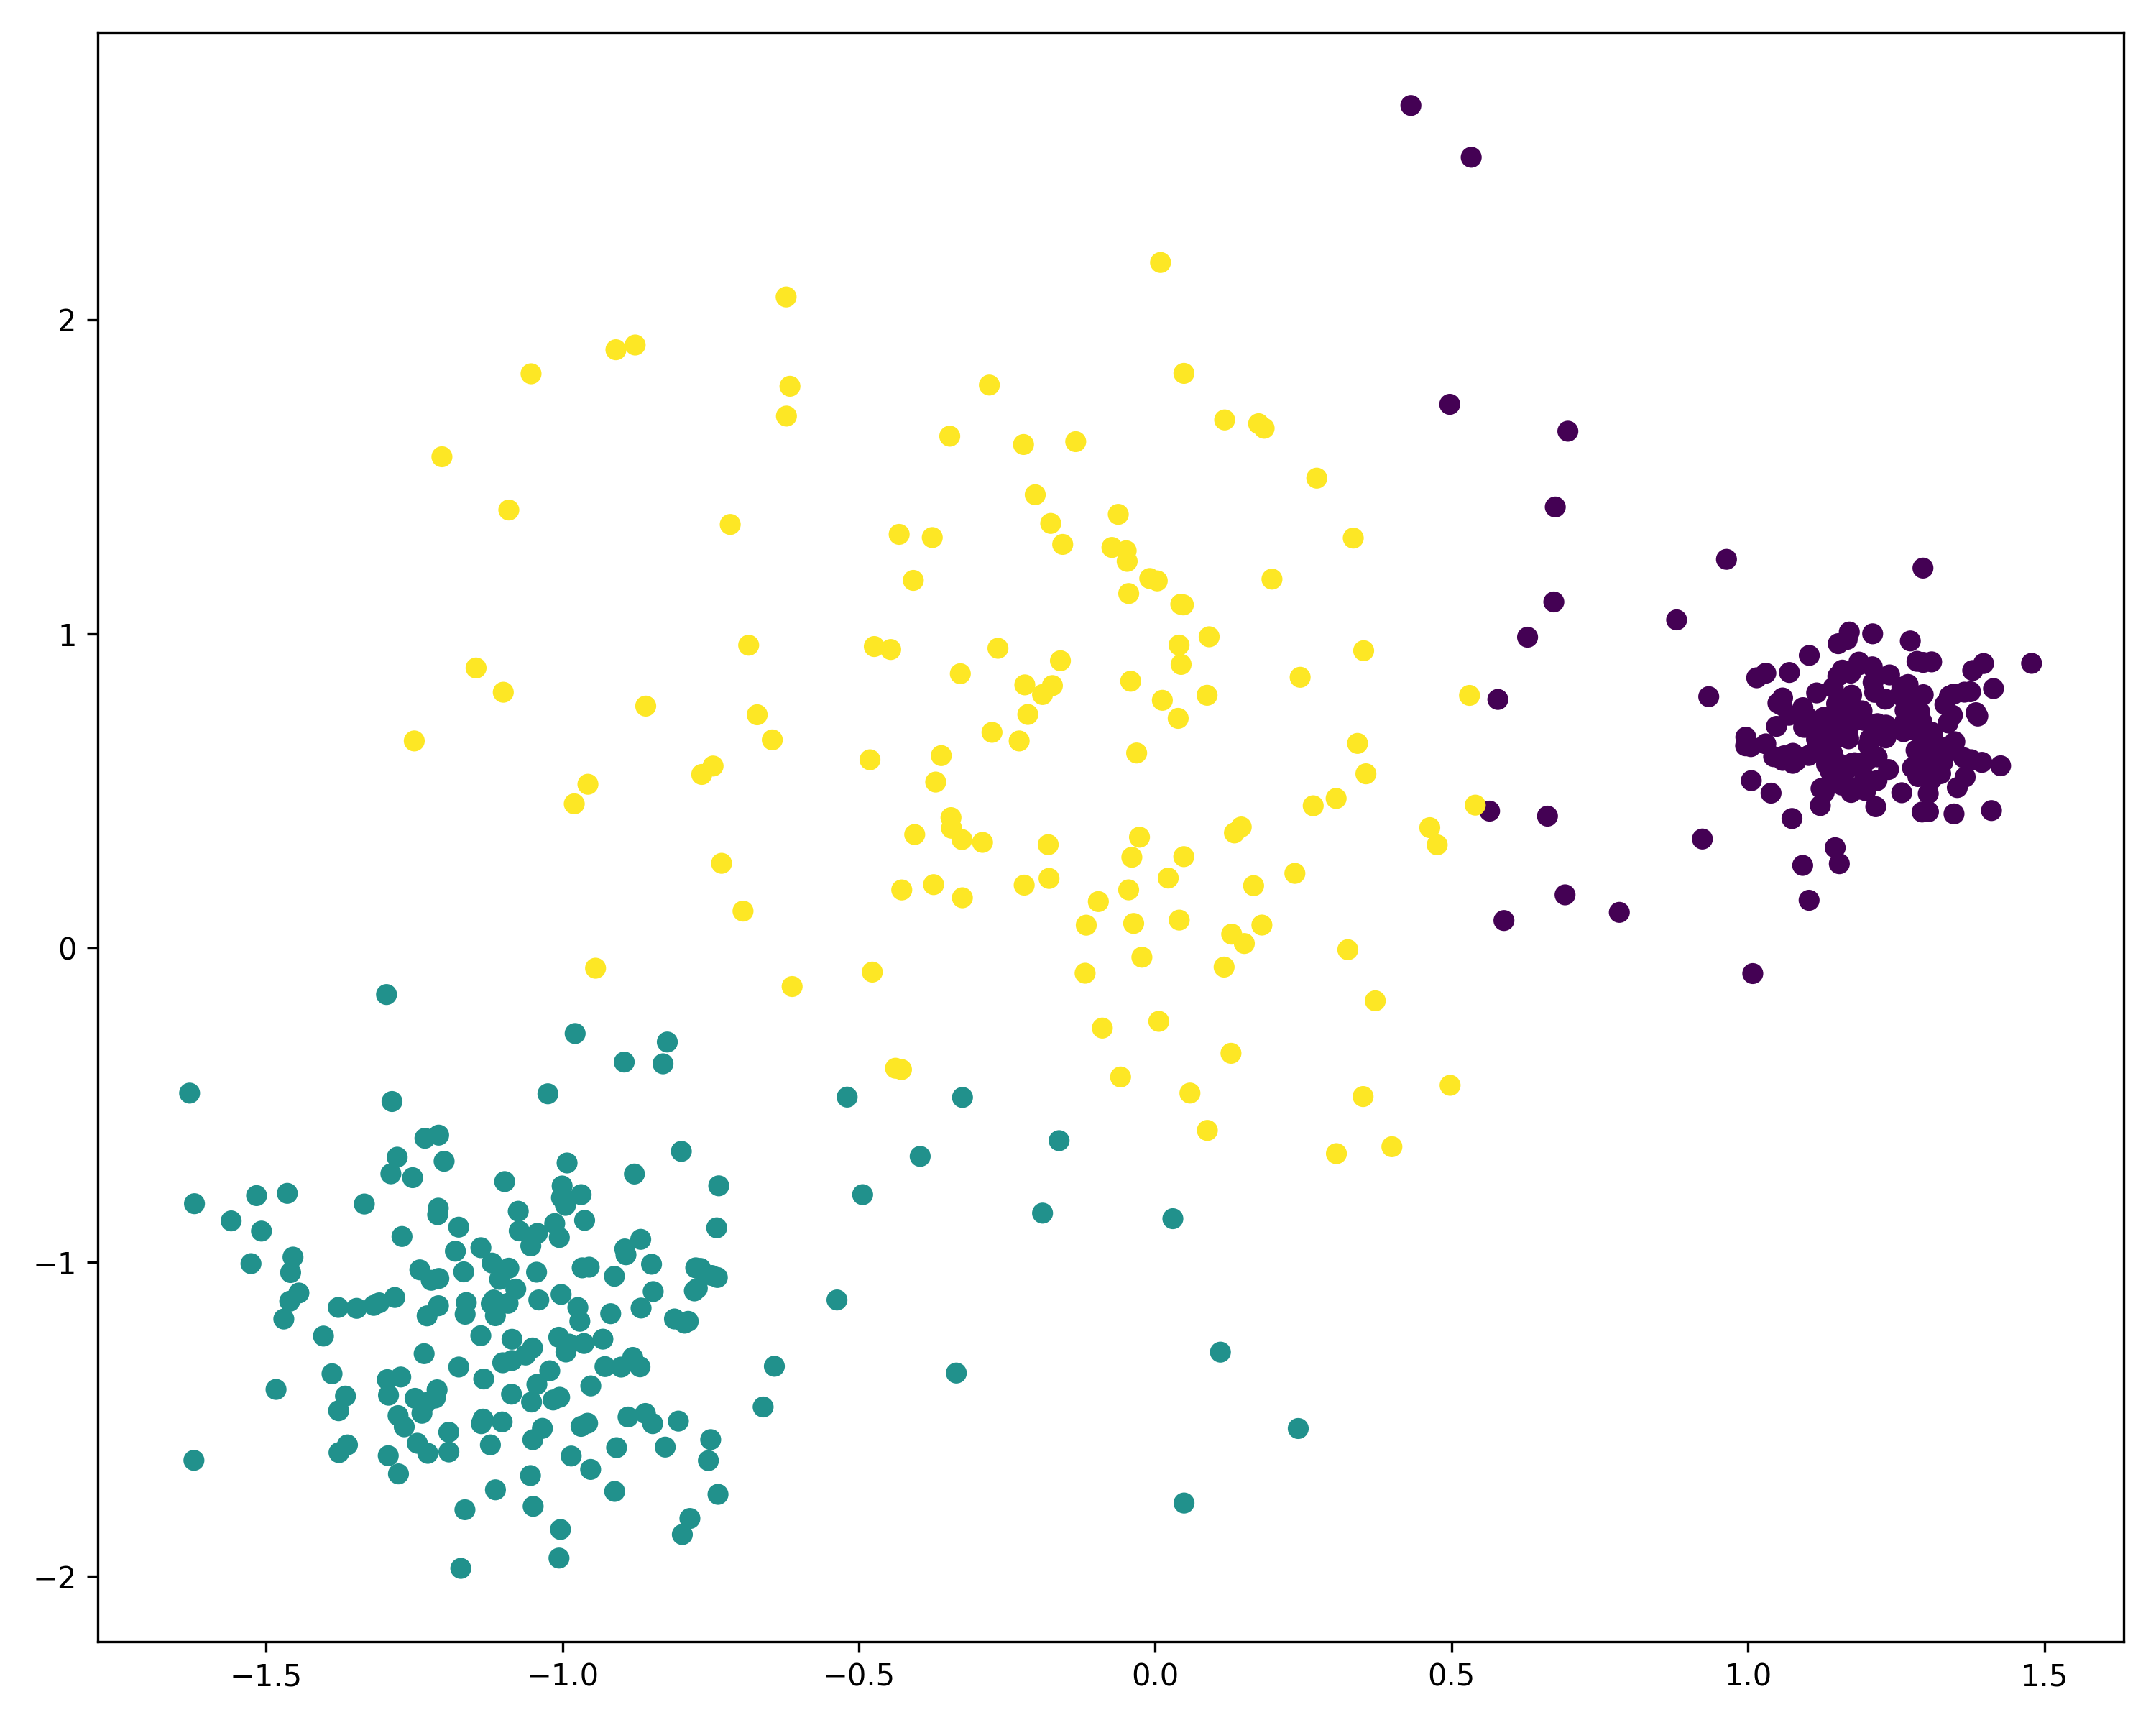
\includegraphics[width=\linewidth]{images/claire/random_n0_varied_mean_shift_.png}
\end{minipage}%
\caption{A melhor partição encontrada por Mean Shift, para o conjunto de dados Varied.}

\end{figure}

%% noisy_circles
\begin{figure}
\centering
\begin{minipage}{.4\textwidth}
  \centering
  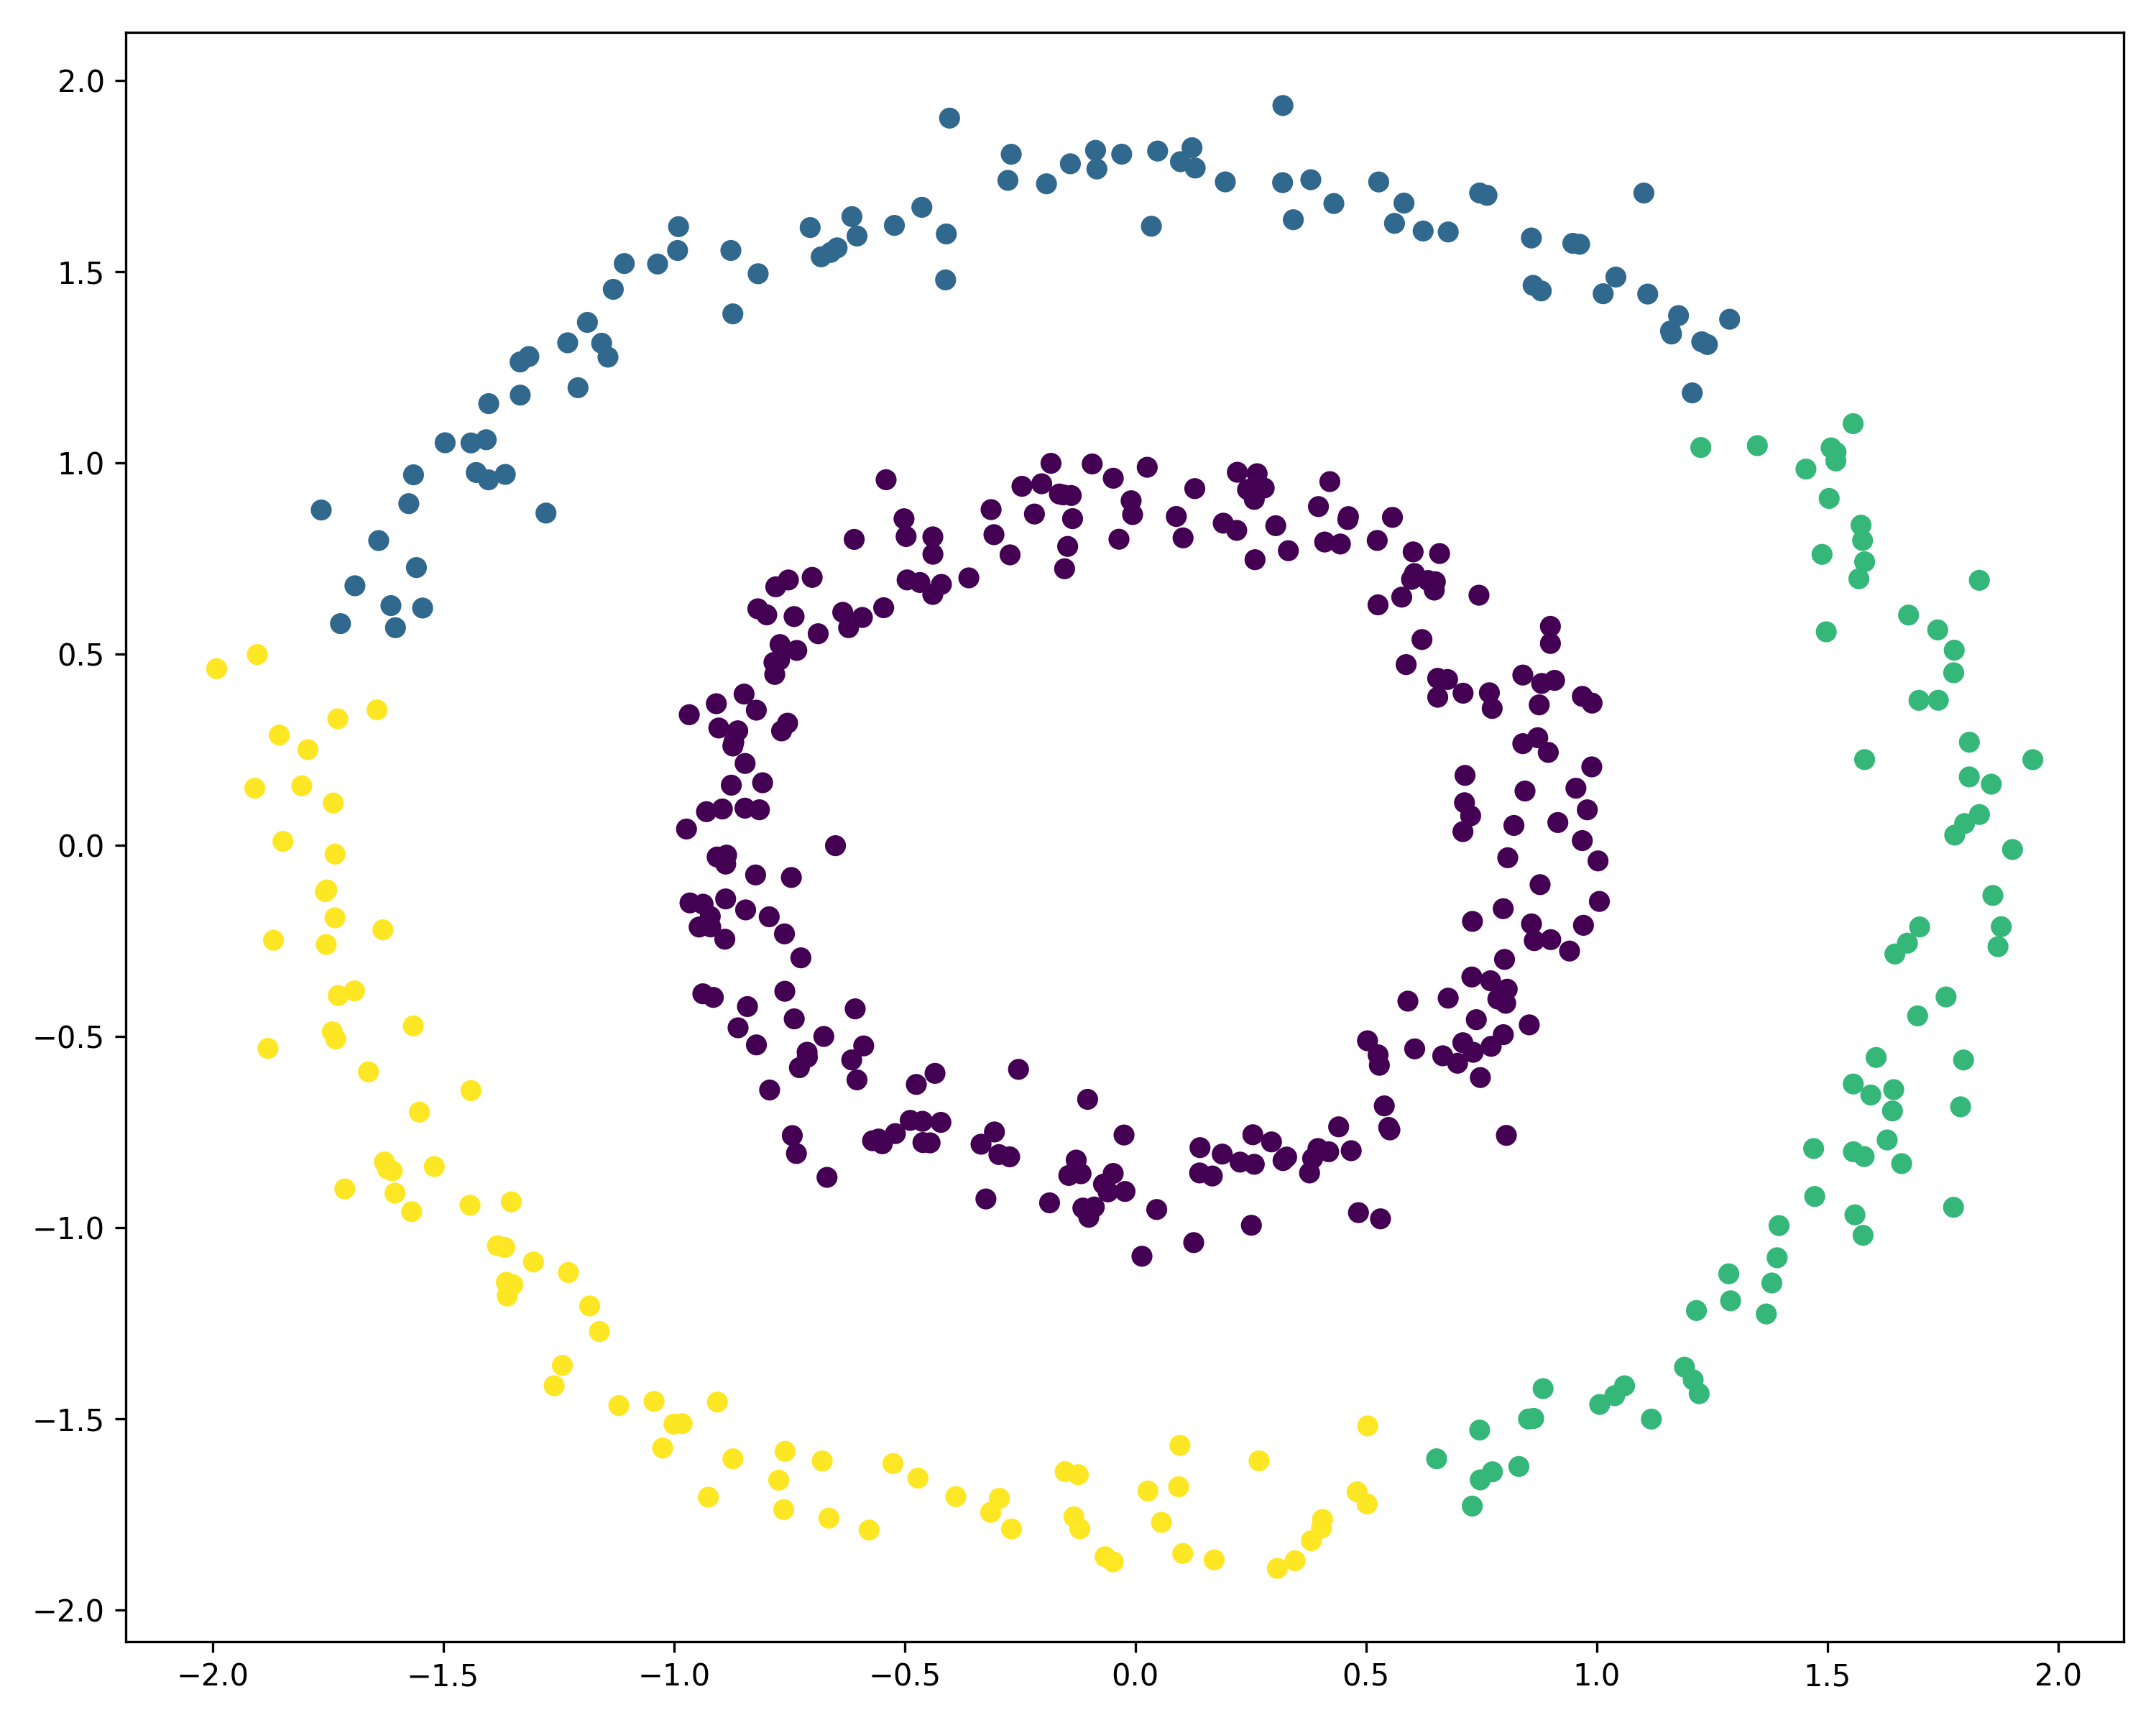
\includegraphics[width=\linewidth]{images/claire/random_n0_noisy_circles_spectral_clustering_n_clusters_4_eigen_solver_arpack_affinity_nearest_neighbors.png}
\end{minipage}%
\hspace{0.02cm}
\begin{minipage}{.4\textwidth}
  \centering
  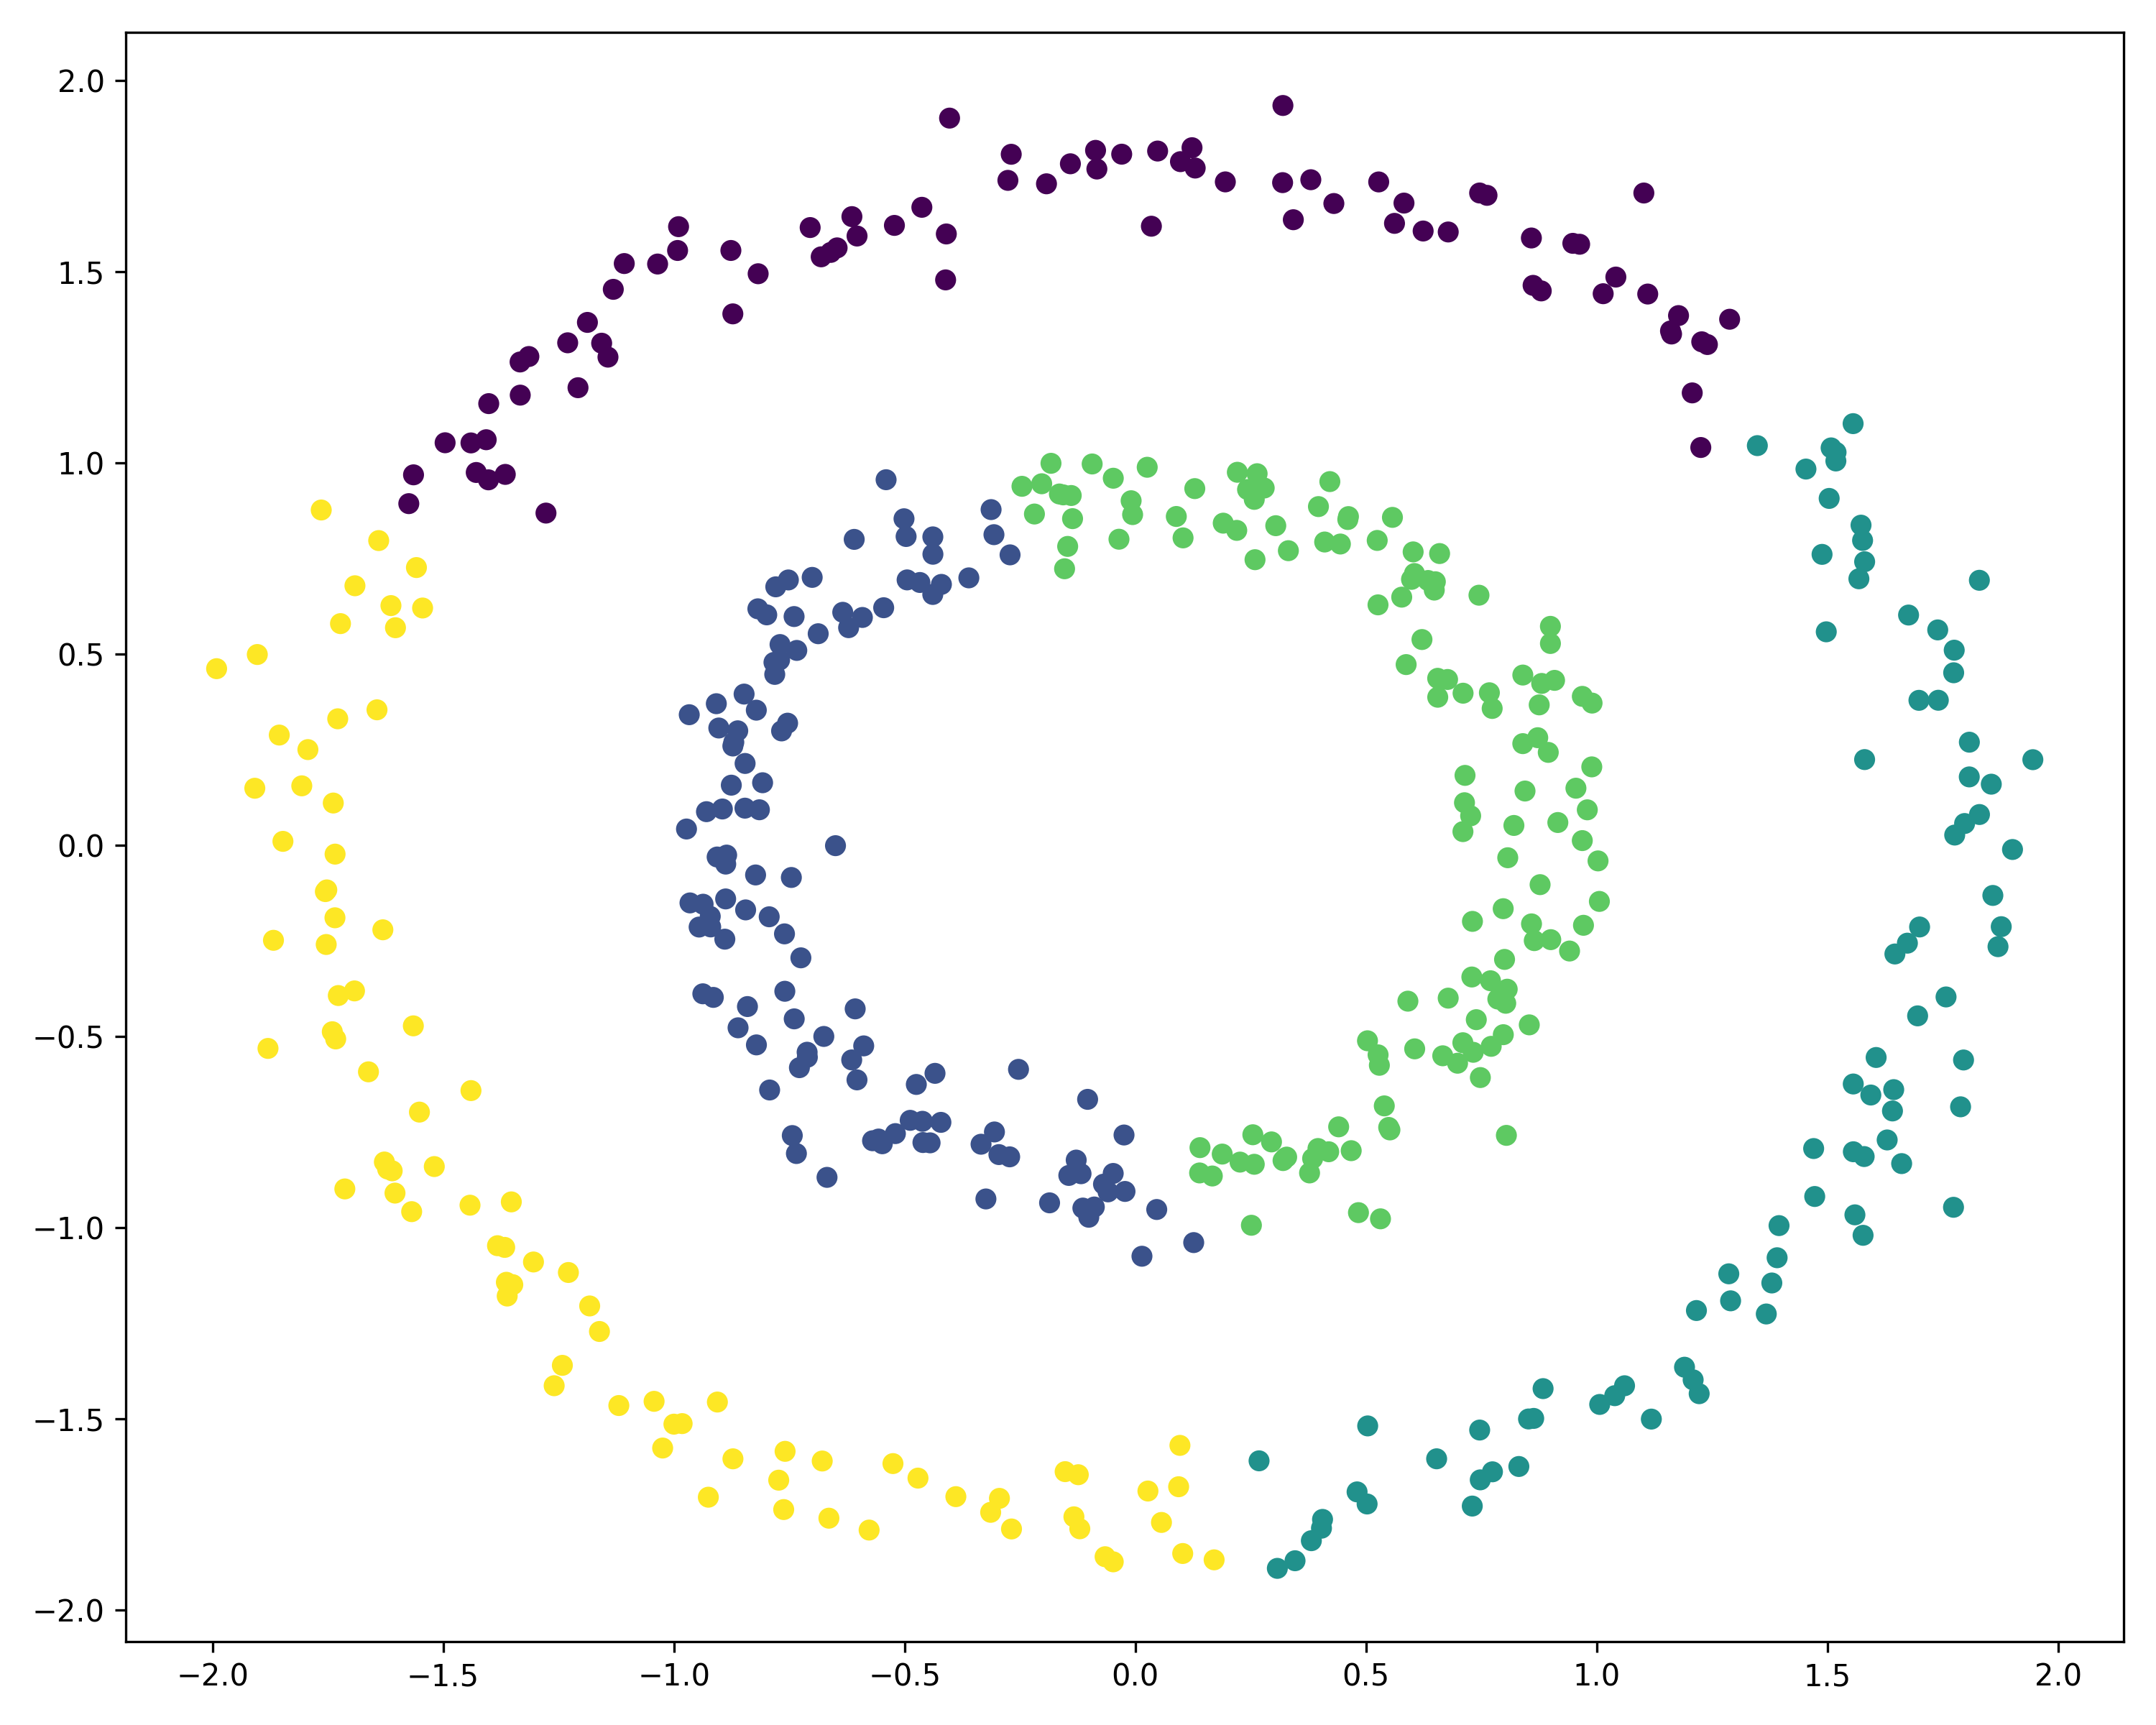
\includegraphics[width=\linewidth]{images/claire/random_n0_noisy_circles_spectral_clustering_n_clusters_5_eigen_solver_arpack_affinity_nearest_neighbors.png}
\end{minipage}
\caption{Melhor partição encontrada por Spectral Clustering ($K = \{4, 5\}$), para o conjunto de dados Noisy Circles.}
\end{figure}

%%% no_structure
\begin{figure}
\centering
\begin{minipage}{.8\textwidth}
  \centering
  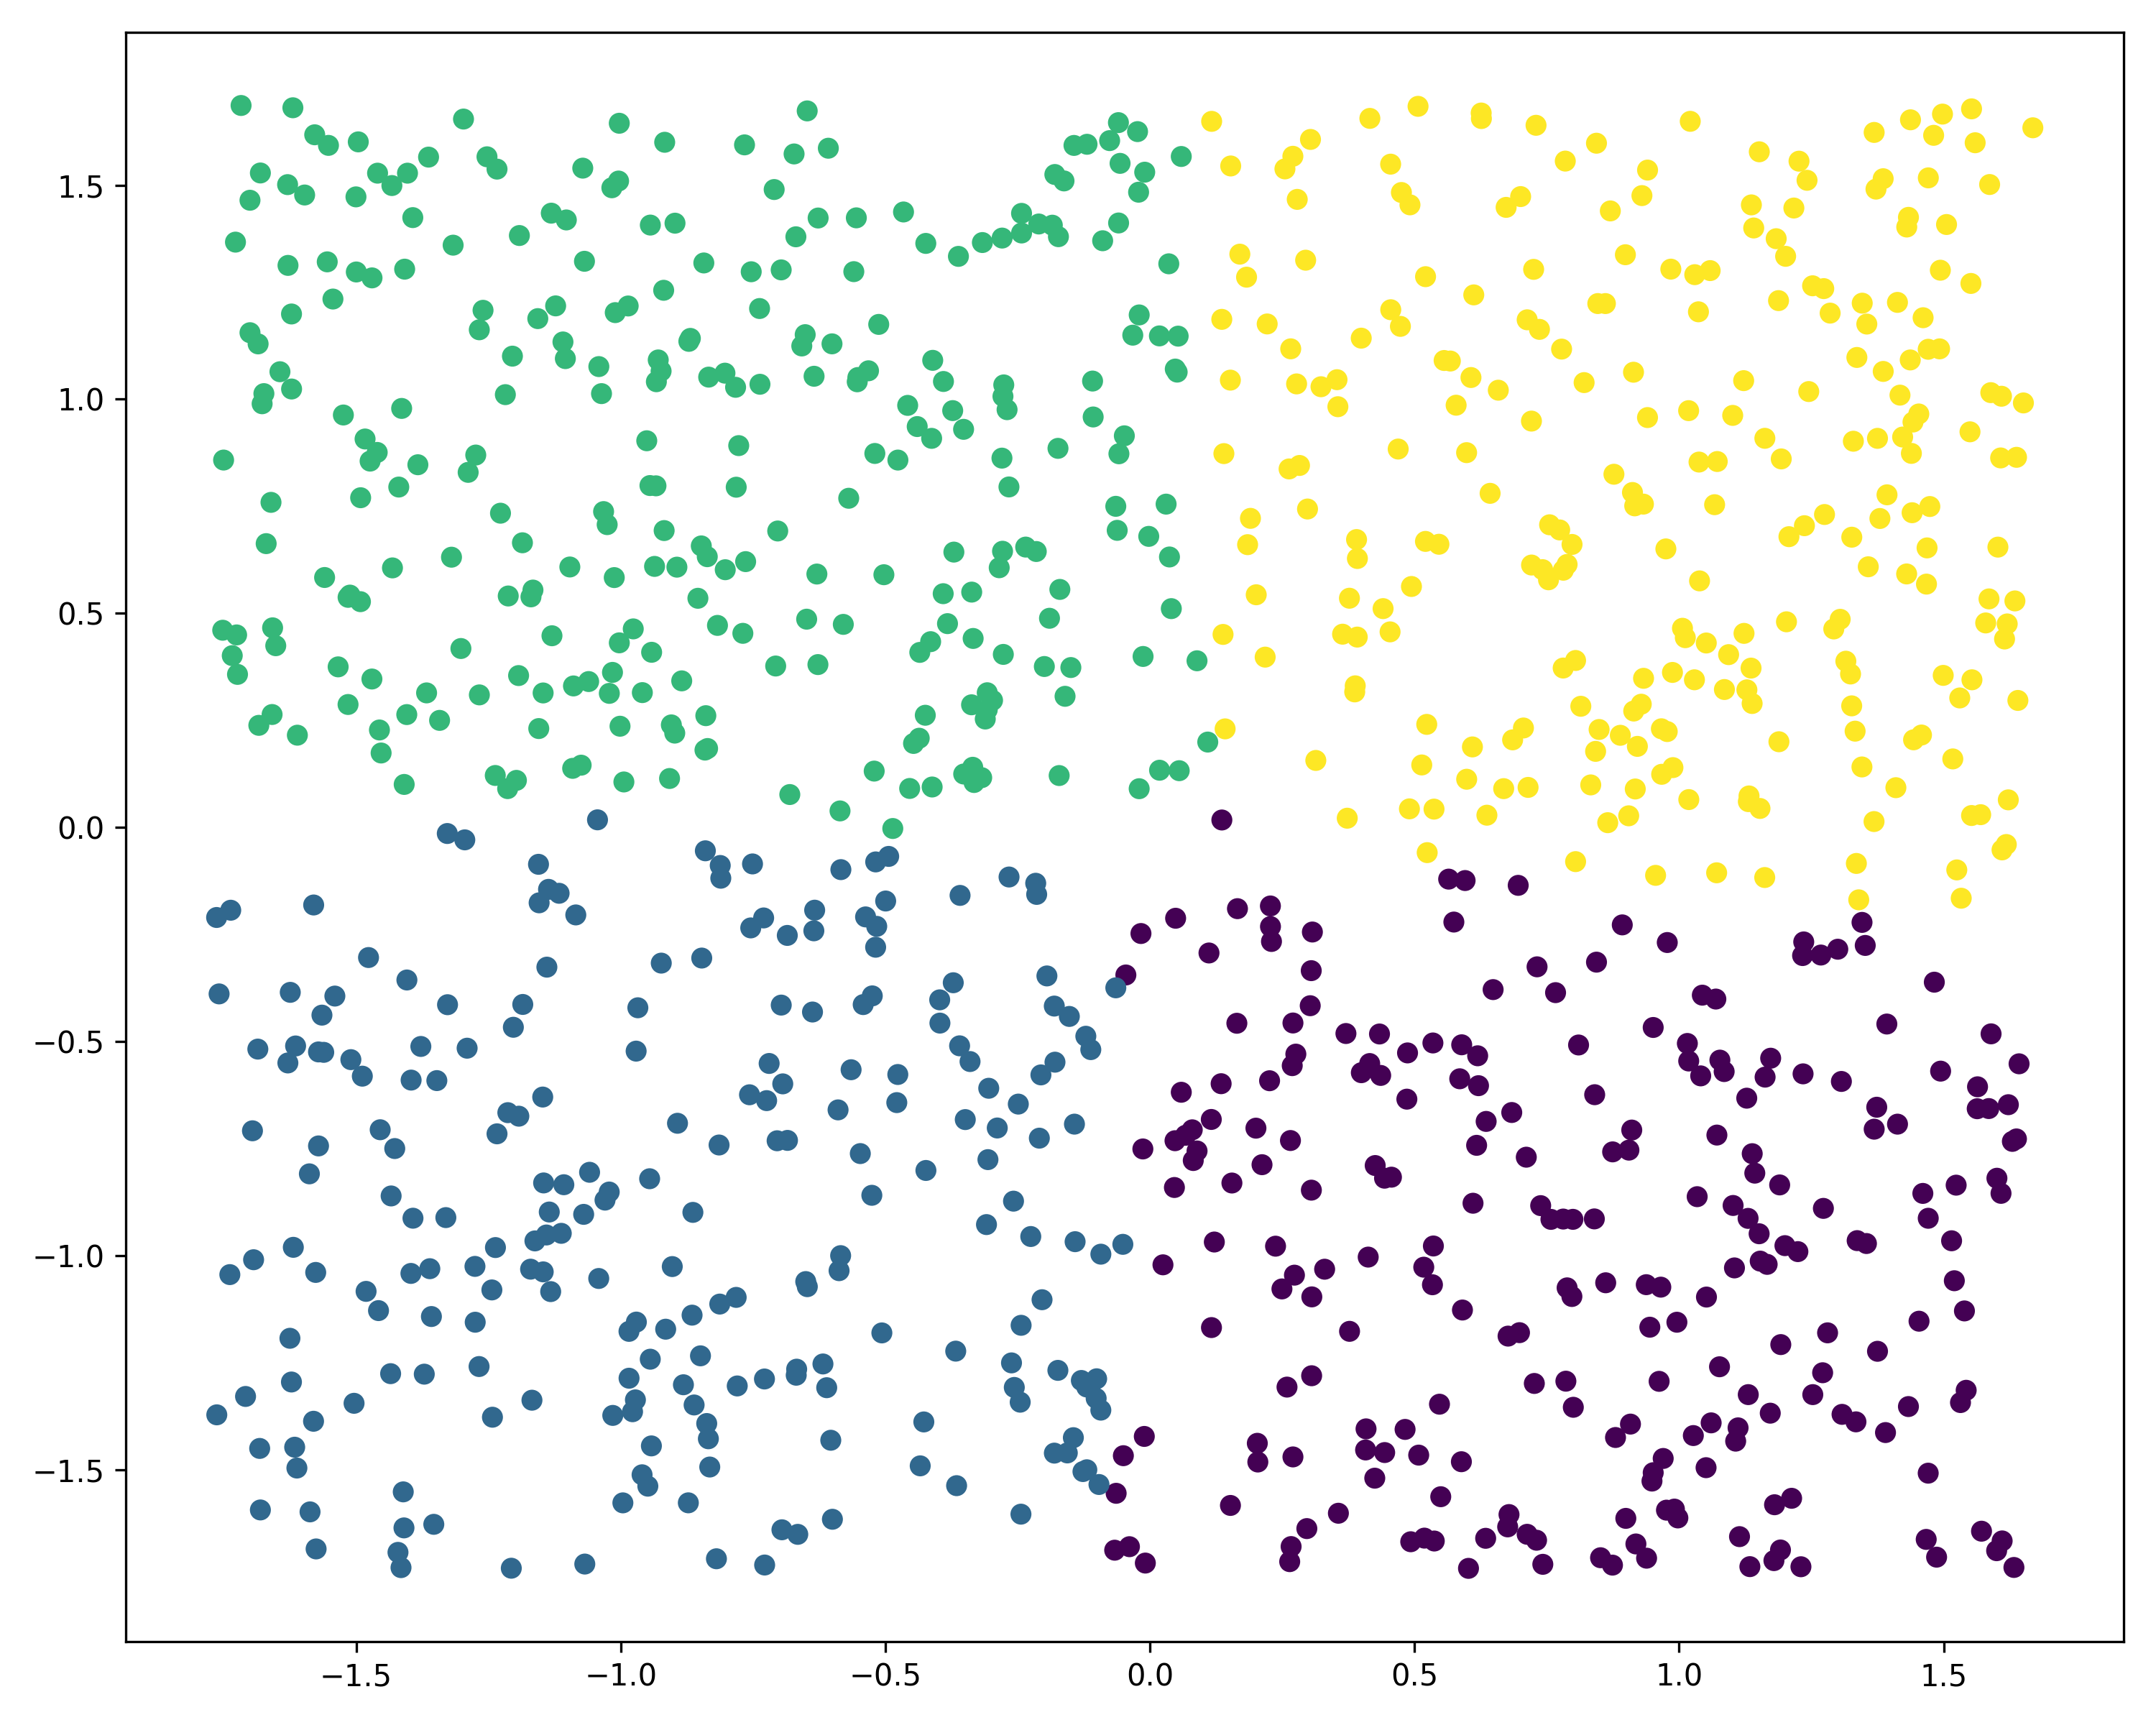
\includegraphics[width=\linewidth]{images/claire/random_n0_no_structure_kernel_kmeans_n_clusters_4_kernel_gak_random_state_0.png}
\end{minipage}%
\caption{Melhor partição encontrada por Kernel K-means ($K = 4$), para o conjunto de dados No Structure.}

\end{figure}

\begin{figure}
\centering
\begin{minipage}{.4\textwidth}
  \centering
  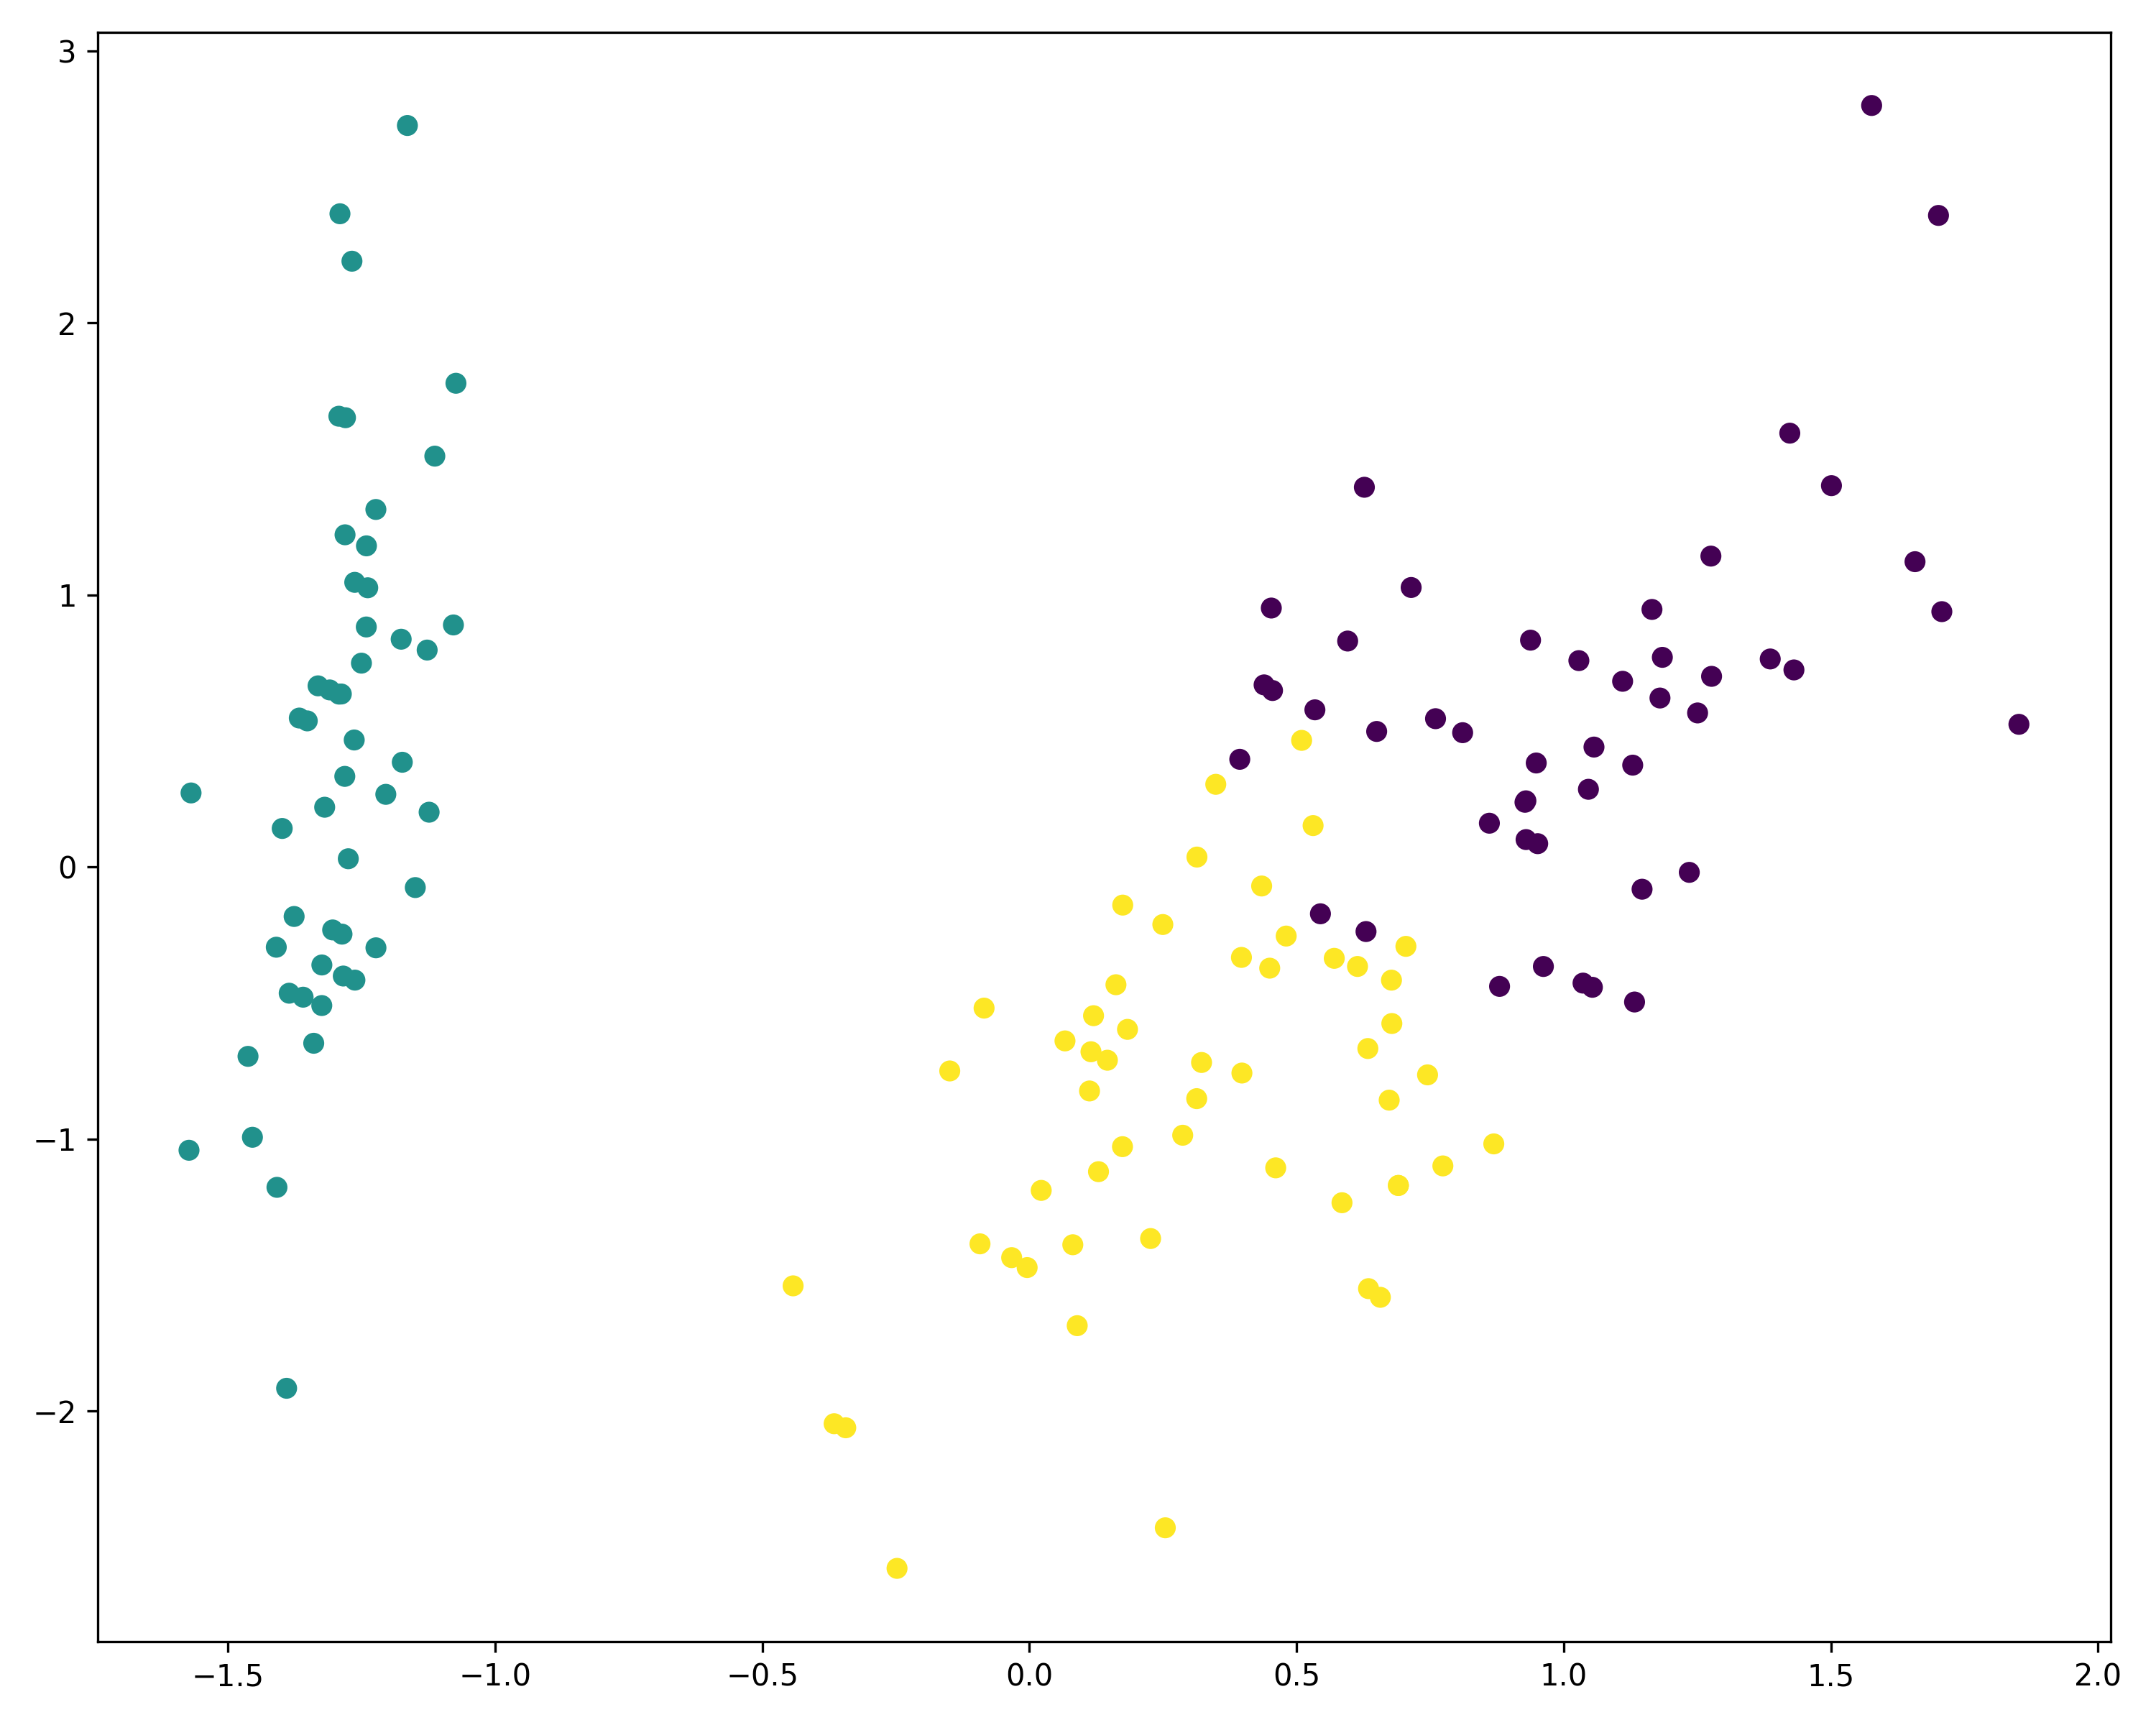
\includegraphics[width=\linewidth]{images/claire/random_n0_iris_kmeans_n_clusters_3.png}
\end{minipage}%
\hspace{0.02cm}
\begin{minipage}{.4\textwidth}
  \centering
  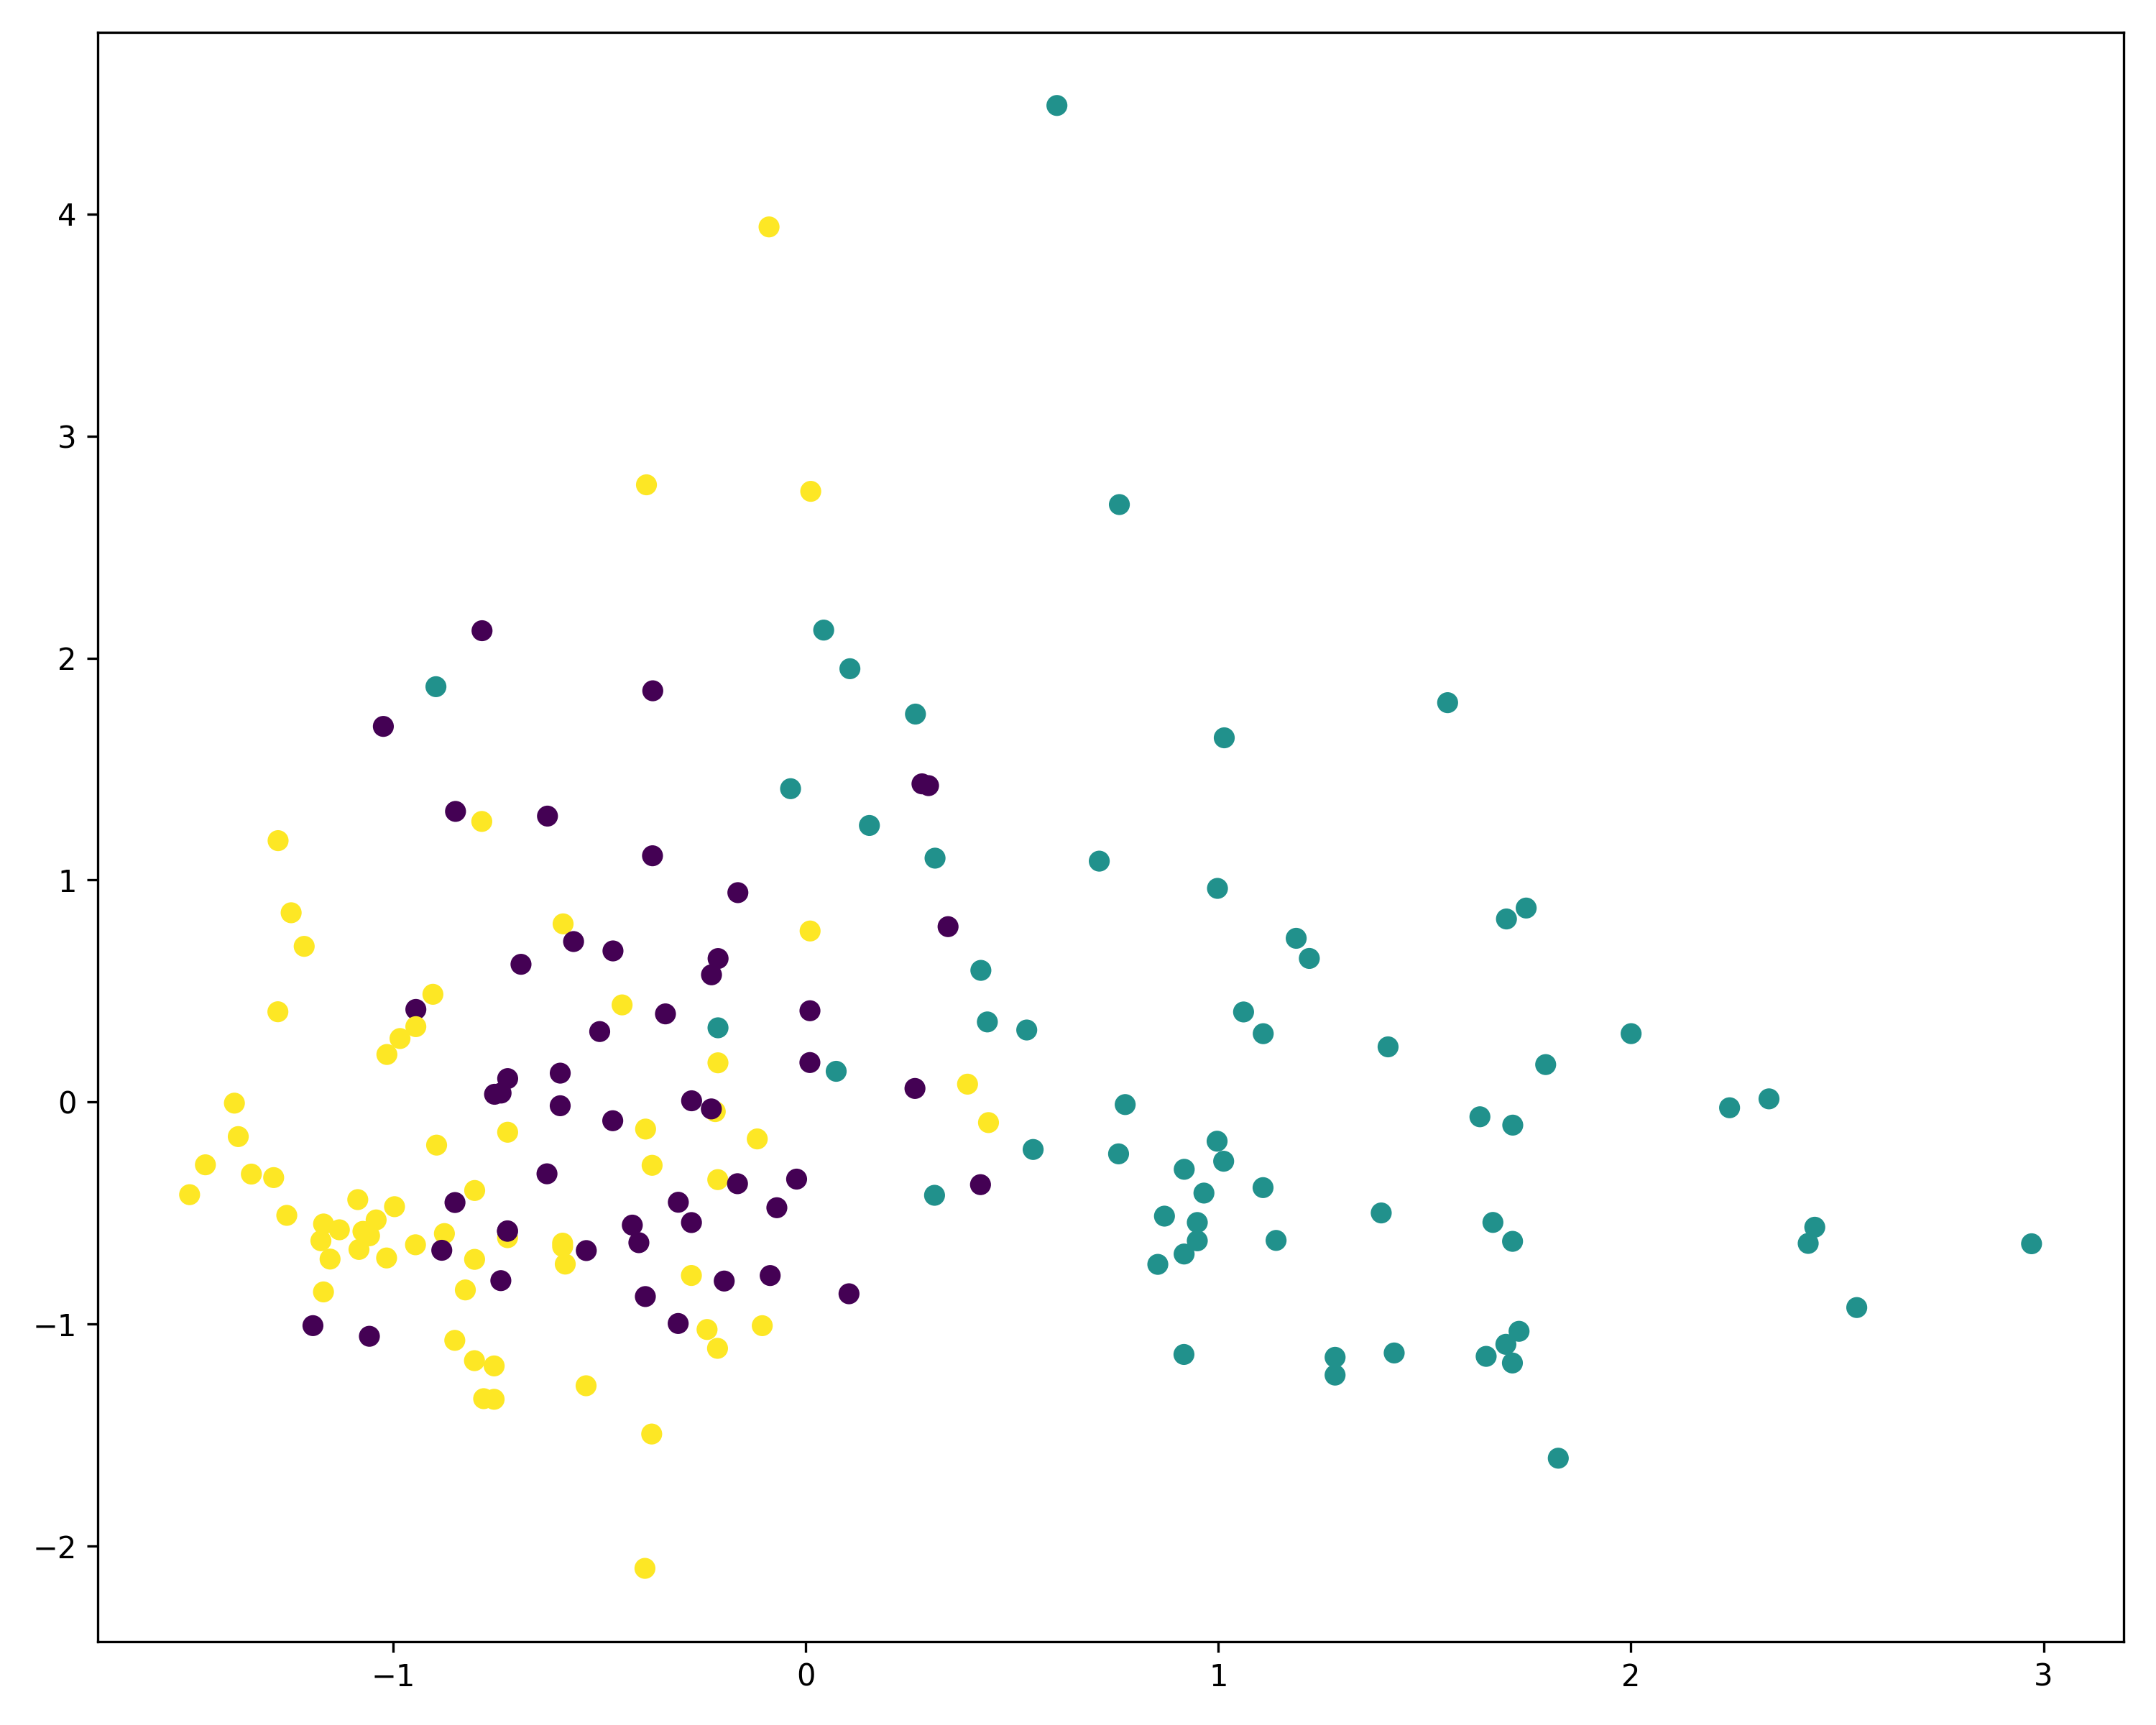
\includegraphics[width=\linewidth]{images/claire/random_n0_wine_kmeans_n_clusters_3.png}
\end{minipage}
\vspace{0.02cm}
\begin{minipage}{.4\textwidth}
  \centering
  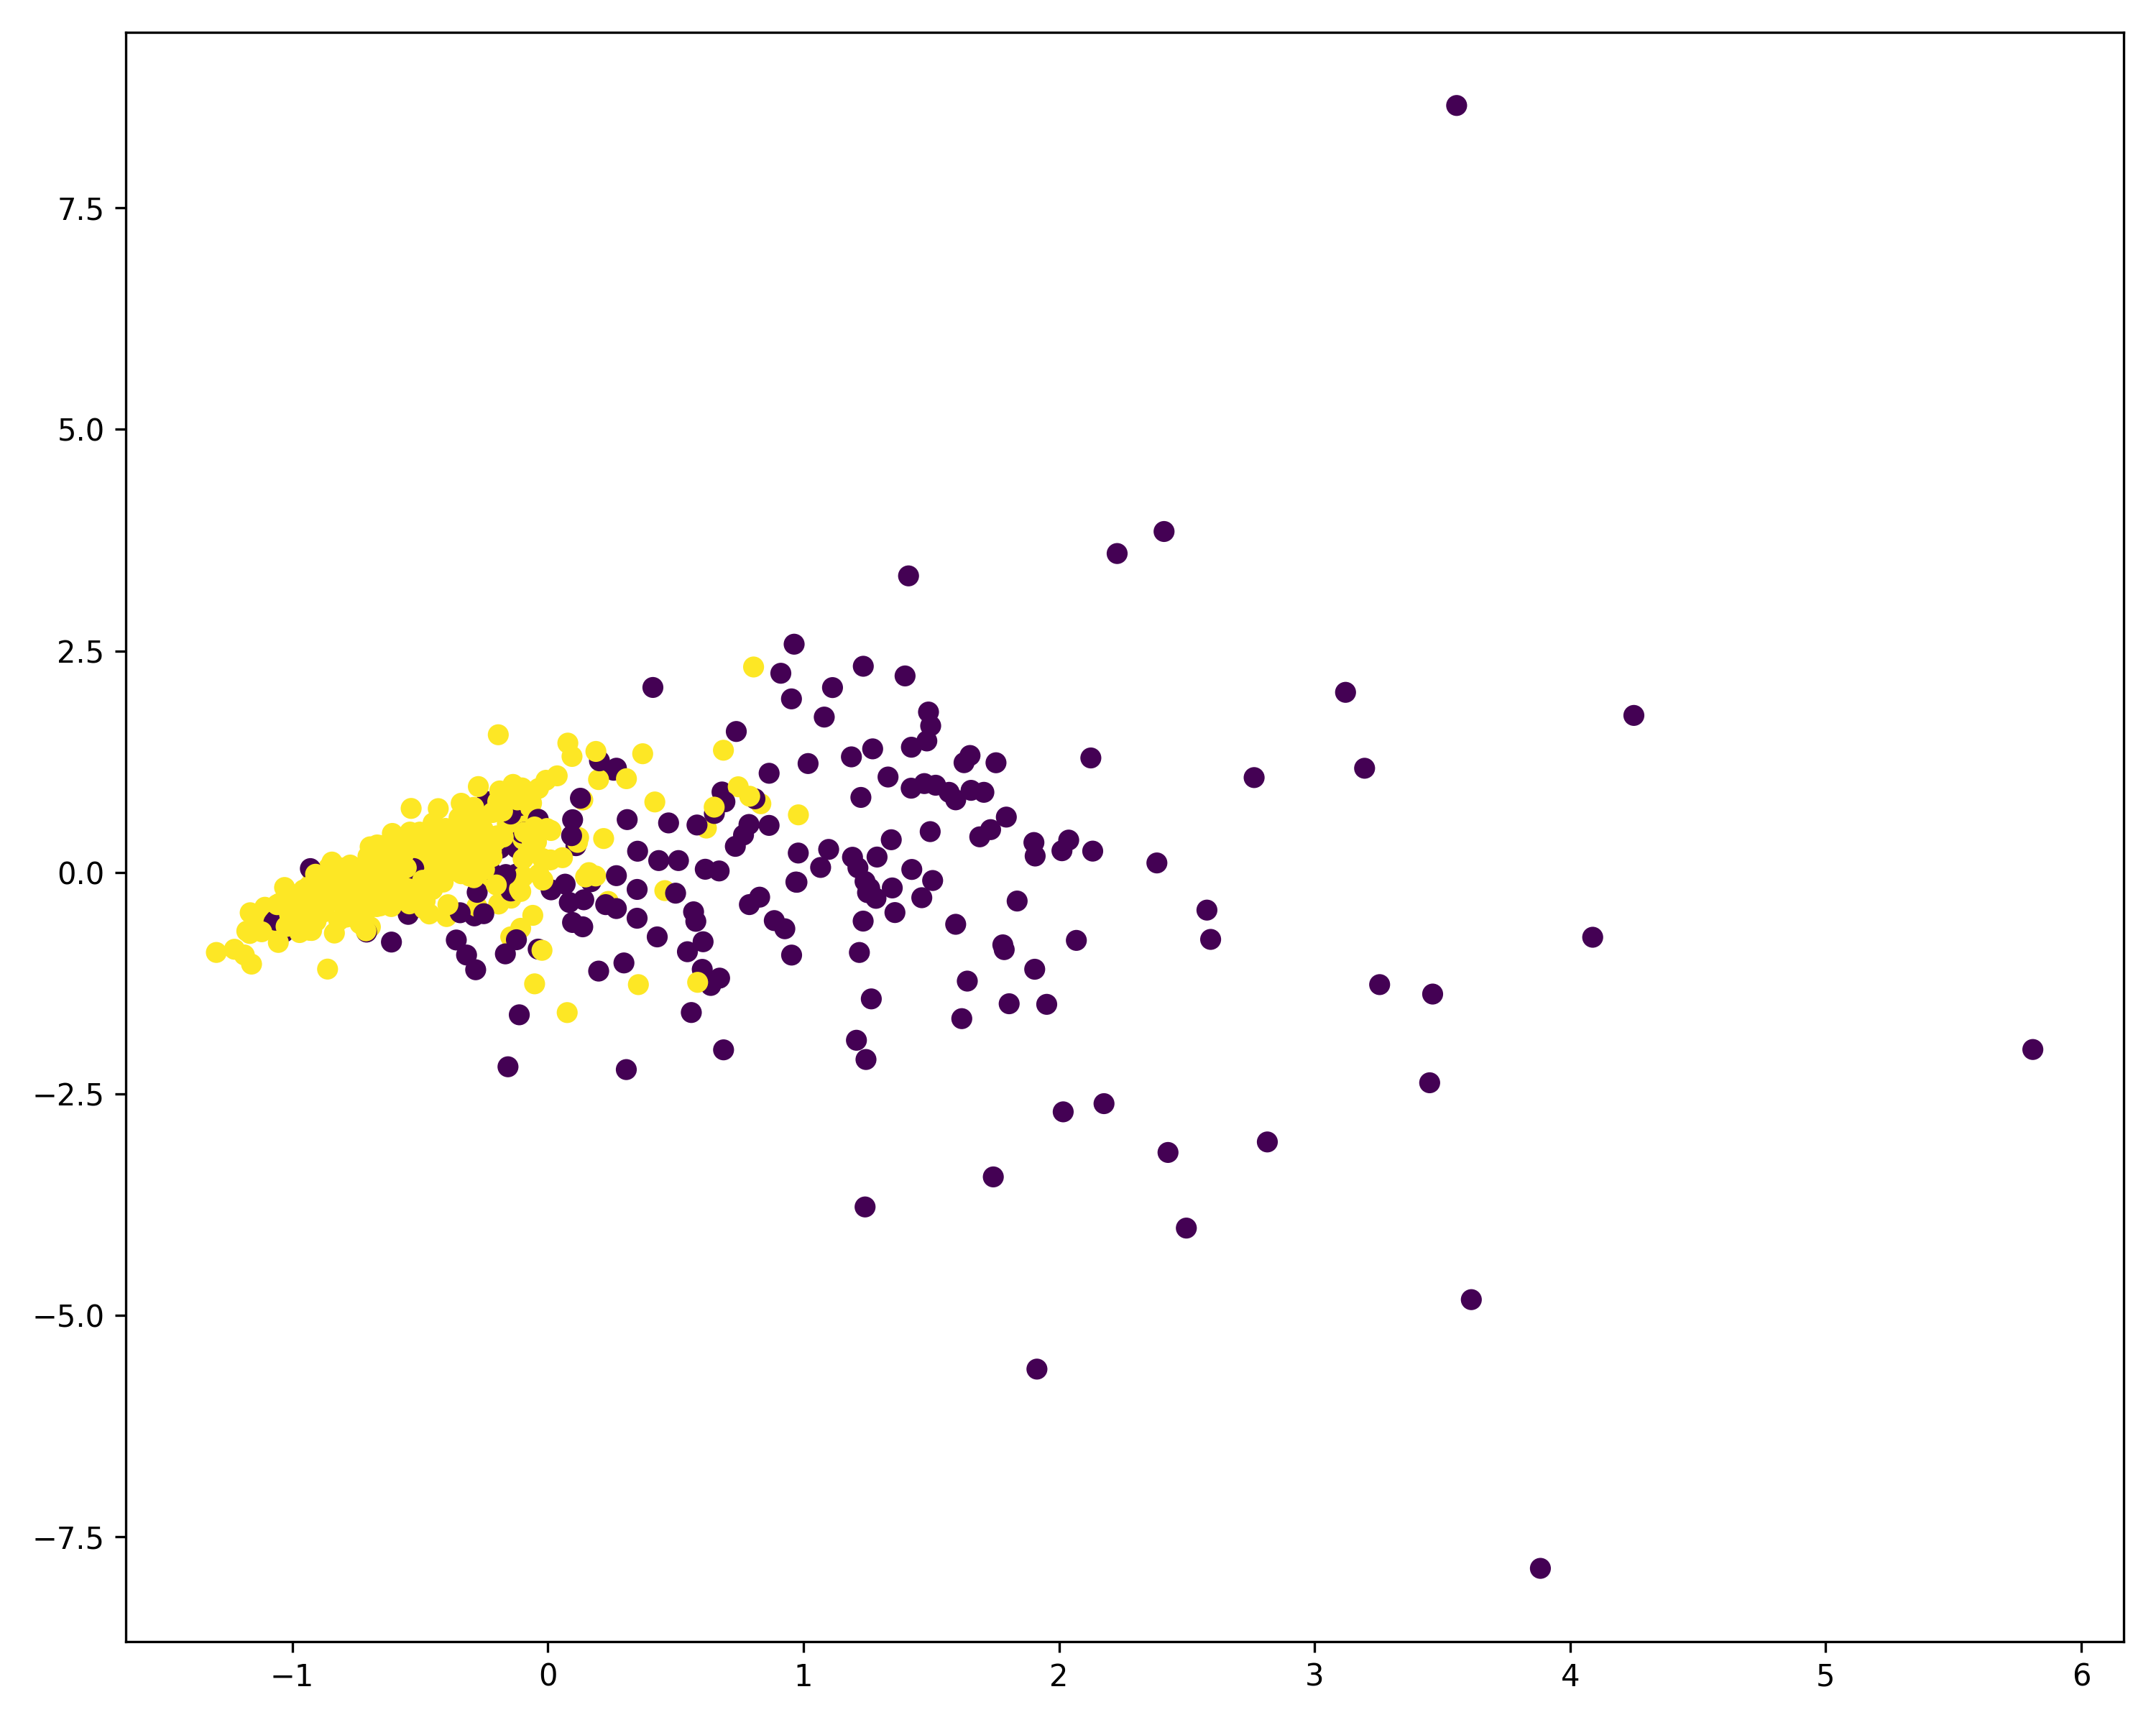
\includegraphics[width=\linewidth]{images/claire/random_n0_breast_cancer_kmeans_n_clusters_2.png}
\end{minipage}
\caption{Partições do K-means, com $K = 3$ (Iris e Wine) e $K = 2$ (Breast Cancer), para conjuntos de dados reais.}
\end{figure}


\begin{figure}
\centering
\begin{minipage}{.4\textwidth}
  \centering
  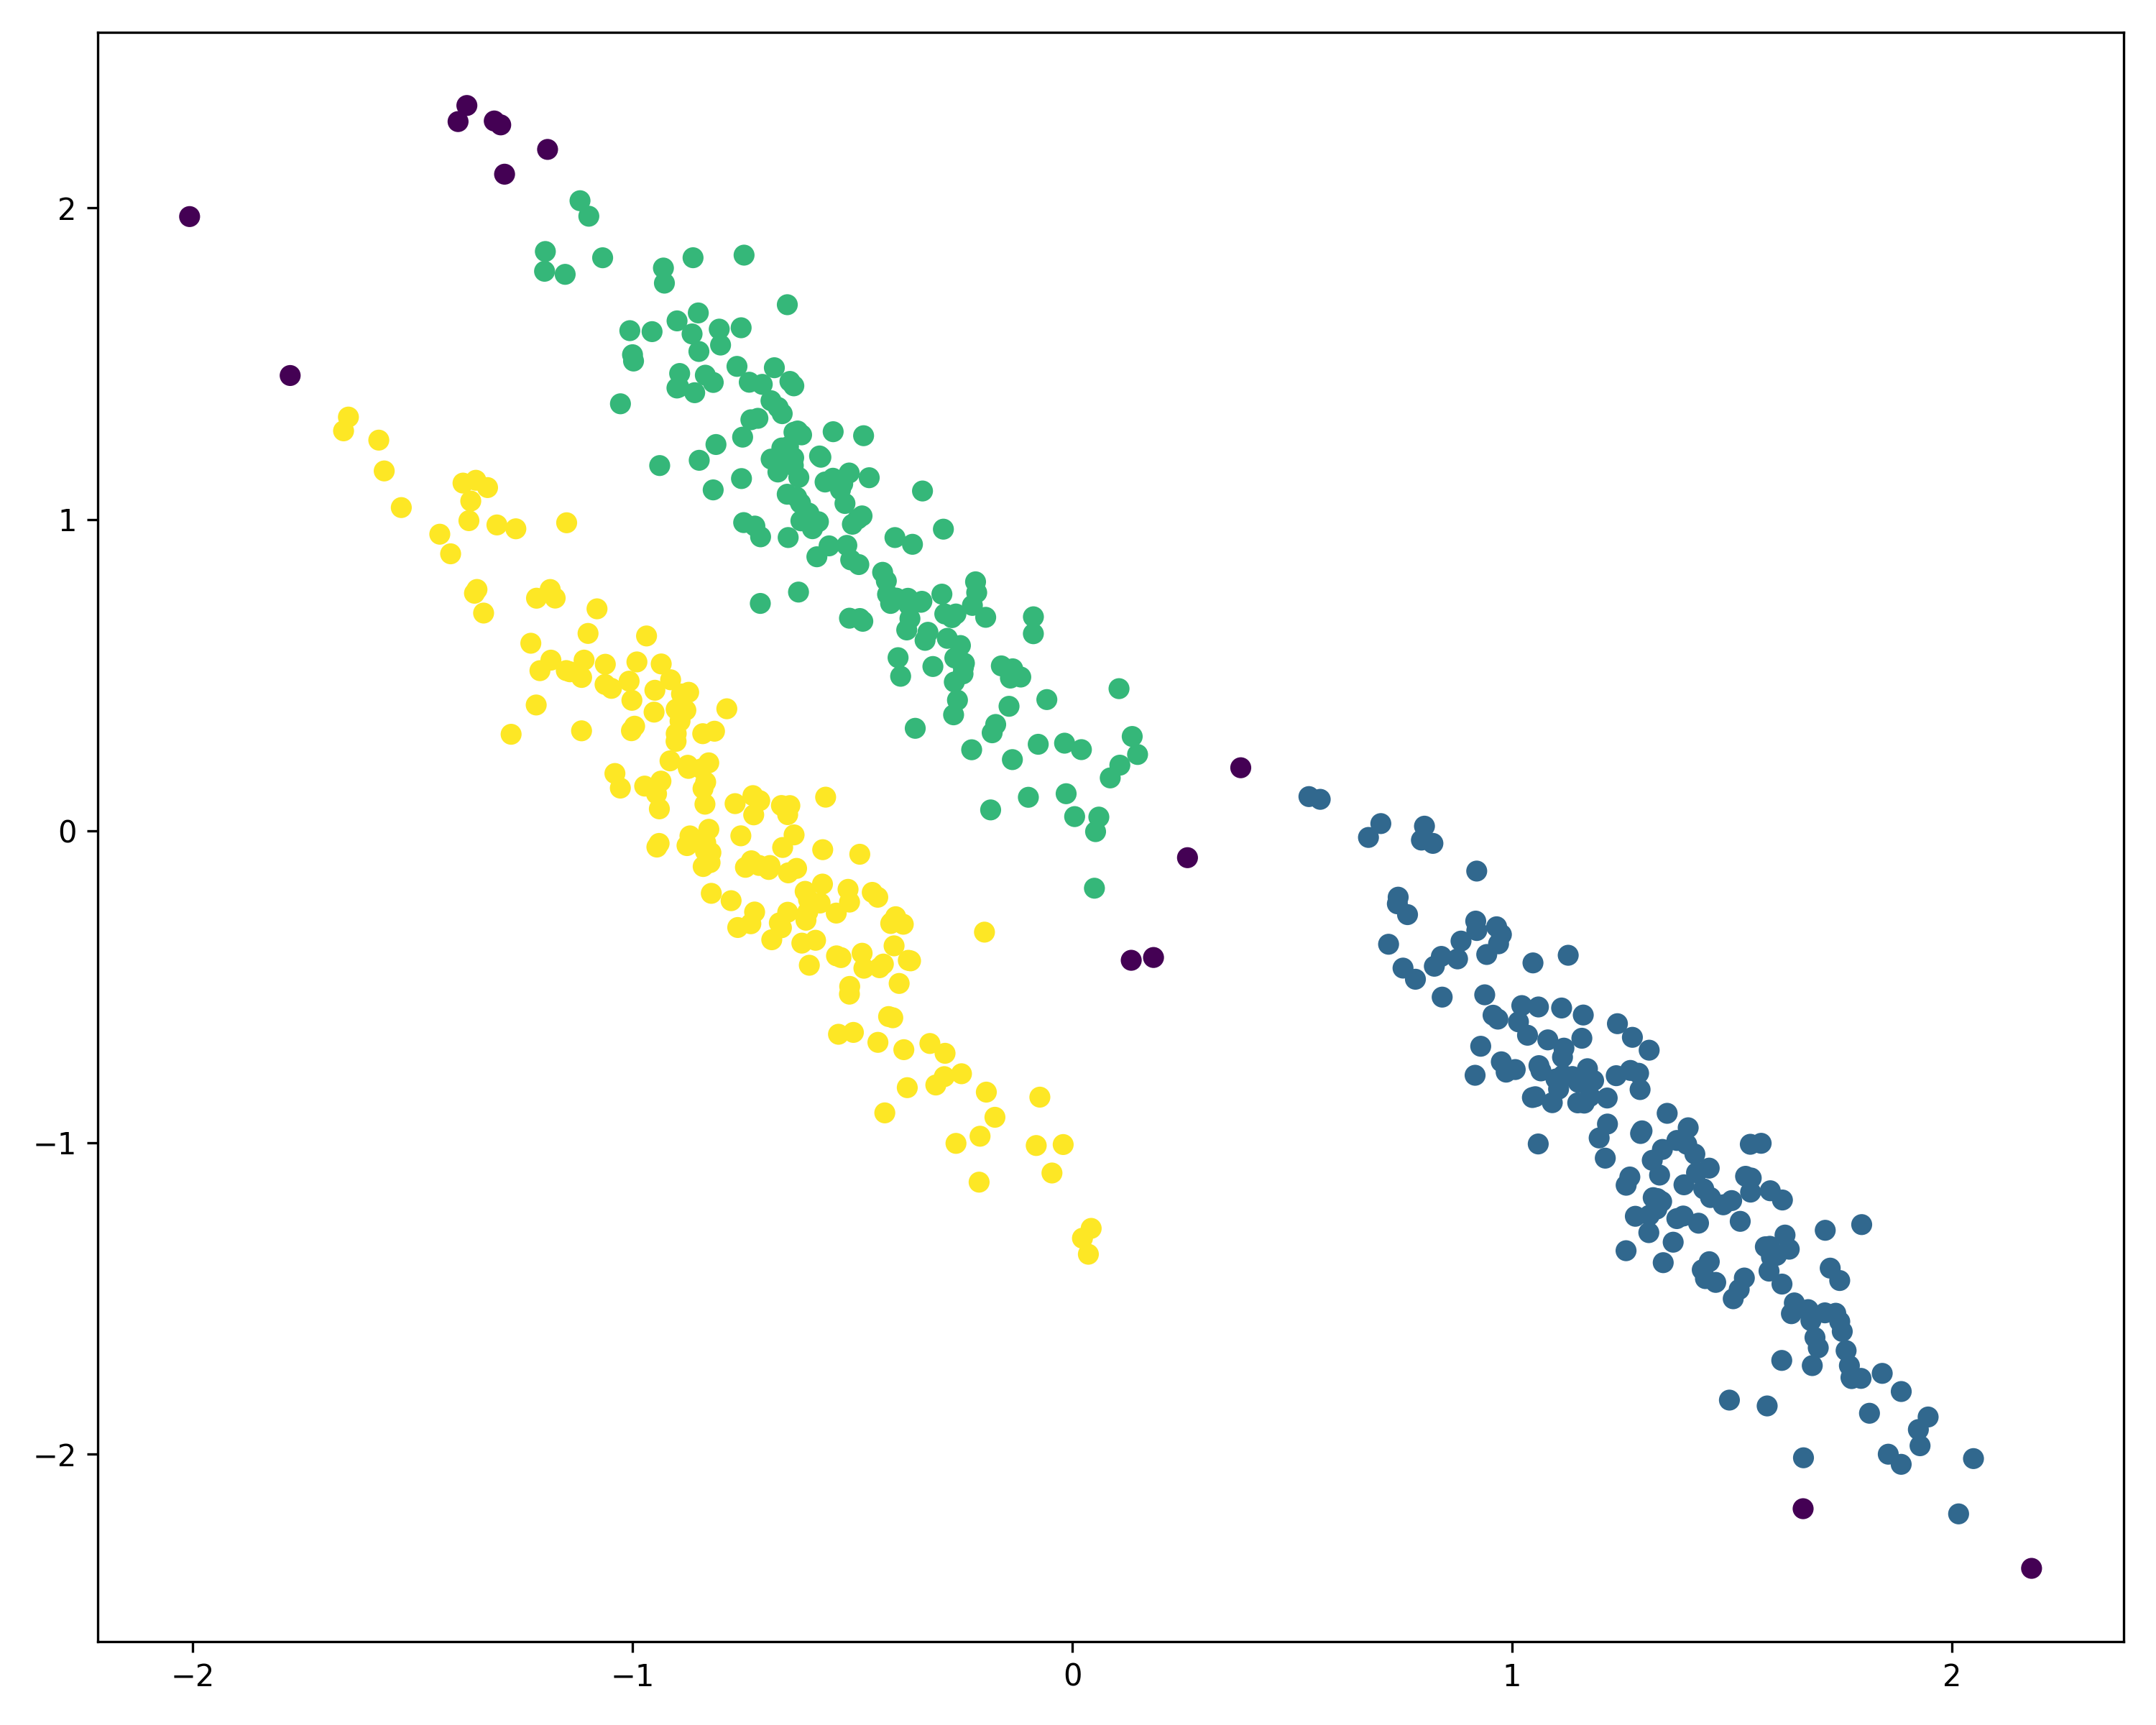
\includegraphics[width=\linewidth]{images/claire/random_n0_aniso_optics_min_samples_7_xi_0_1_min_cluster_size_0_2.png}
\end{minipage}%
\hspace{0.02cm}
\begin{minipage}{.4\textwidth}
  \centering
  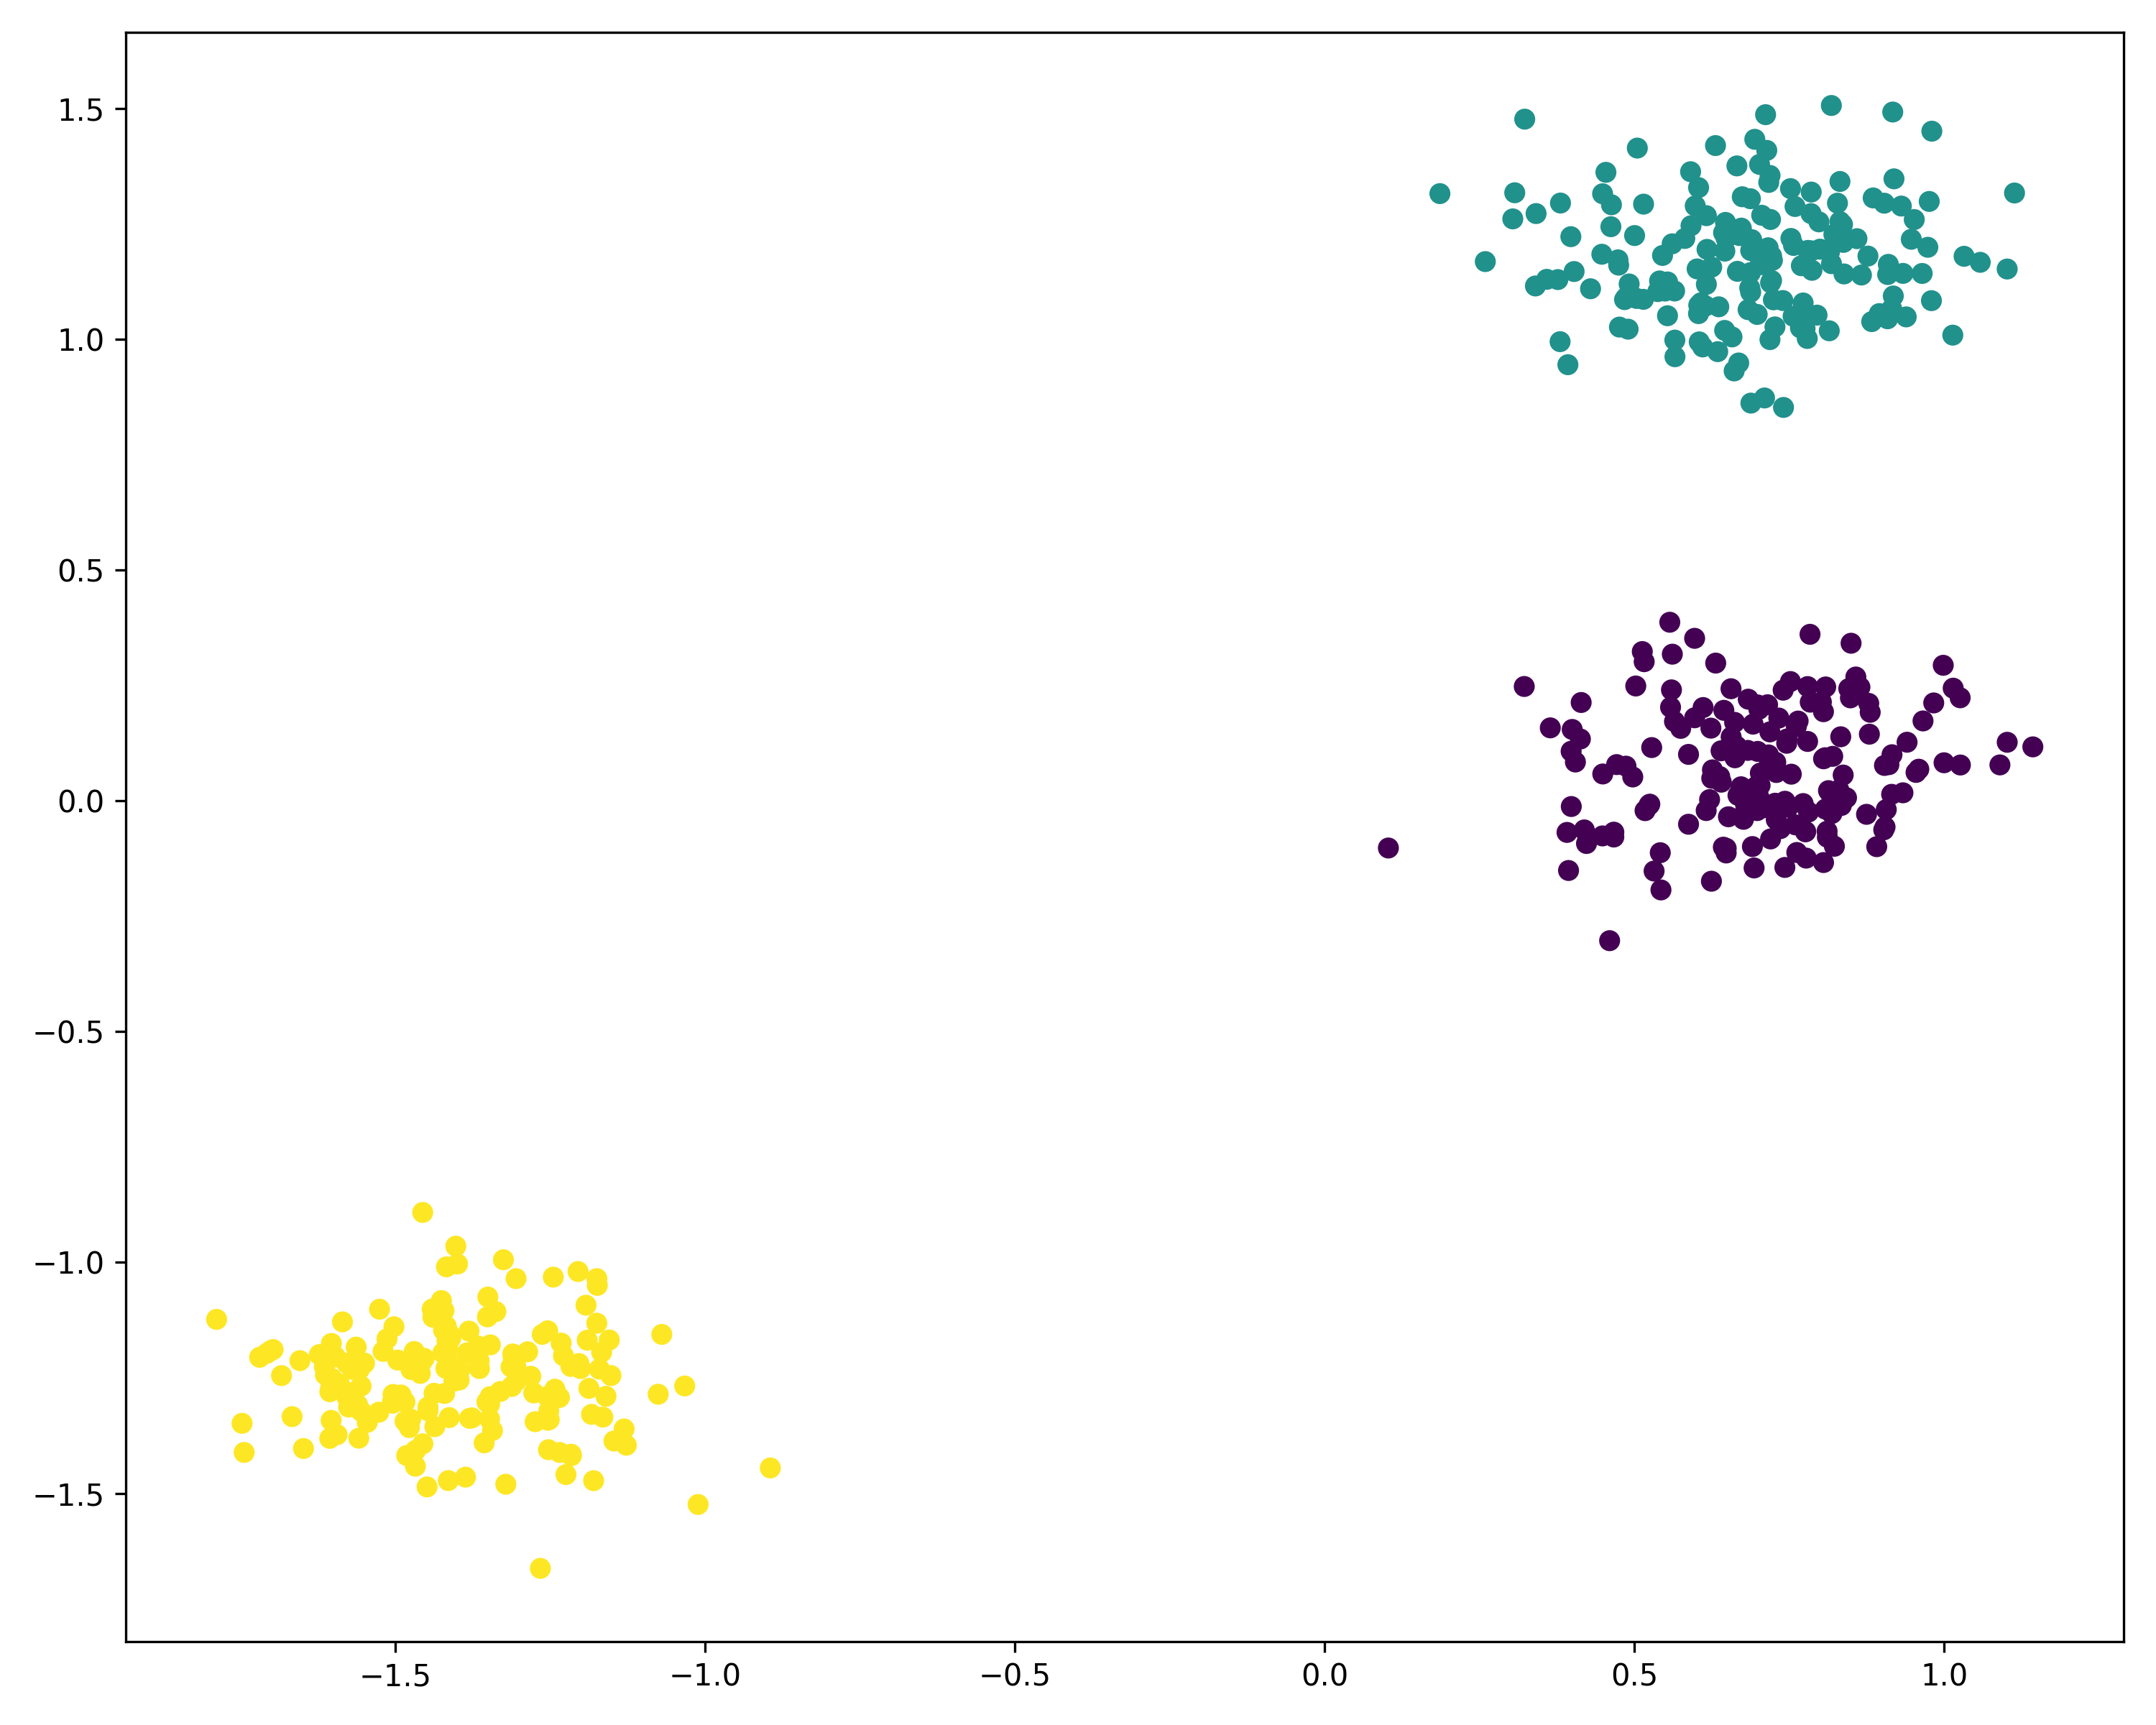
\includegraphics[width=\linewidth]{images/claire/random_n0_blobs_mean_shift_.png}
\end{minipage}
\vspace{0.02cm}
\begin{minipage}{.4\textwidth}
  \centering
  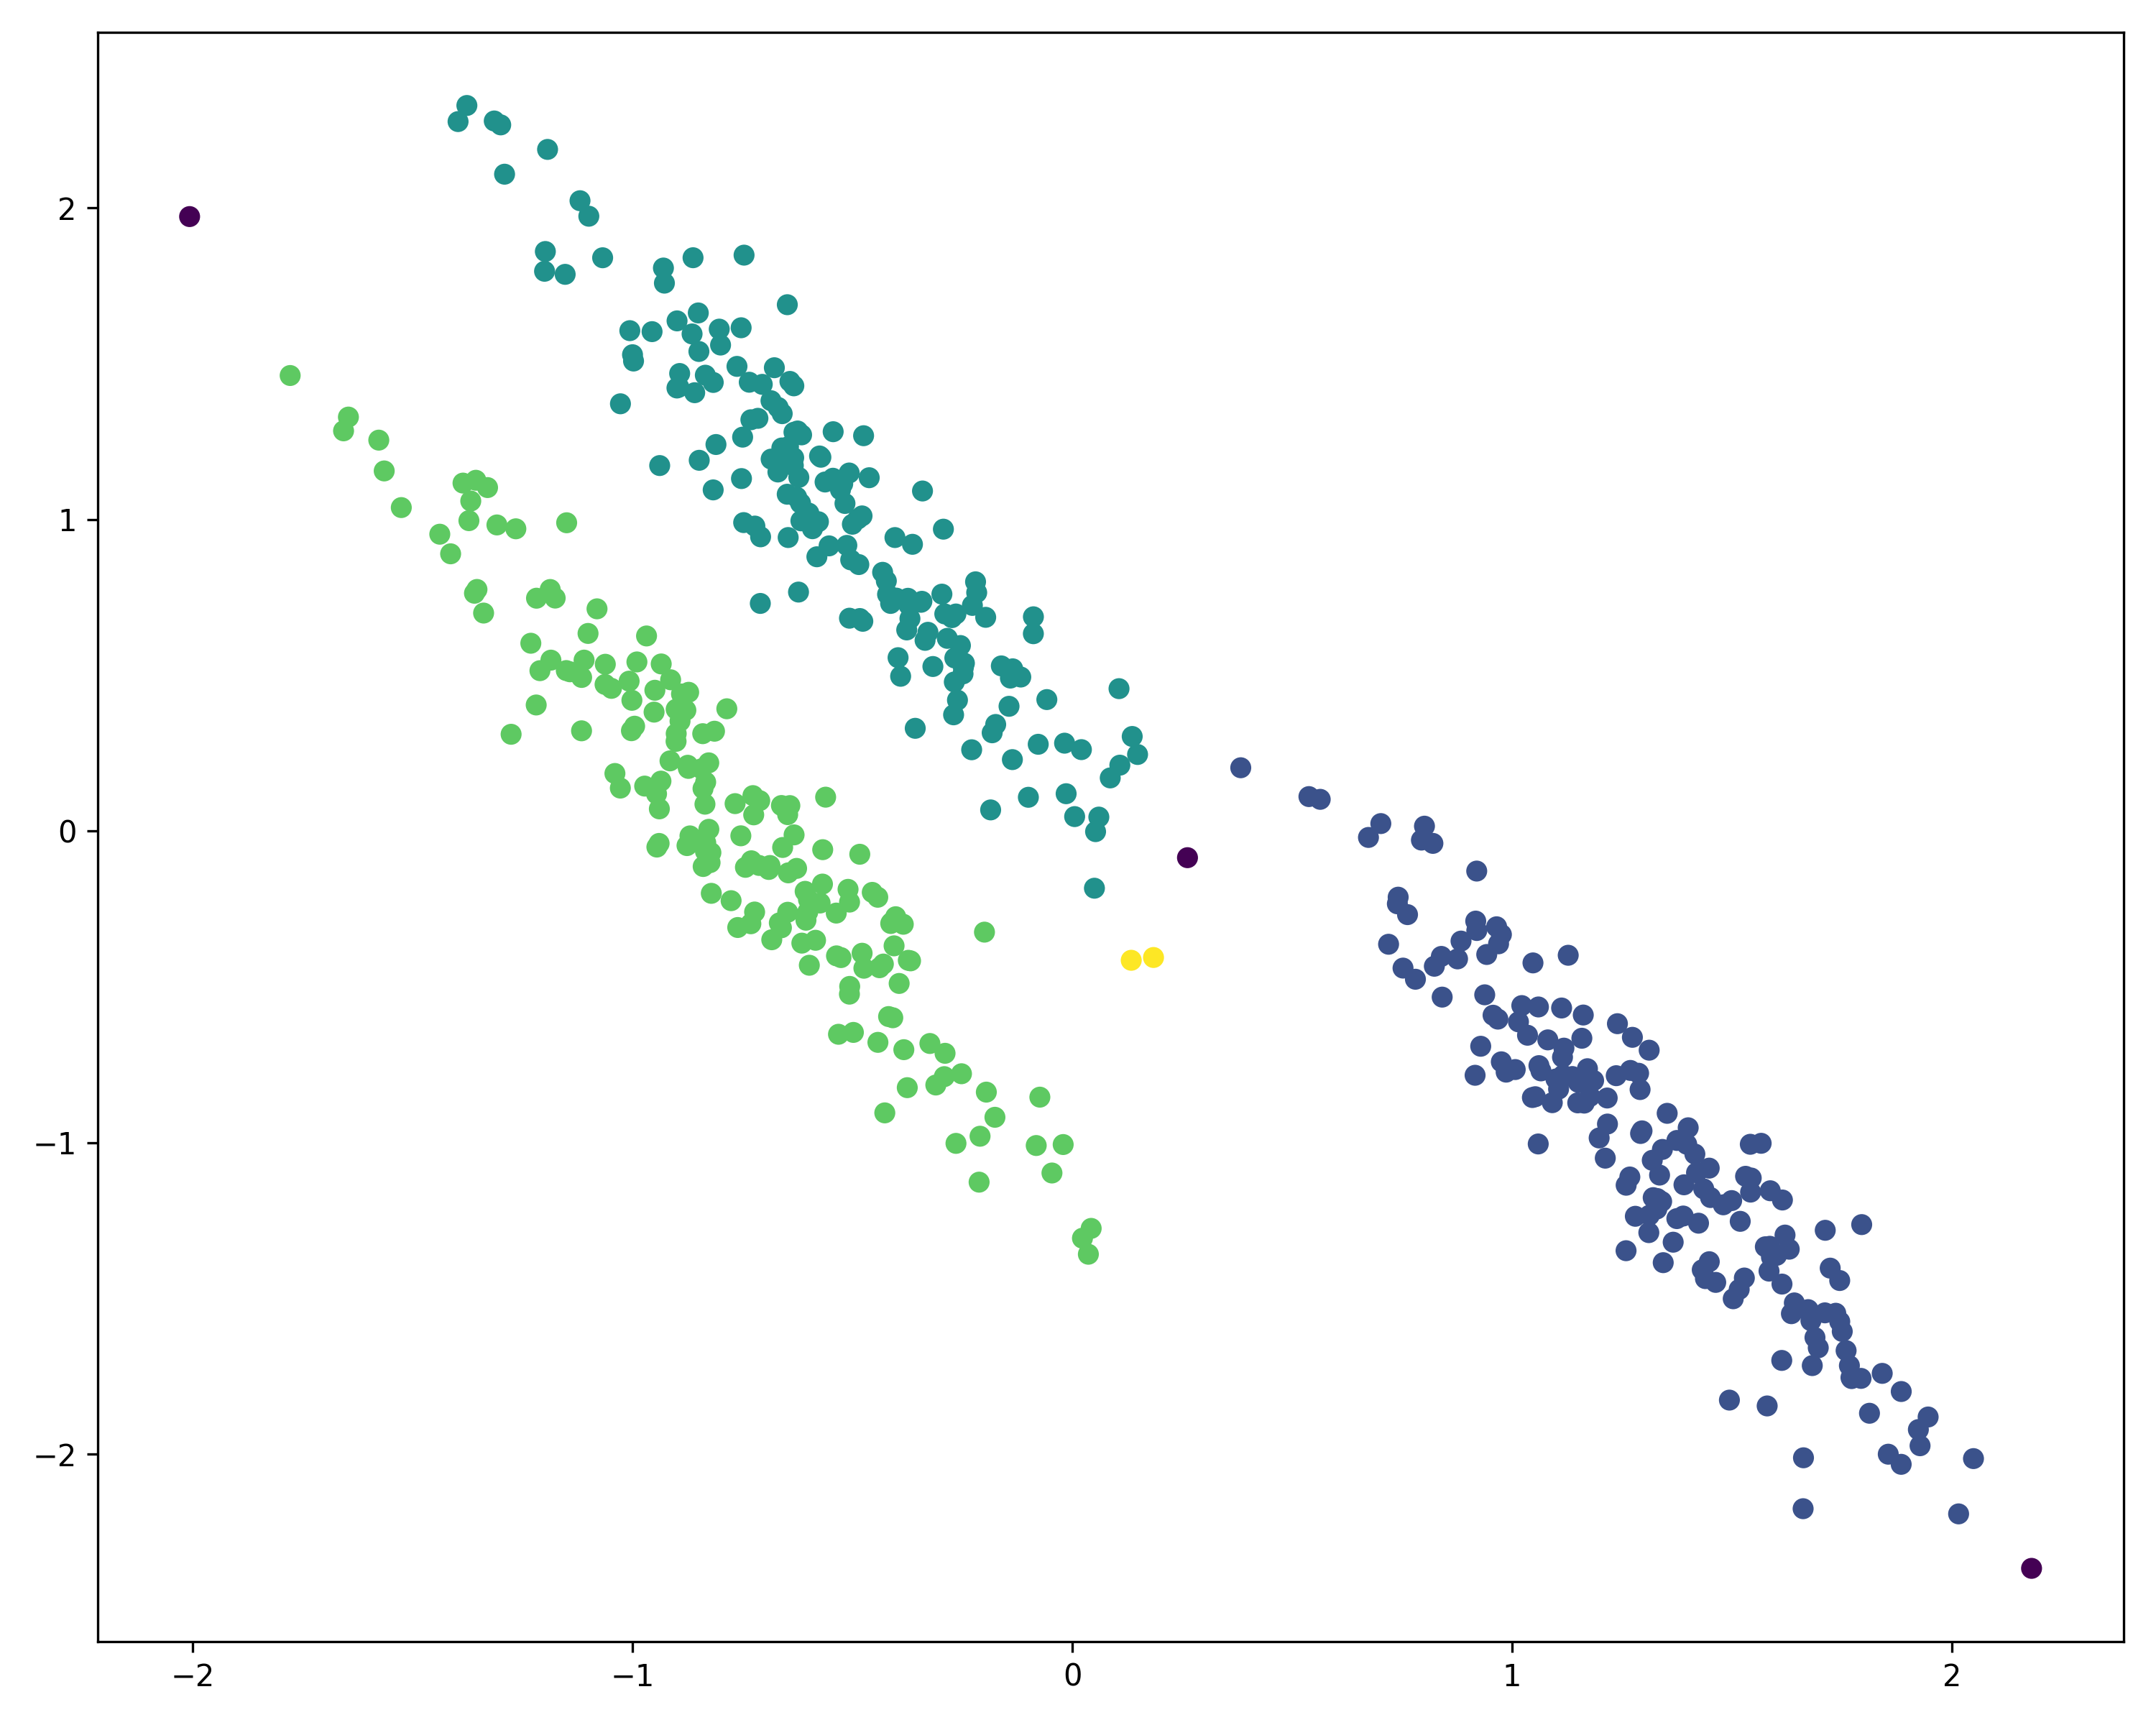
\includegraphics[width=\linewidth]{images/claire/random_n0_aniso_dbscan_eps_0_2_min_samples_2.png}
\end{minipage}%
\hspace{0.02cm}
\begin{minipage}{.4\textwidth}
  \centering
  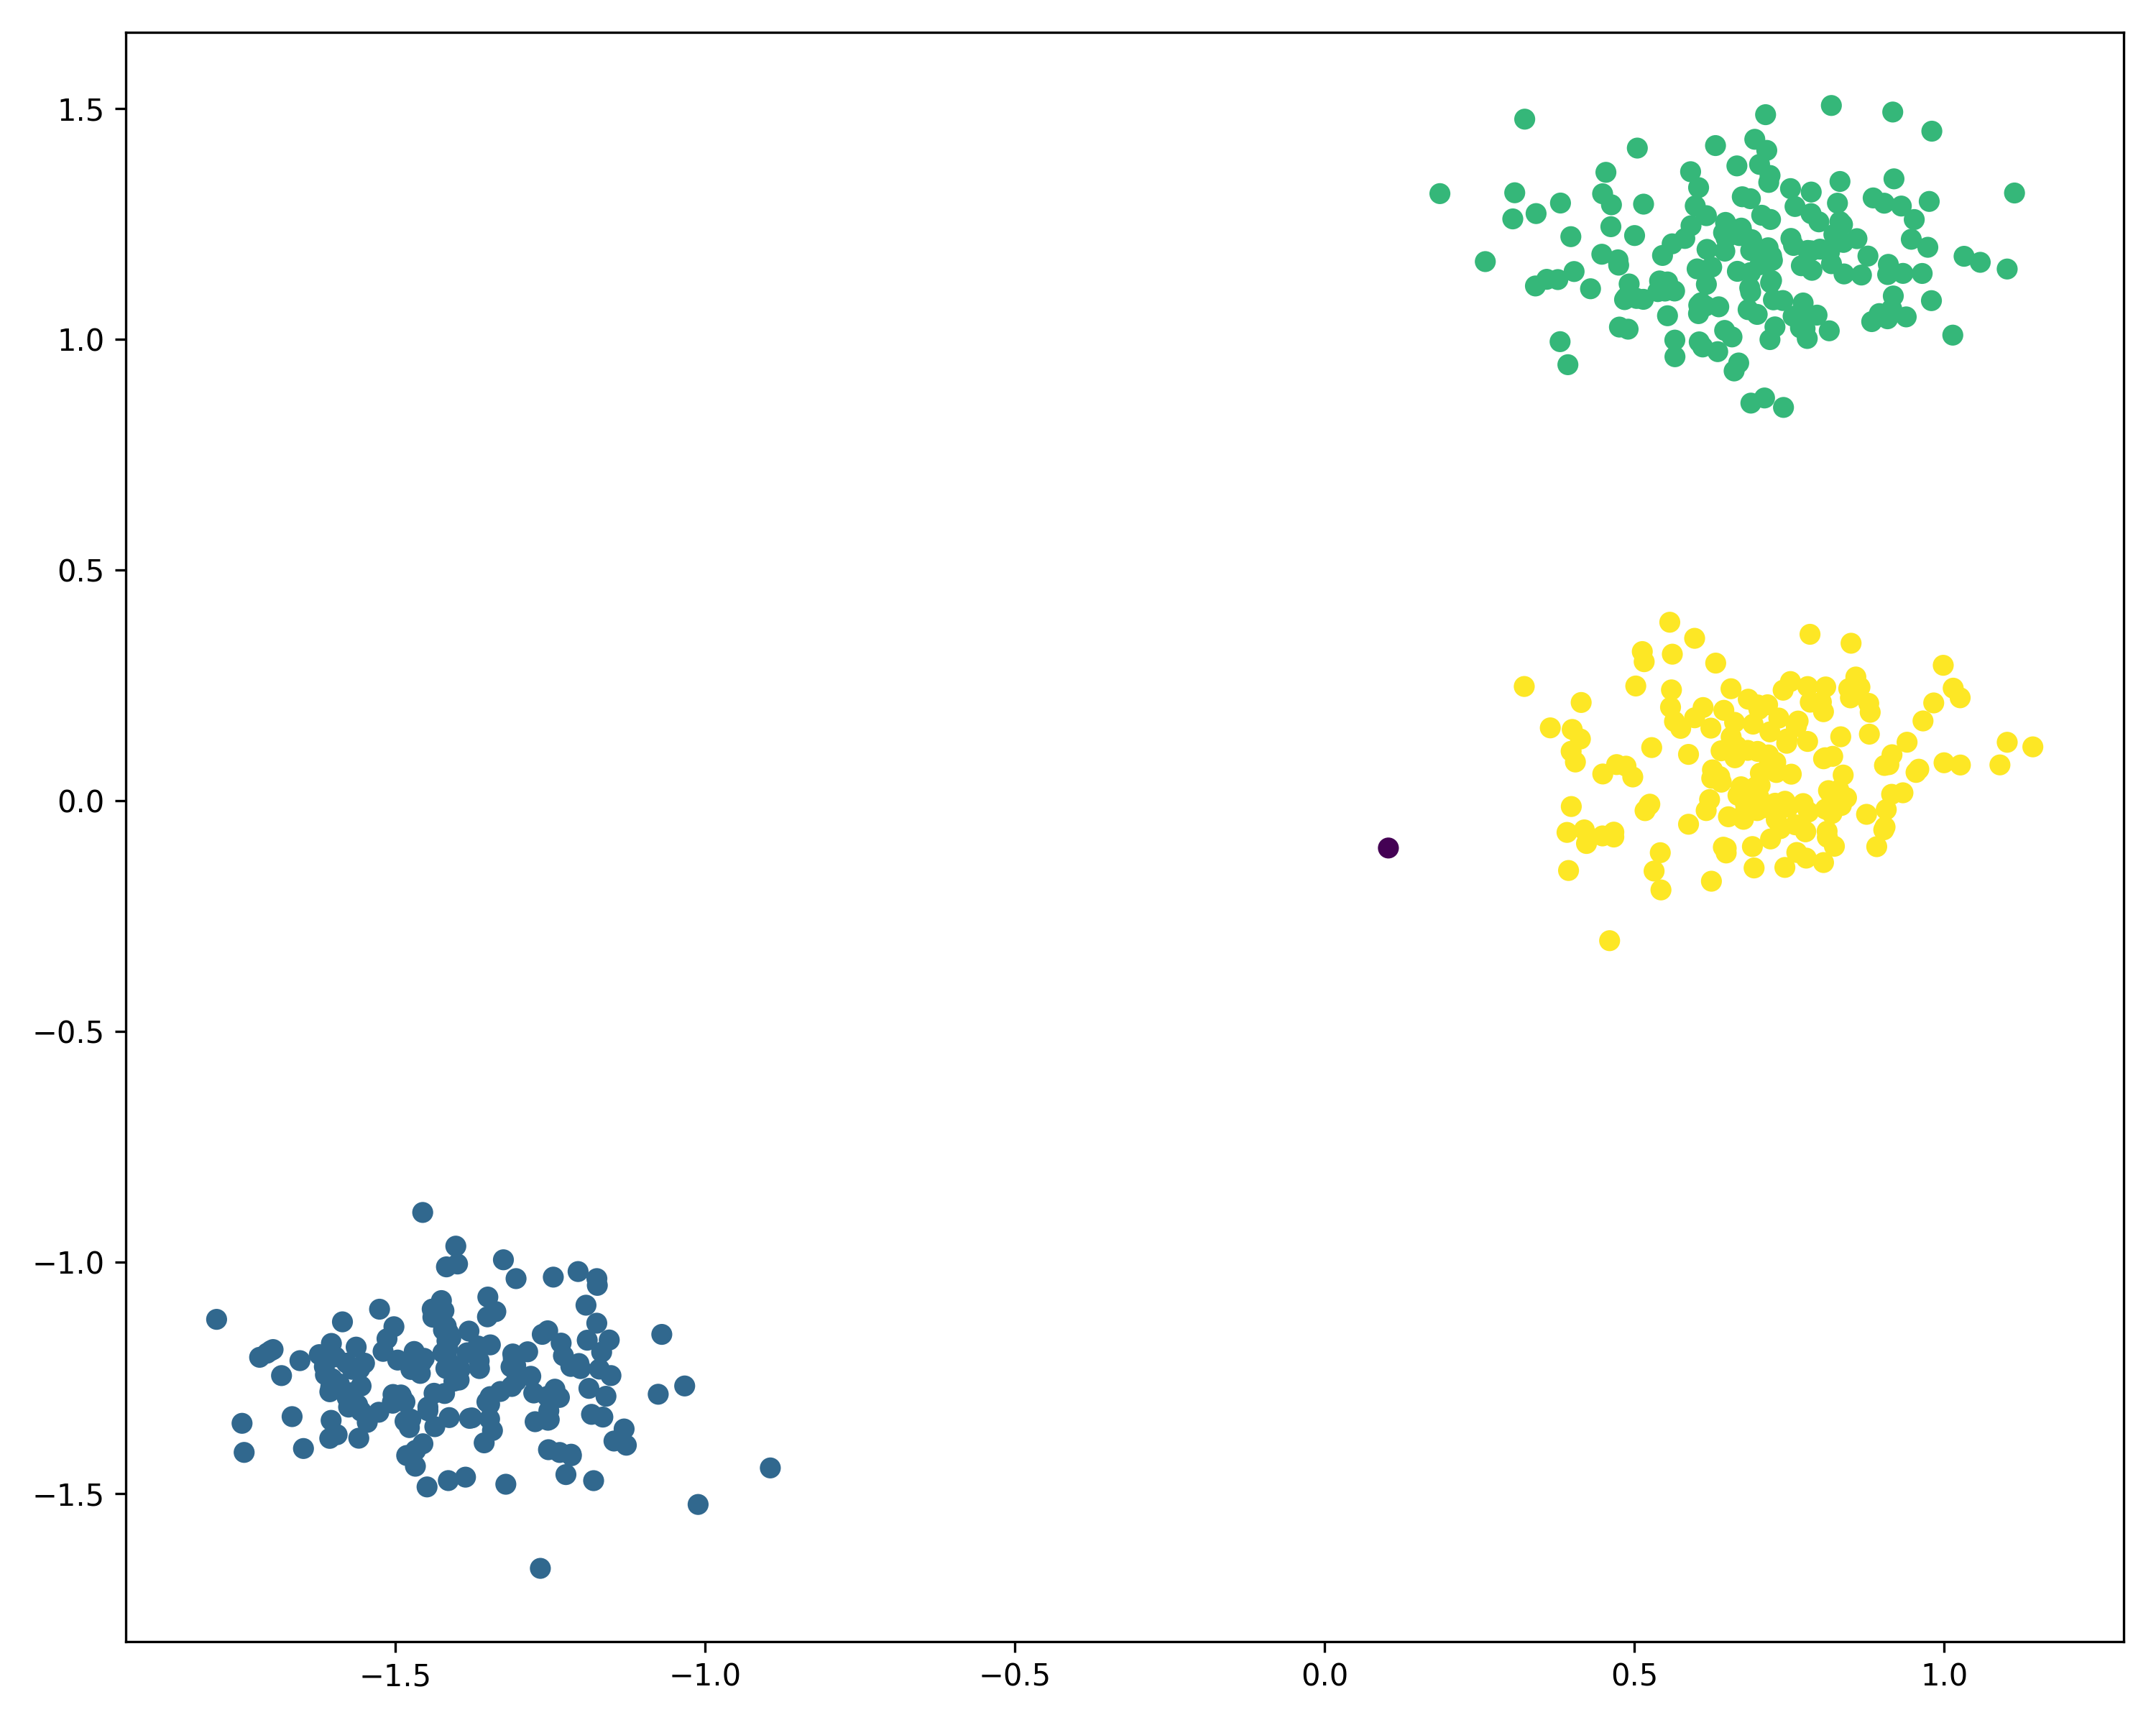
\includegraphics[width=\linewidth]{images/claire/random_n0_blobs_dbscan_eps_0_2_min_samples_2.png}
\end{minipage}
\begin{minipage}{.4\textwidth}
  \centering
  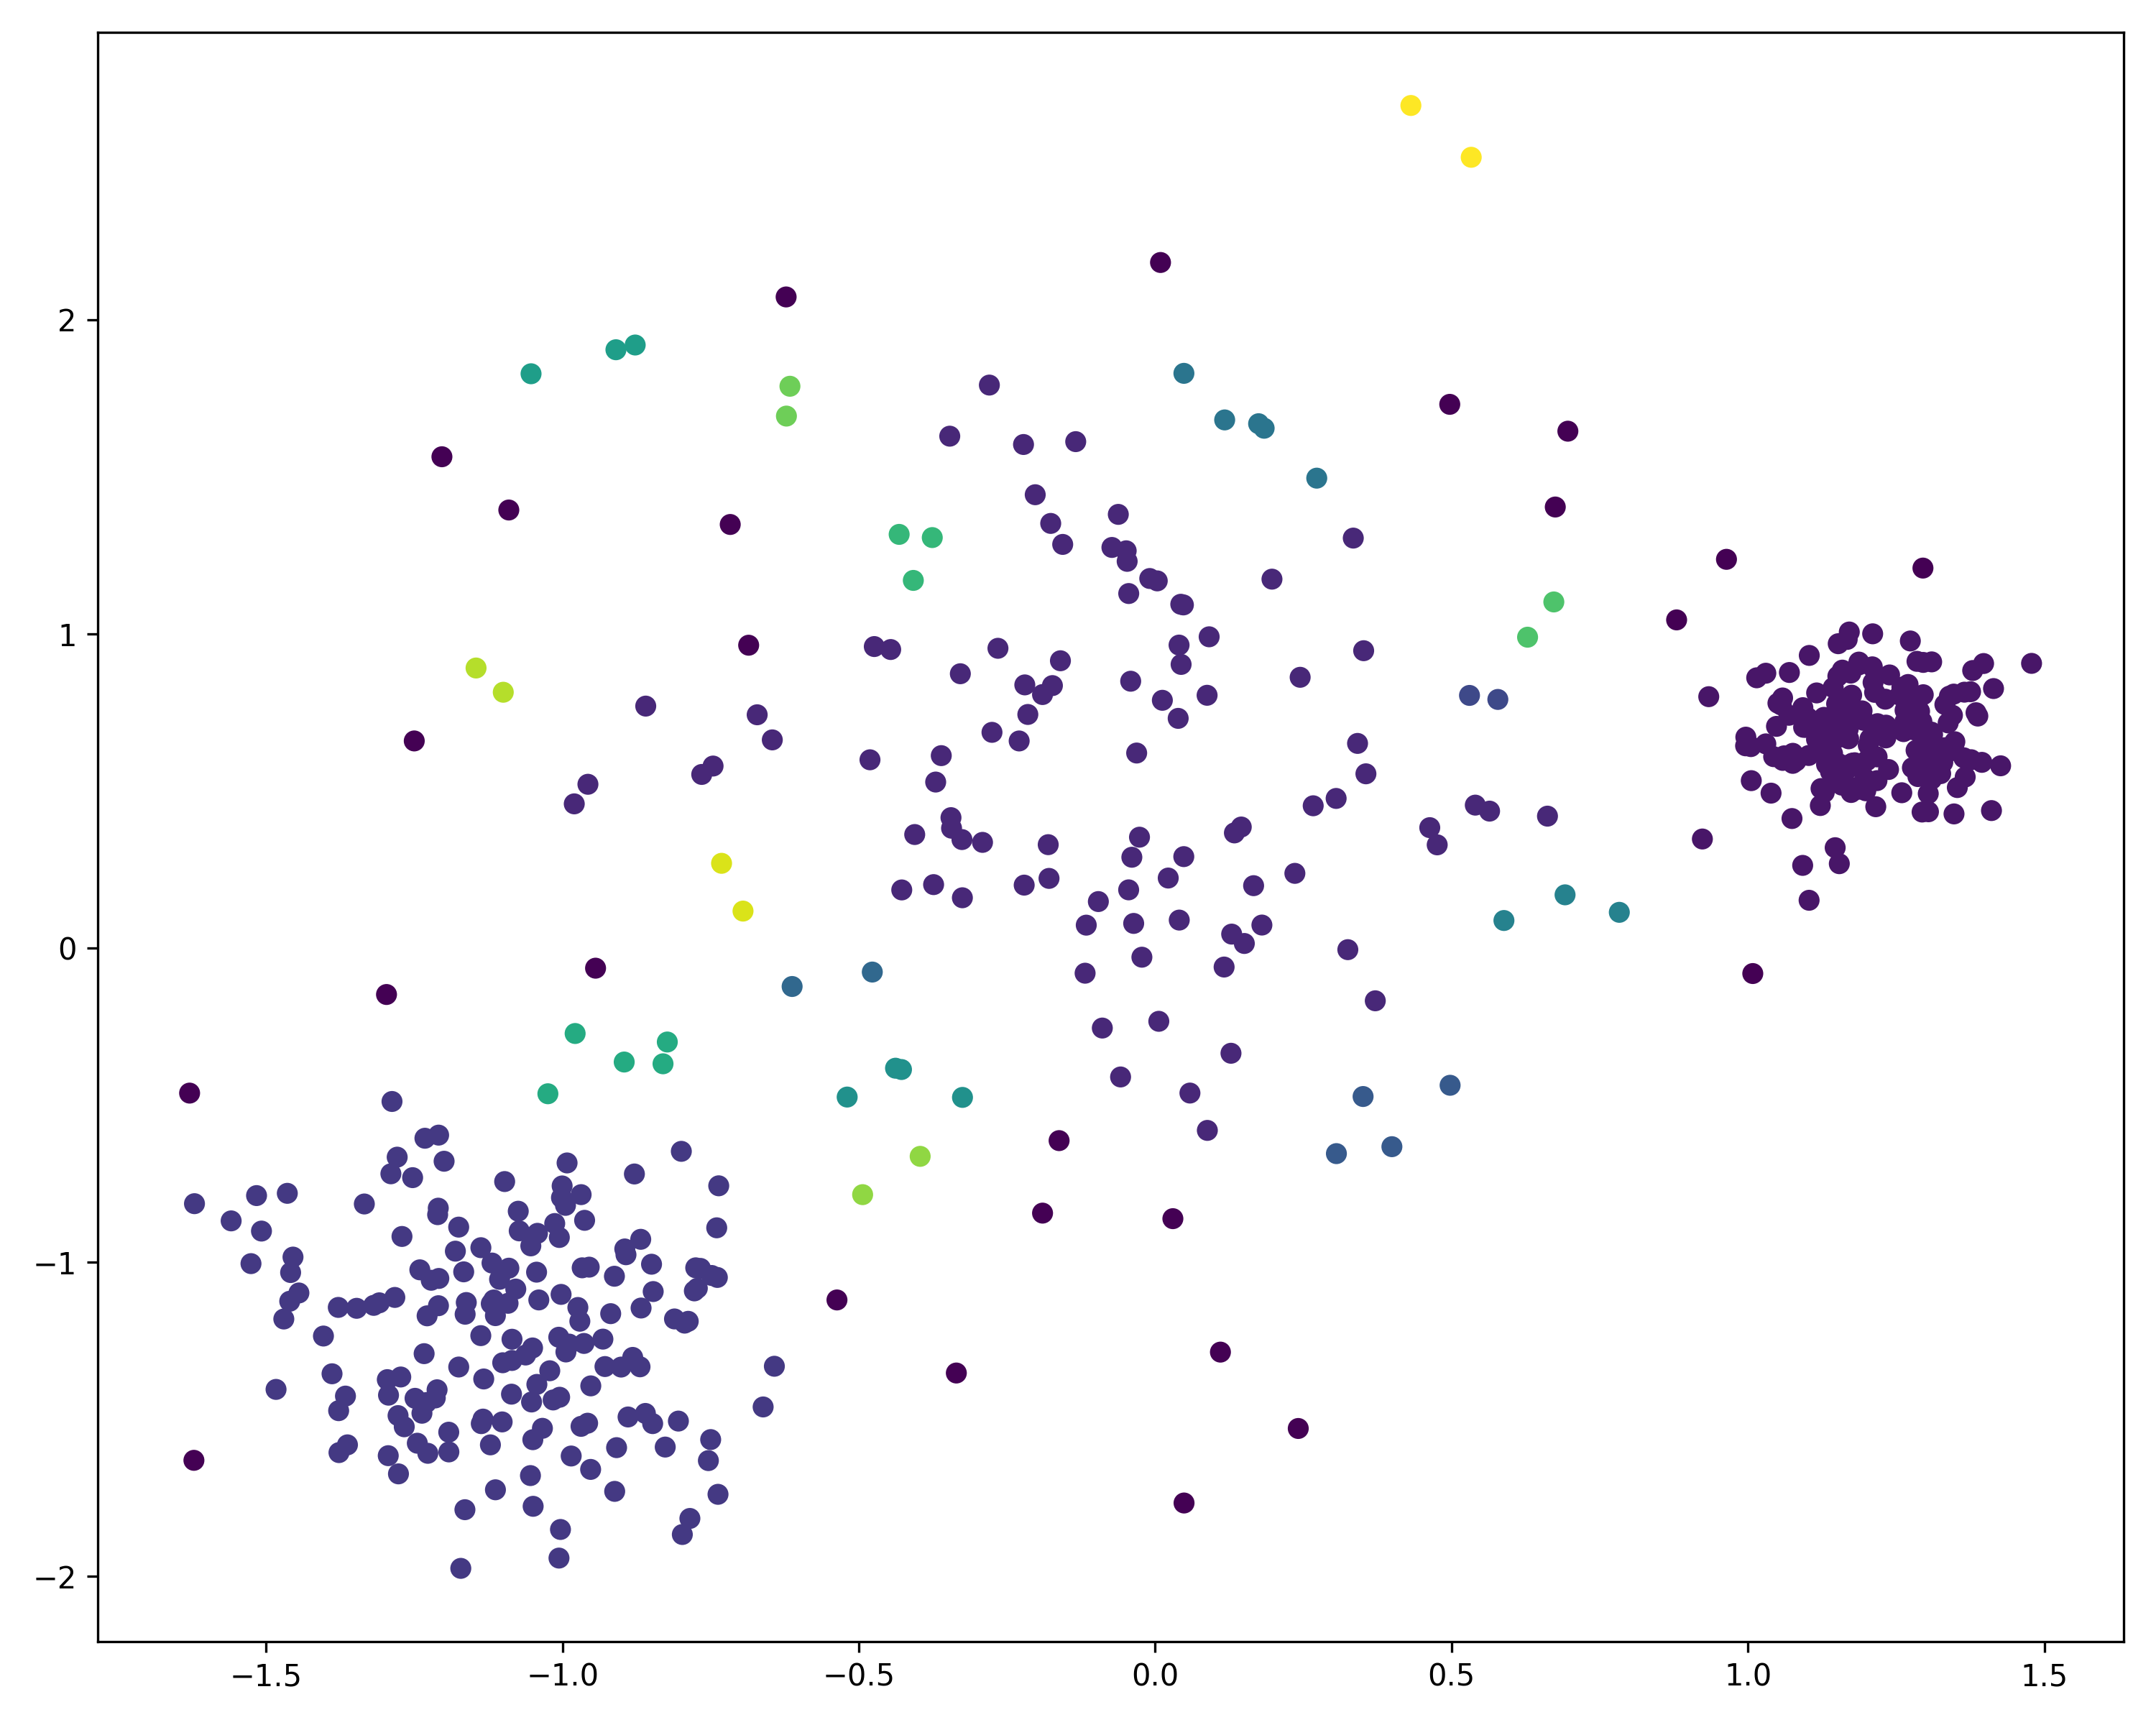
\includegraphics[width=\linewidth]{images/claire/random_n0_varied_dbscan_eps_0_2_min_samples_2.png}
\end{minipage}
\caption{Partições que encontraram corretamente o número de clusters, pelo DBSCAN com $\epsilon = 0.2$ (Aniso, Blobs e Varied), OPTICS com \textsf{min\_samples} = $7$, \textsf{xi} = $0.1$, \textsf{min\_cluster\_size} = $0.2$ (Aniso) e Mean Shift (Blobs).}

\end{figure}

\begin{figure}[t]
\centering
\begin{minipage}{.3\textwidth}
  \centering
  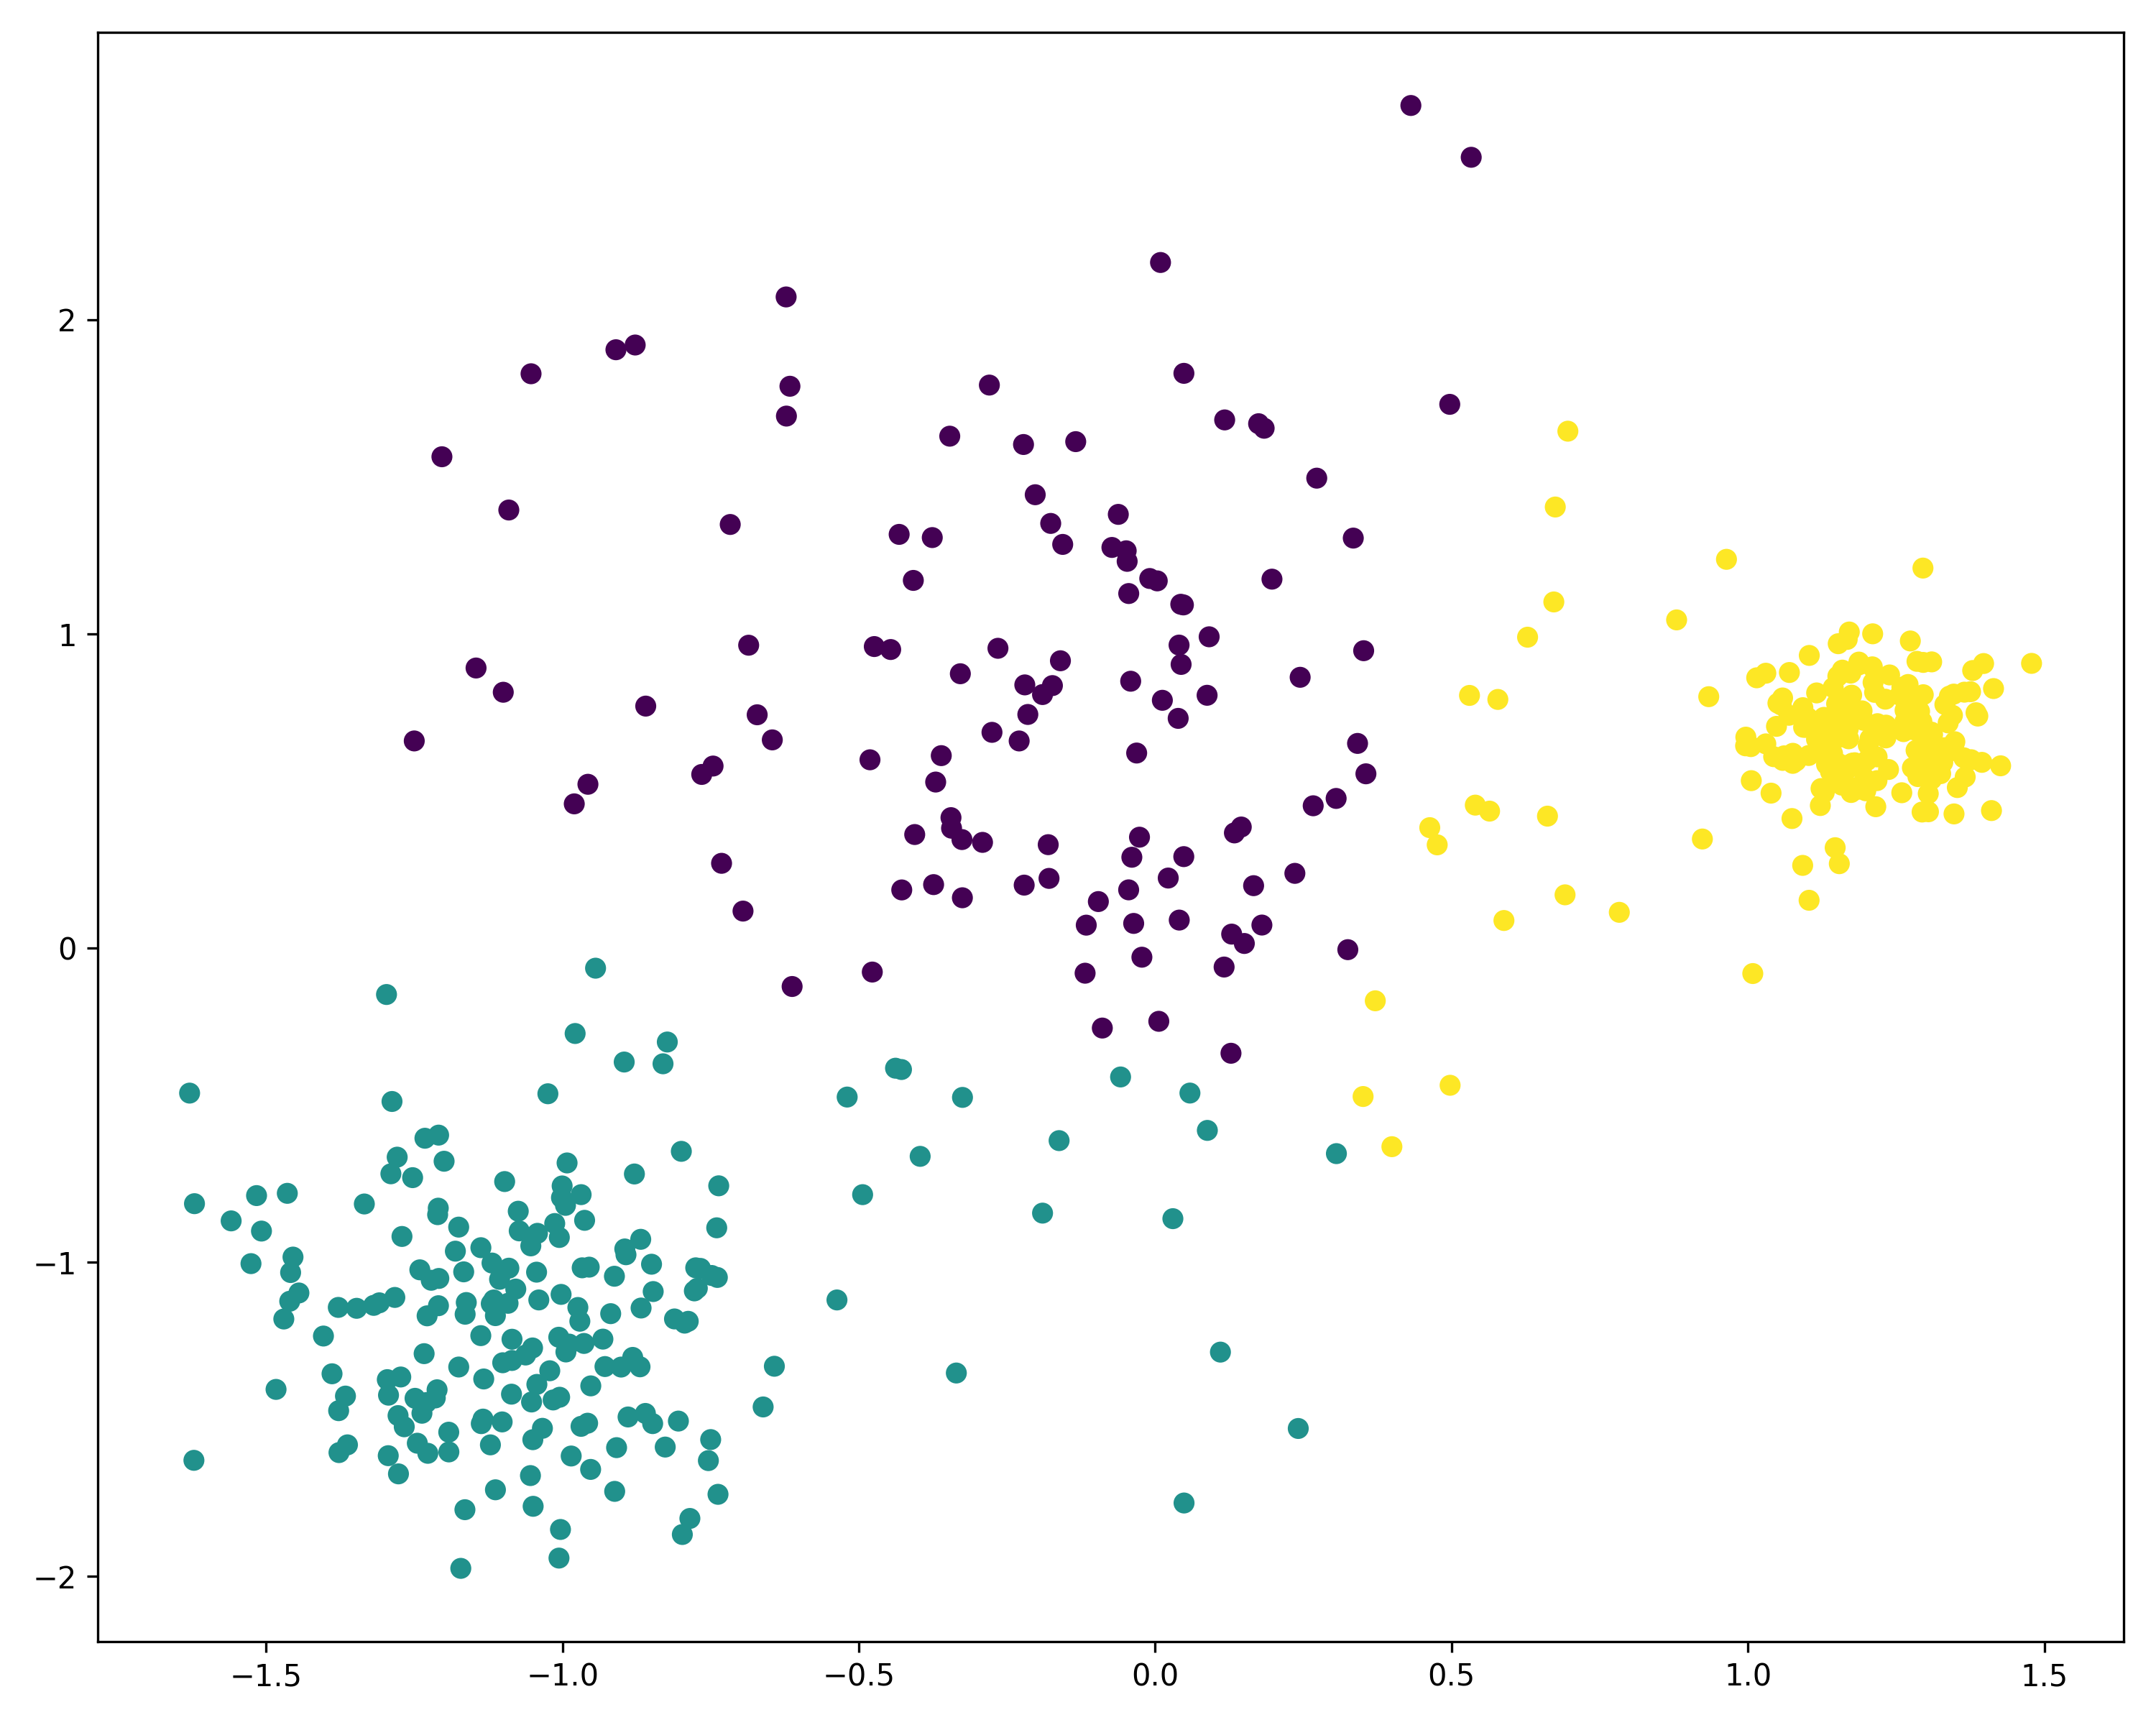
\includegraphics[width=\linewidth]{images/claire/random_n0_varied_kmeans_n_clusters_3.png}
\end{minipage}%
\hspace{0.02cm}
\begin{minipage}{.3\textwidth}
  \centering
  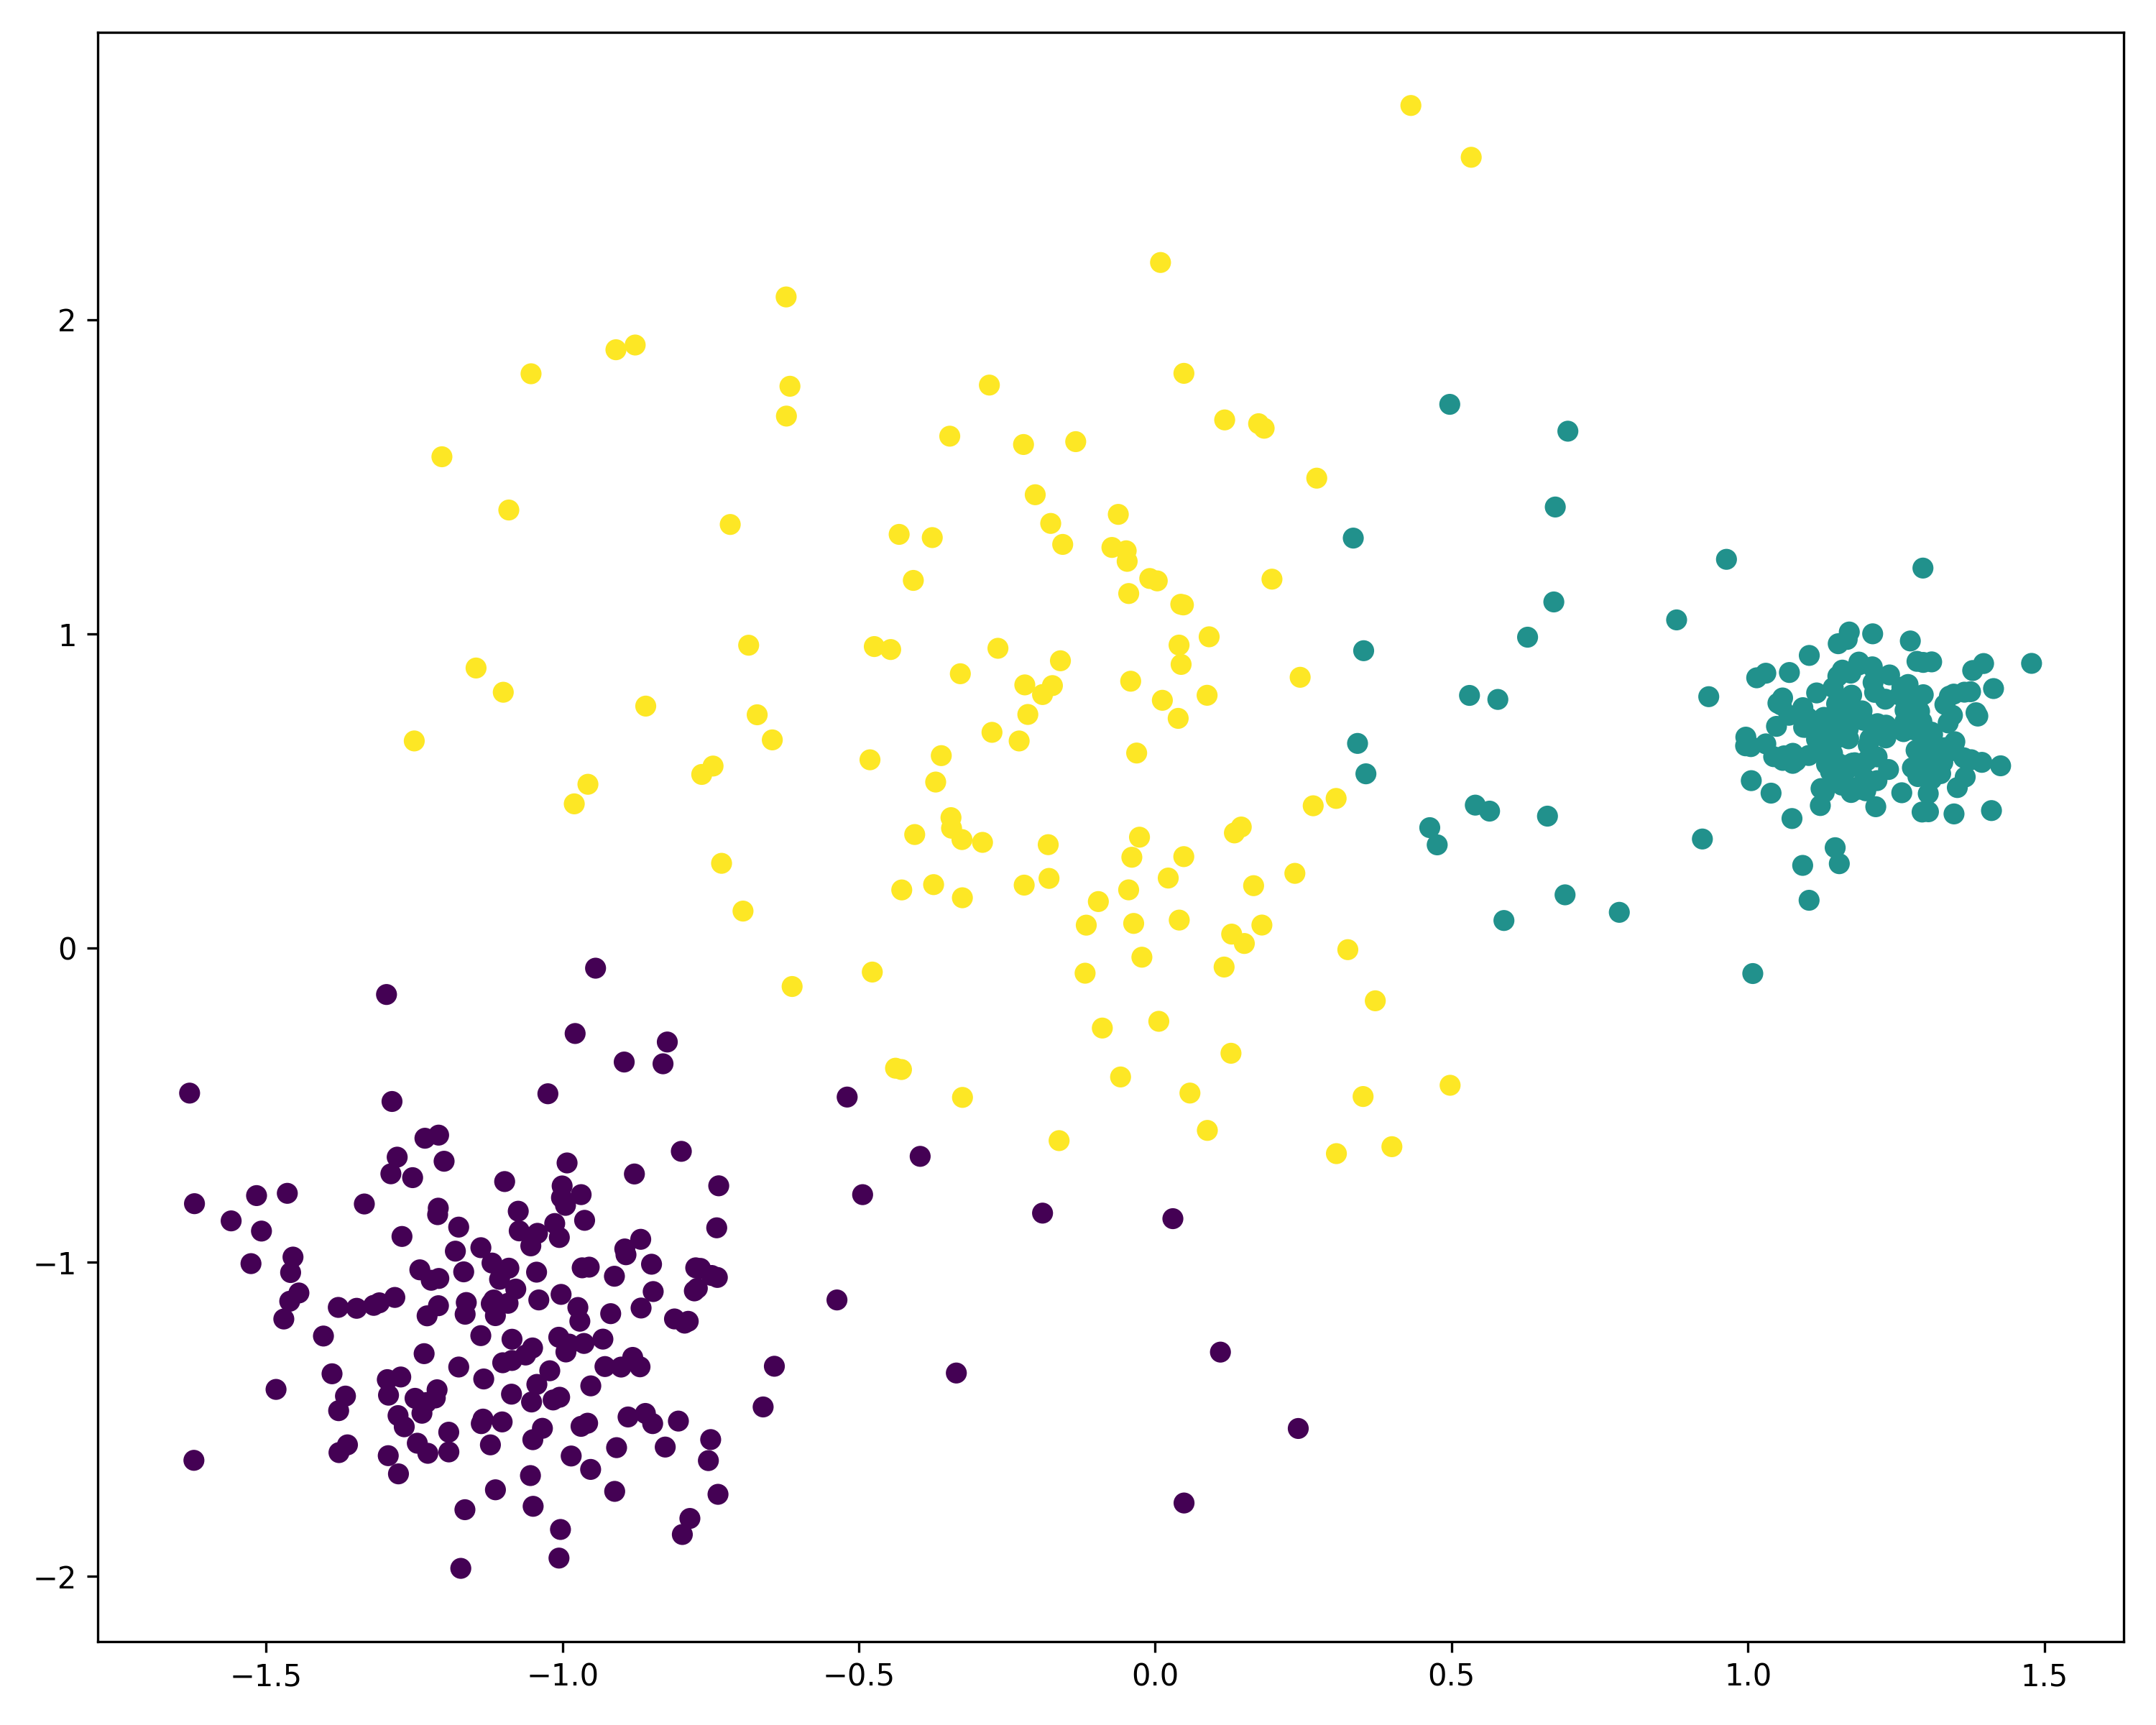
\includegraphics[width=\linewidth]{images/claire/random_n0_varied_kernel_kmeans_n_clusters_3_kernel_gak_random_state_0.png}
\end{minipage}
\hspace{0.02cm}
\begin{minipage}{.3\textwidth}
  \centering
  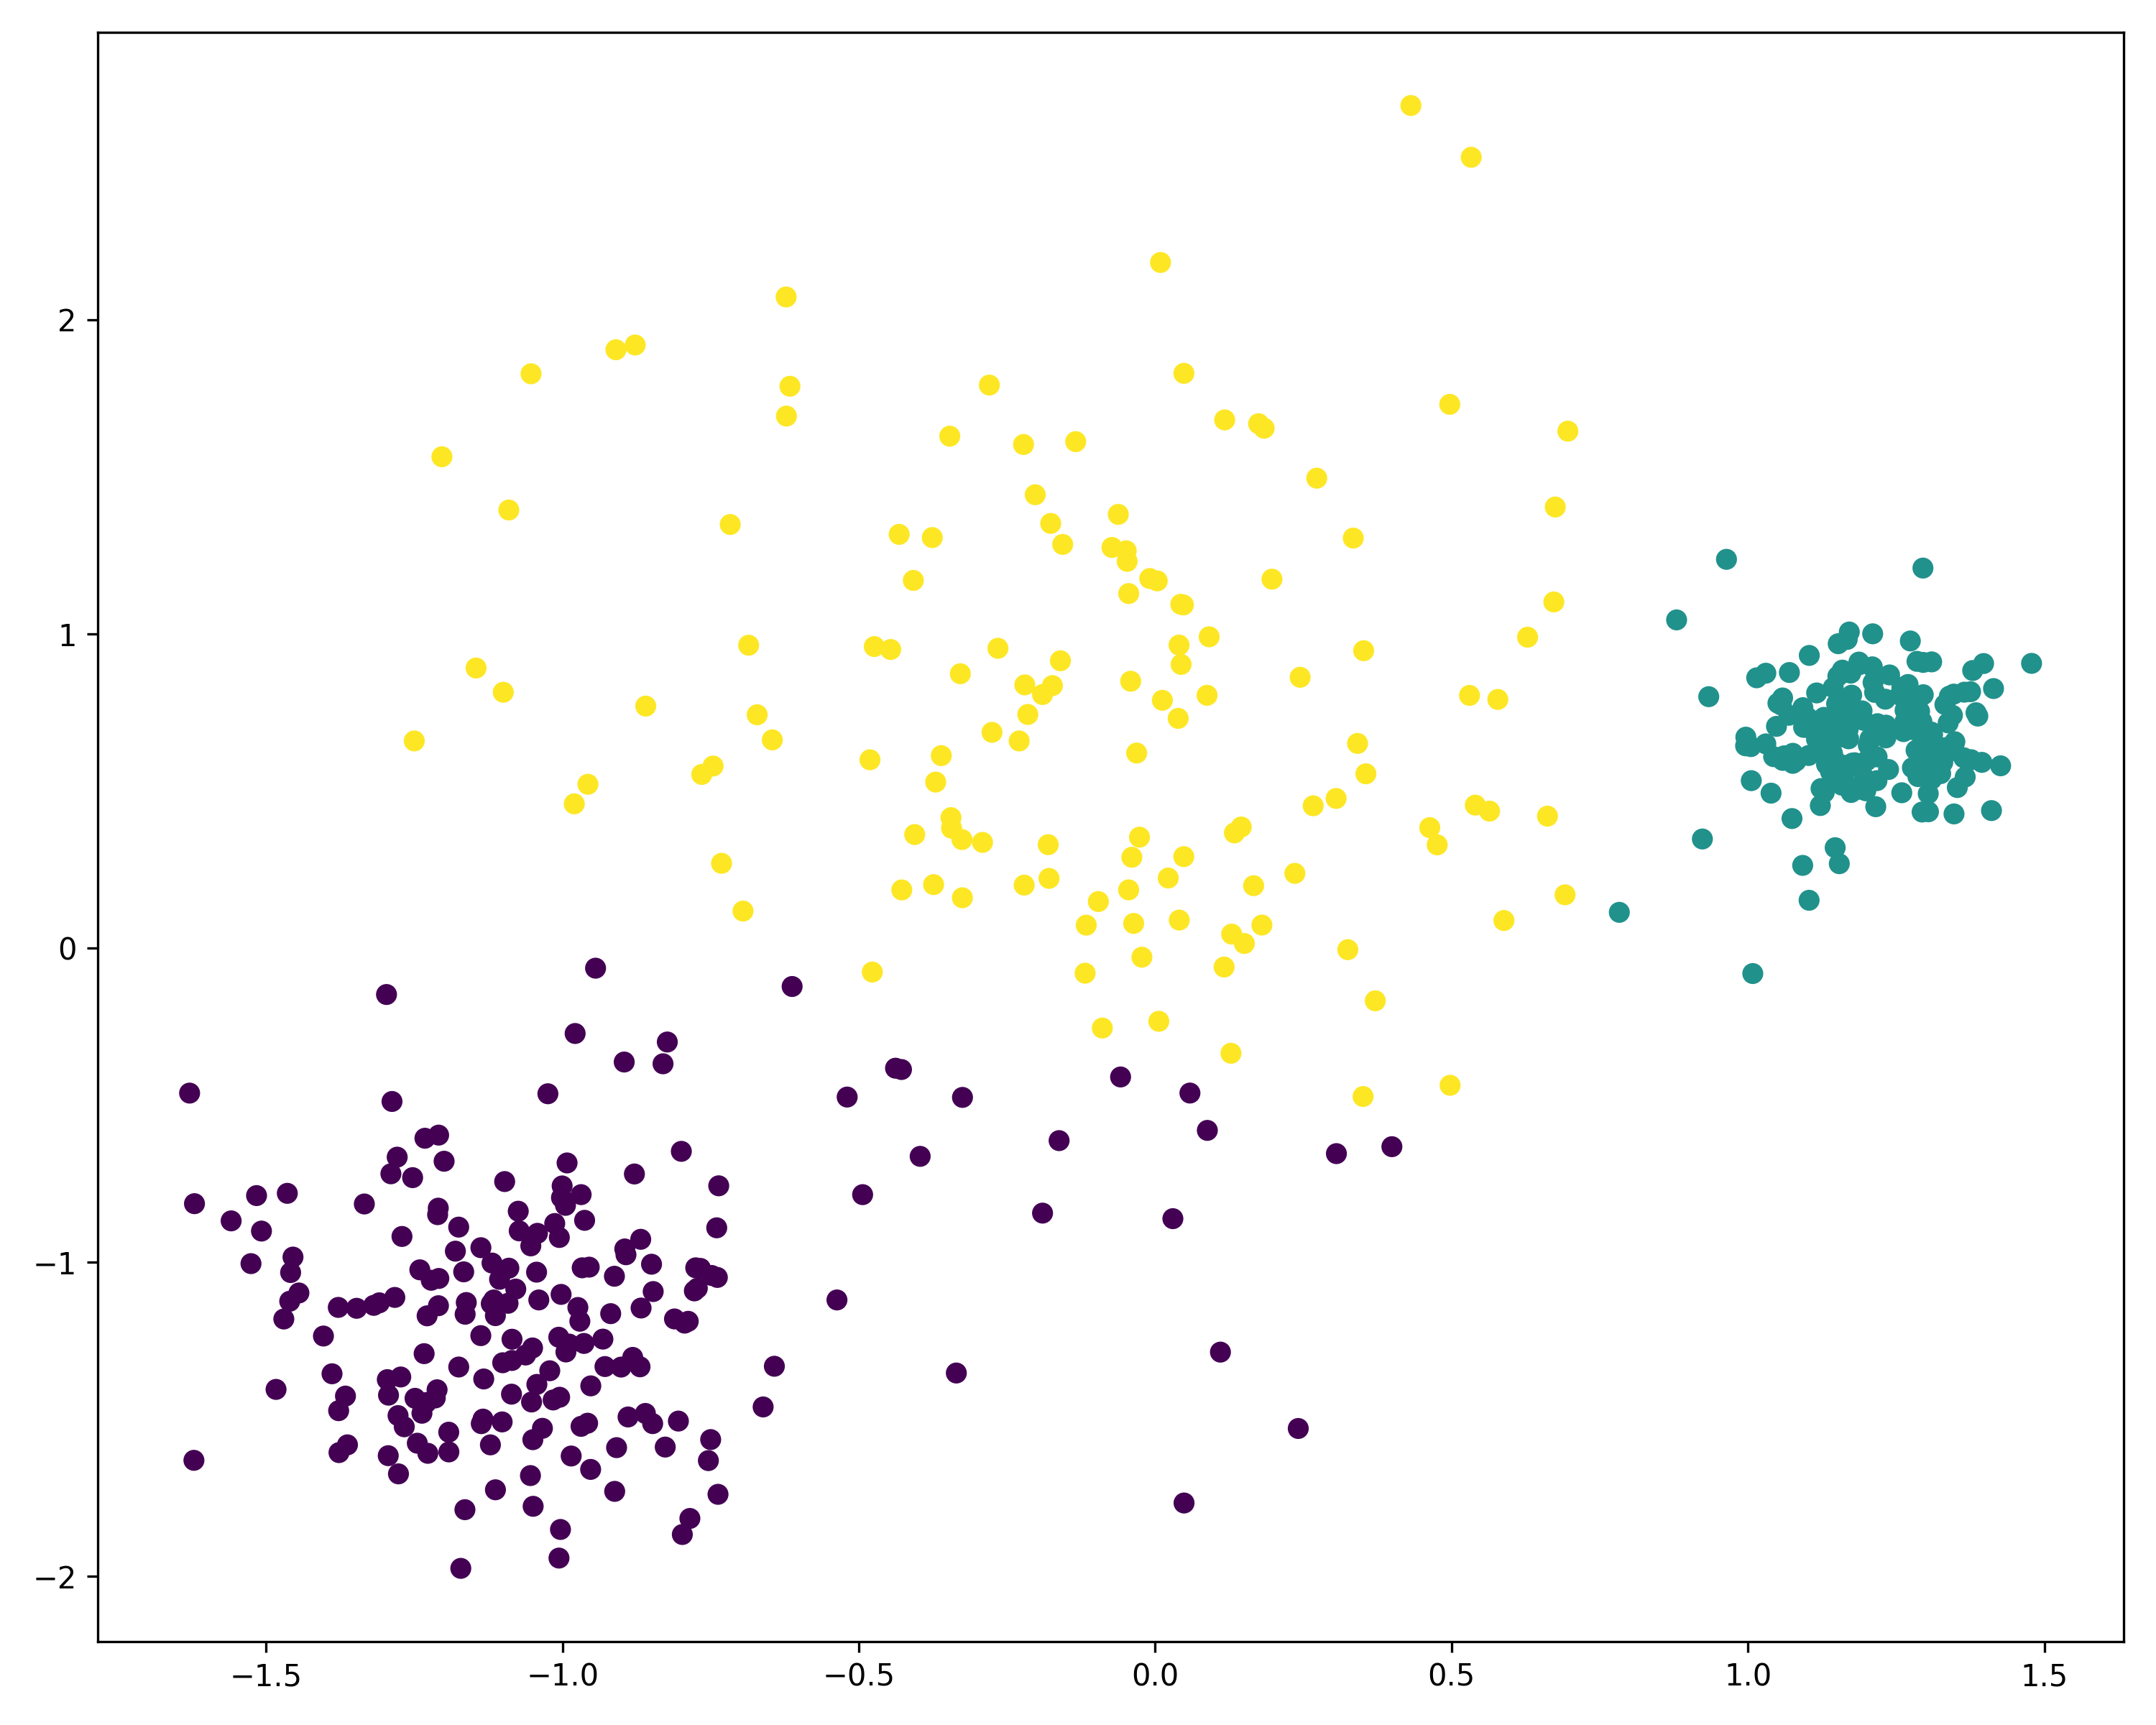
\includegraphics[width=\linewidth]{images/claire/random_n0_varied_spectral_clustering_n_clusters_3_eigen_solver_arpack_affinity_nearest_neighbors.png}
\end{minipage}
\caption{Partições de K-means, Kernel K-means e Spectral Clustering ($K = 3$) empatadas na segunda posição para o conjunto Varied.}
\end{figure}

\begin{figure}
\centering
\begin{minipage}{.23\textwidth}
  \centering
  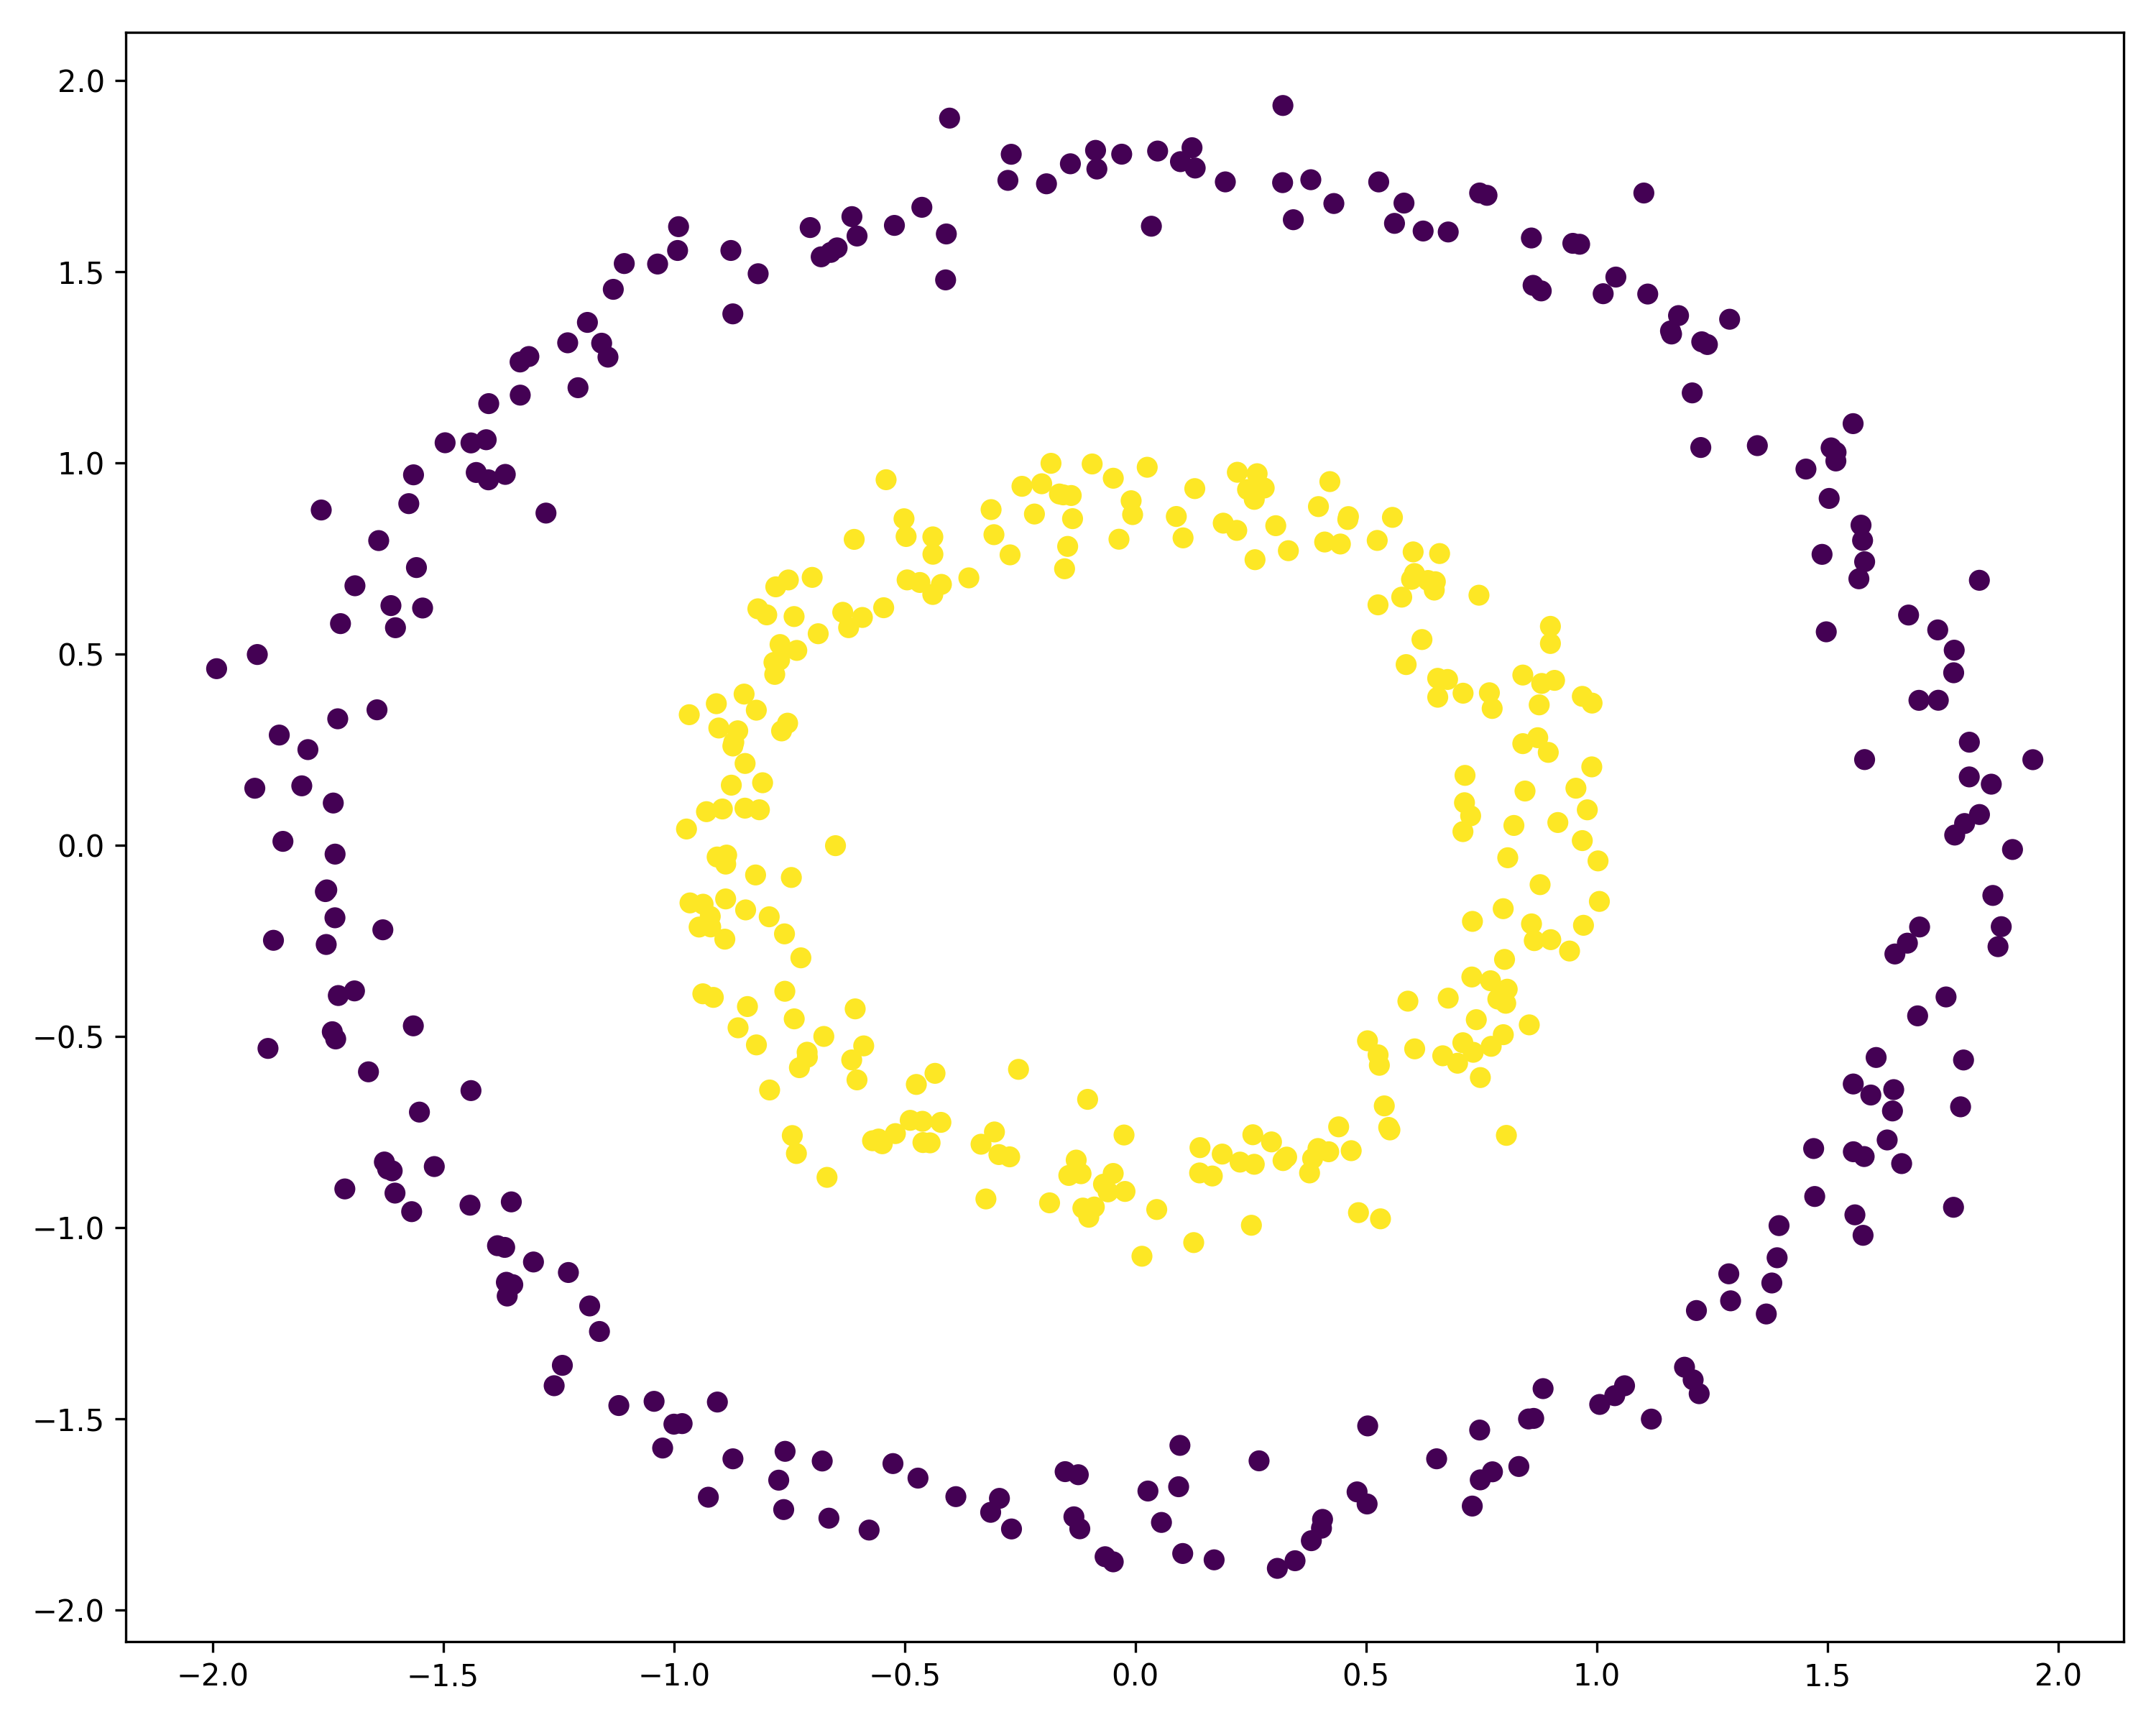
\includegraphics[width=\linewidth]{images/claire/random_n0_noisy_circles_optics_min_samples_7_xi_0_08_min_cluster_size_0_1.png}
\end{minipage}%
\hspace{0.02cm}
\begin{minipage}{.23\textwidth}
  \centering
  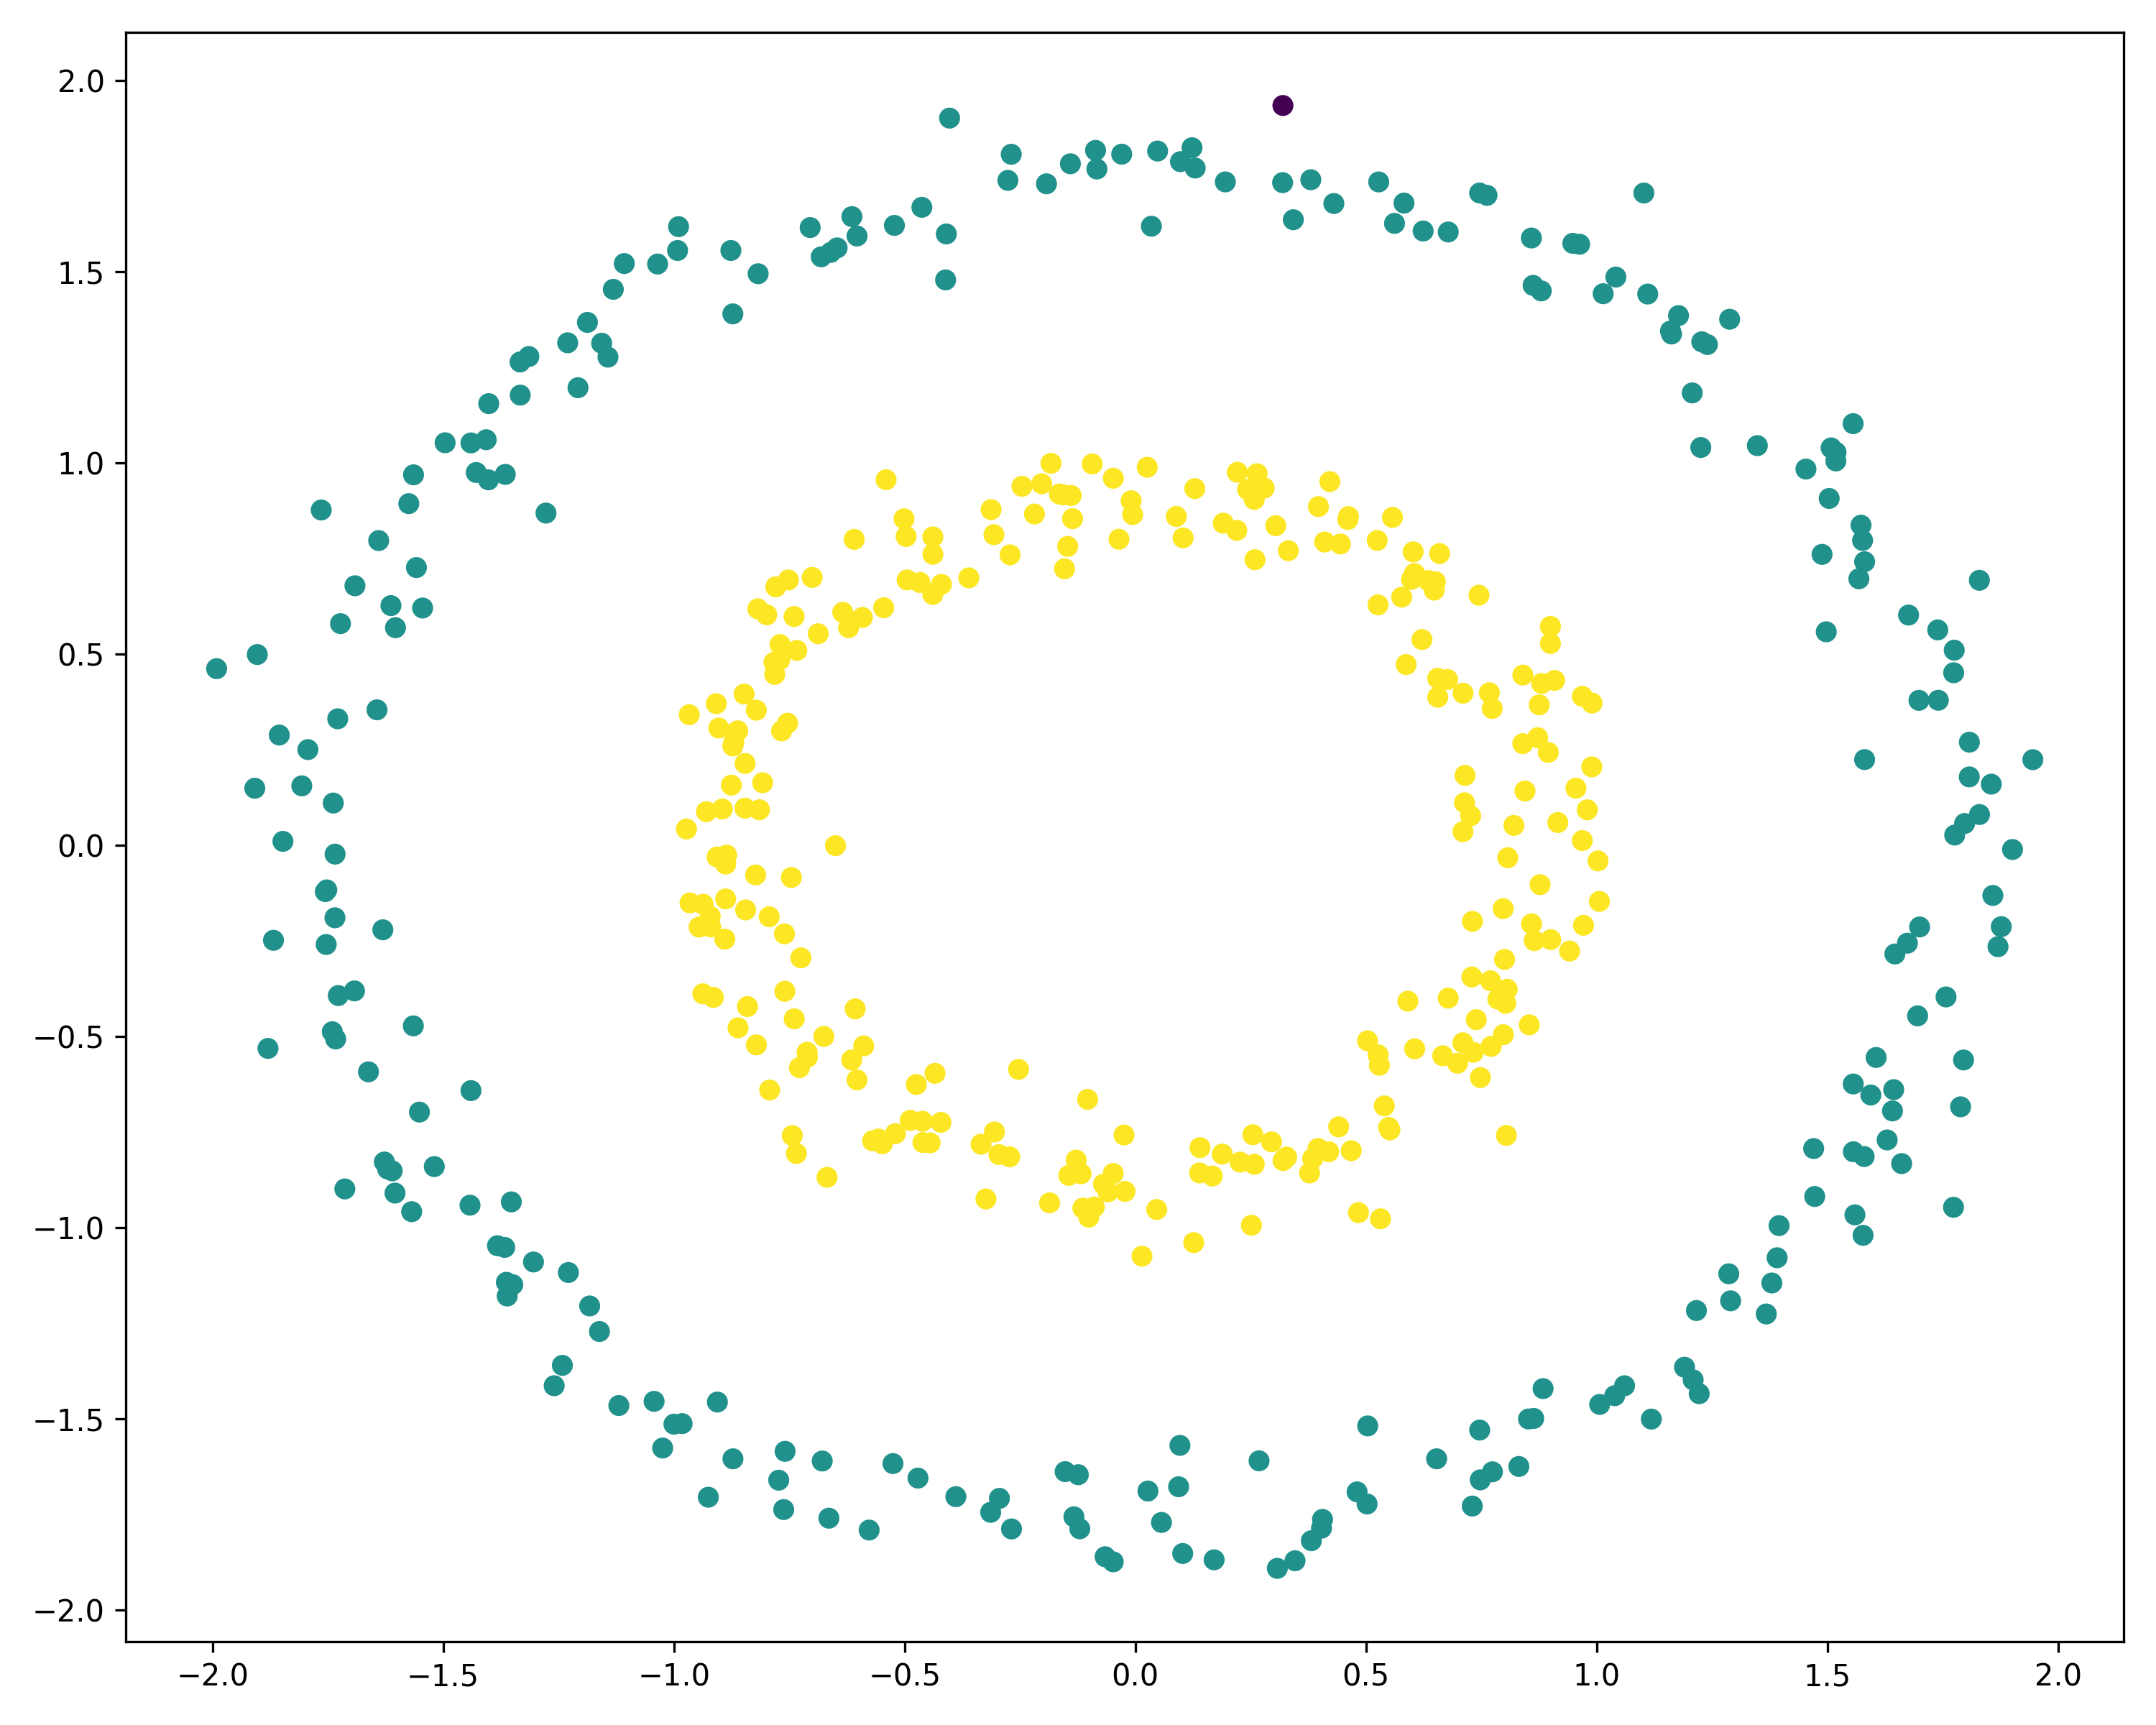
\includegraphics[width=\linewidth]{images/claire/random_n0_noisy_circles_dbscan_eps_0_2_min_samples_2.png}
\end{minipage}
\vspace{0.02cm}
\begin{minipage}{.23\textwidth}
  \centering
  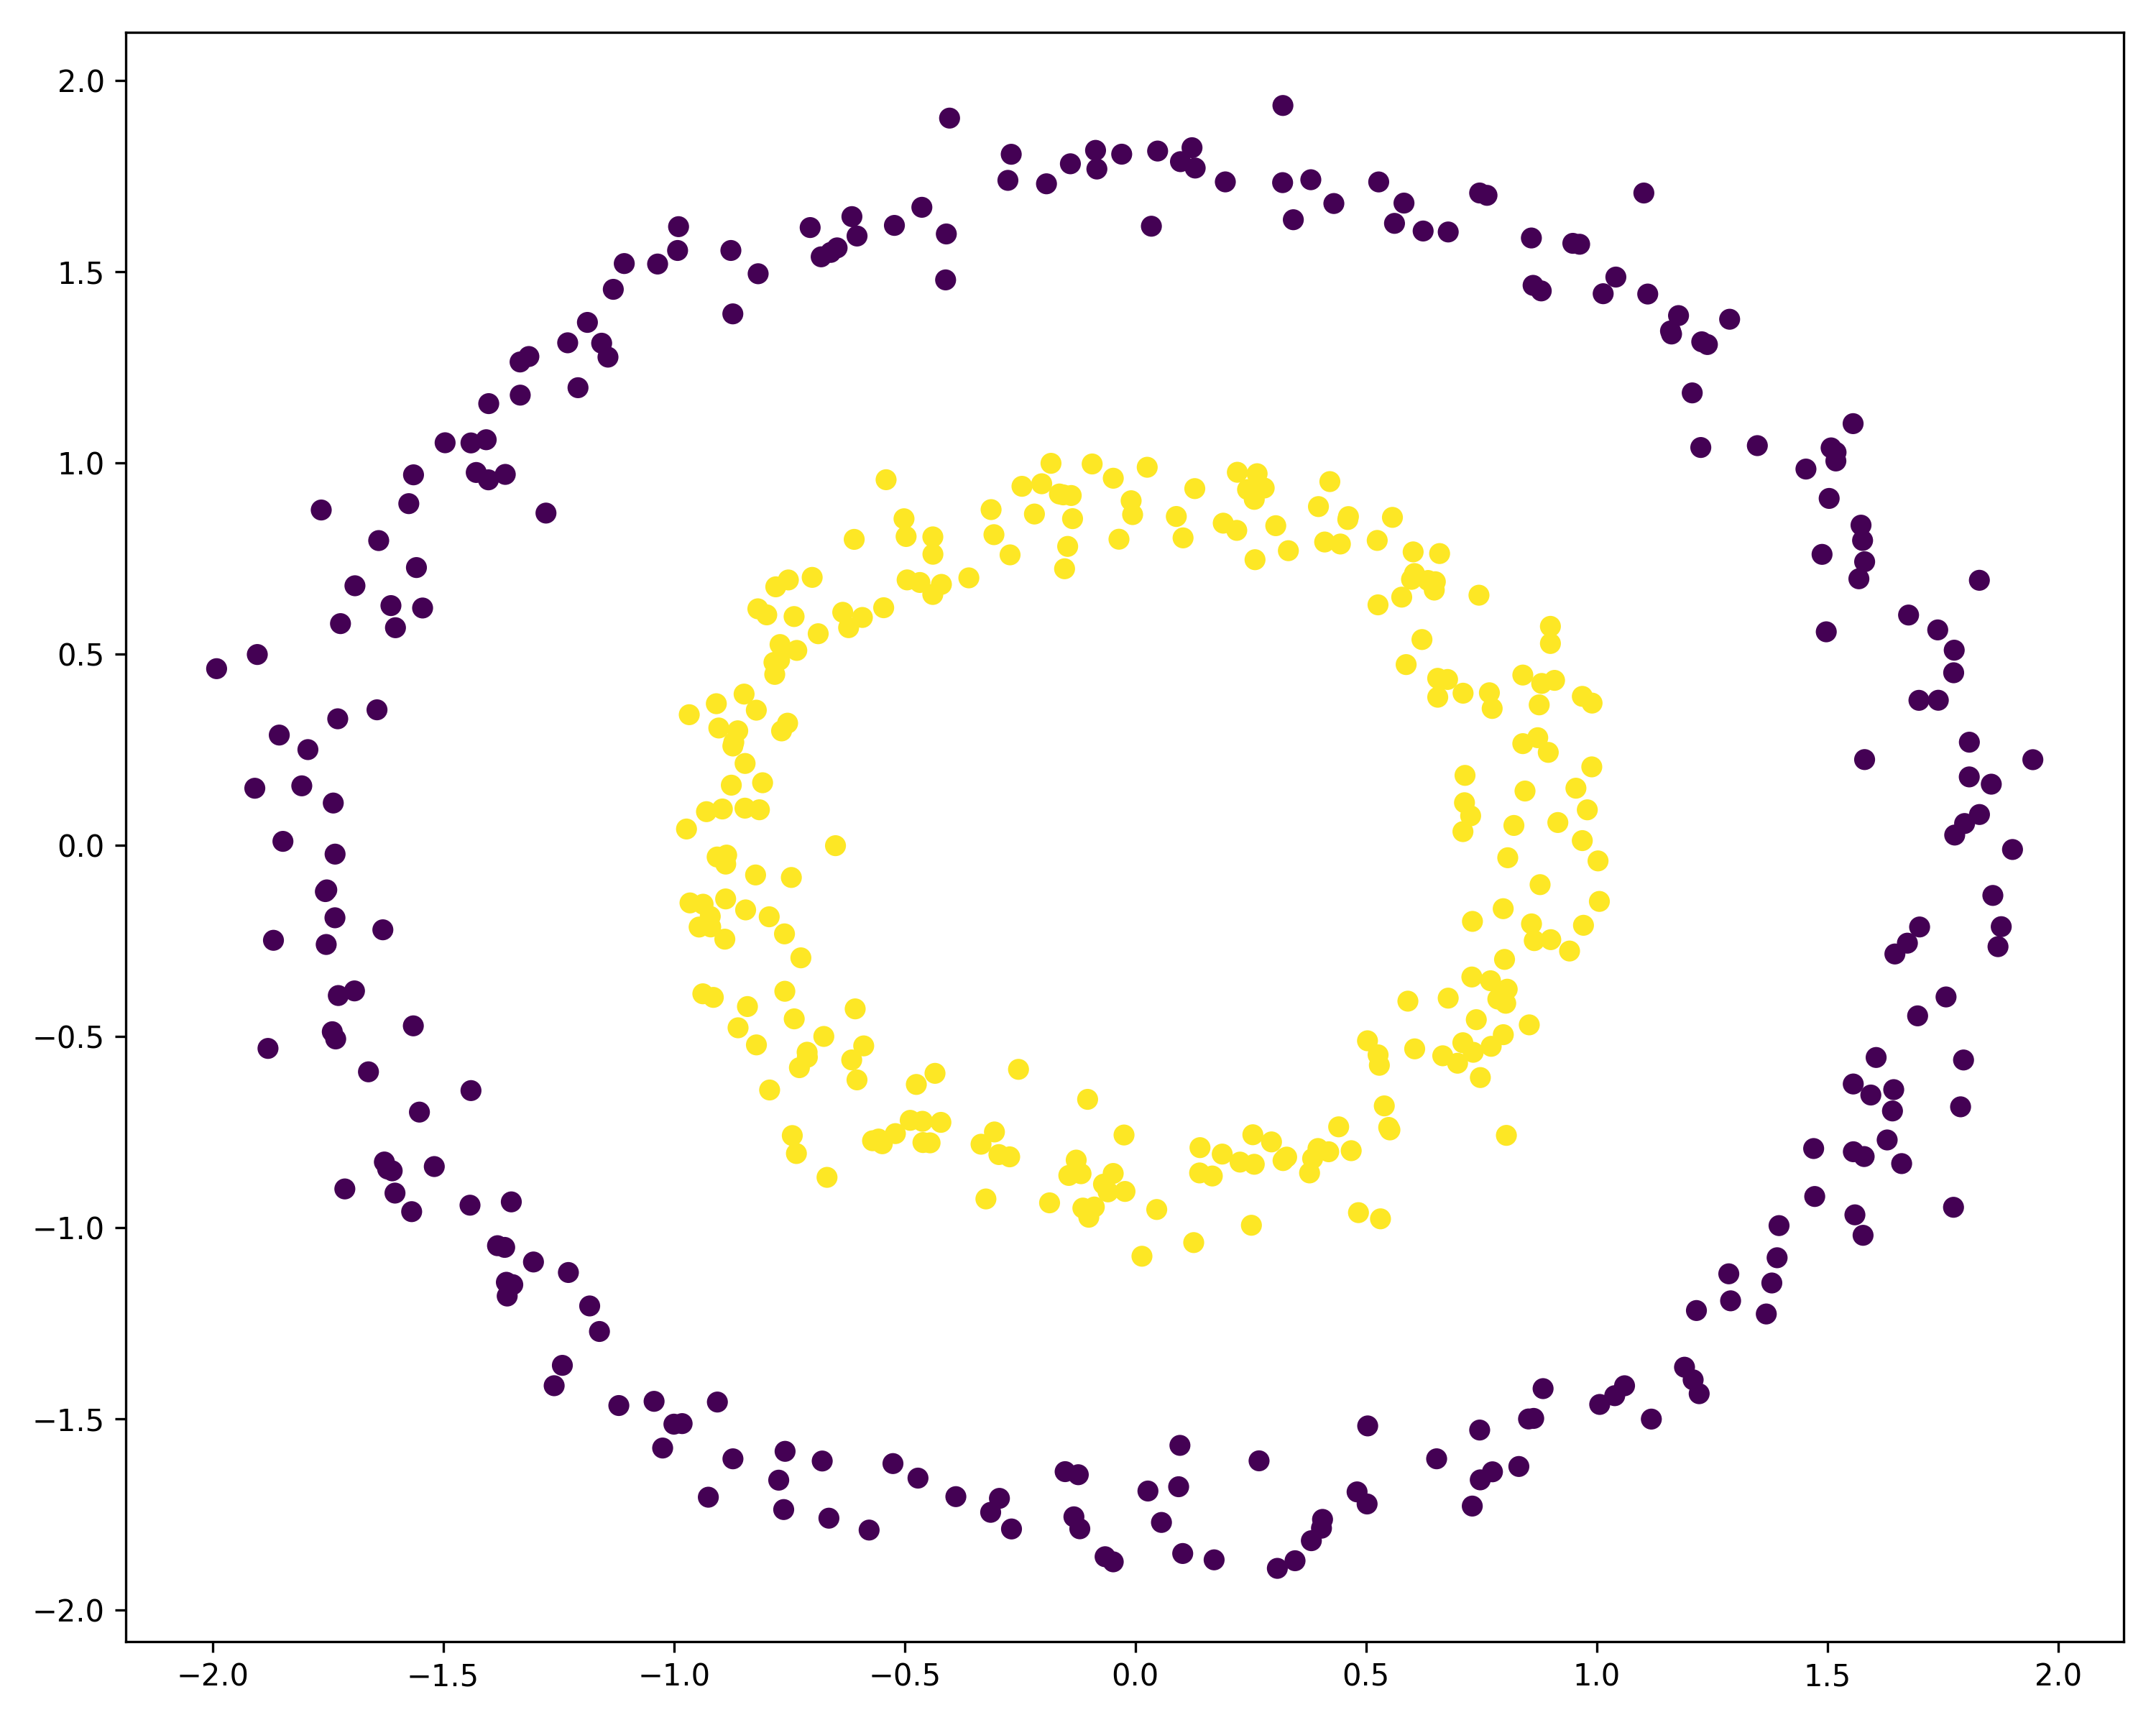
\includegraphics[width=\linewidth]{images/claire/random_n0_noisy_circles_dbscan_eps_0_3_min_samples_2.png}
\end{minipage}
\hspace{0.02cm}
\begin{minipage}{.23\textwidth}
  \centering
  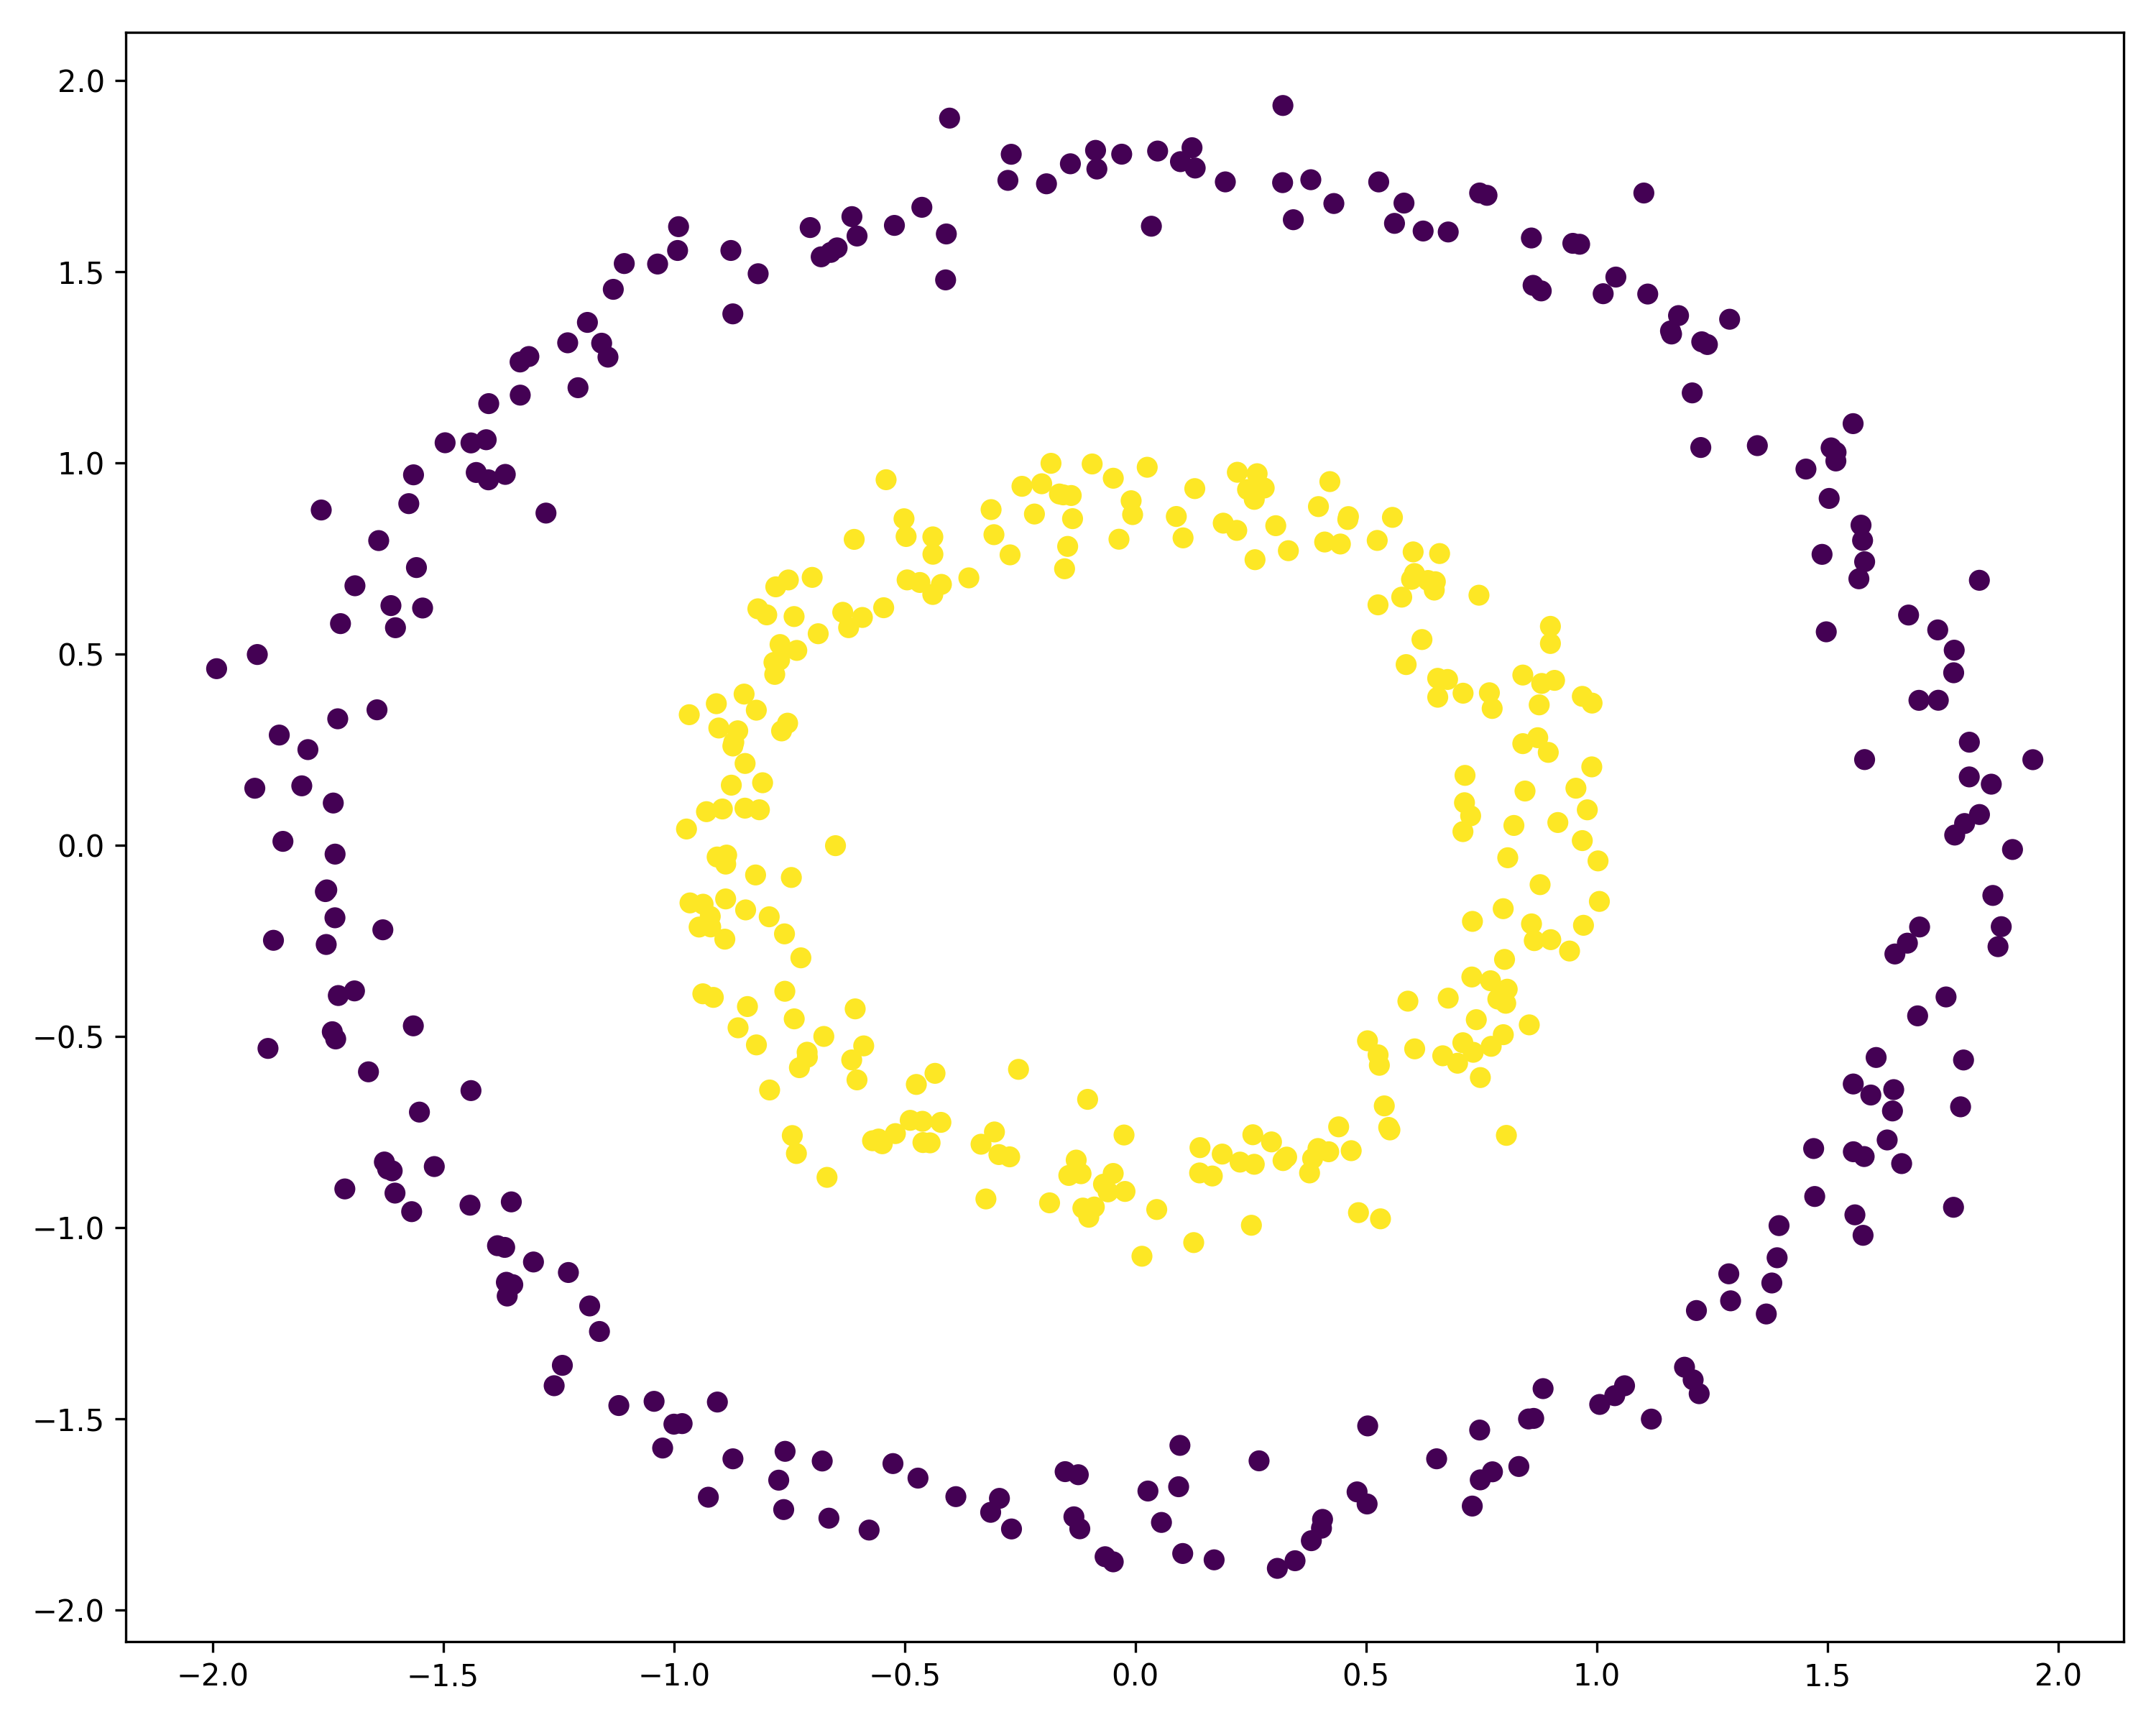
\includegraphics[width=\linewidth]{images/claire/random_n0_noisy_circles_dbscan_eps_0_4_min_samples_2.png}
\end{minipage}
\vspace{0.02cm}
\begin{minipage}{.23\textwidth}
  \centering
  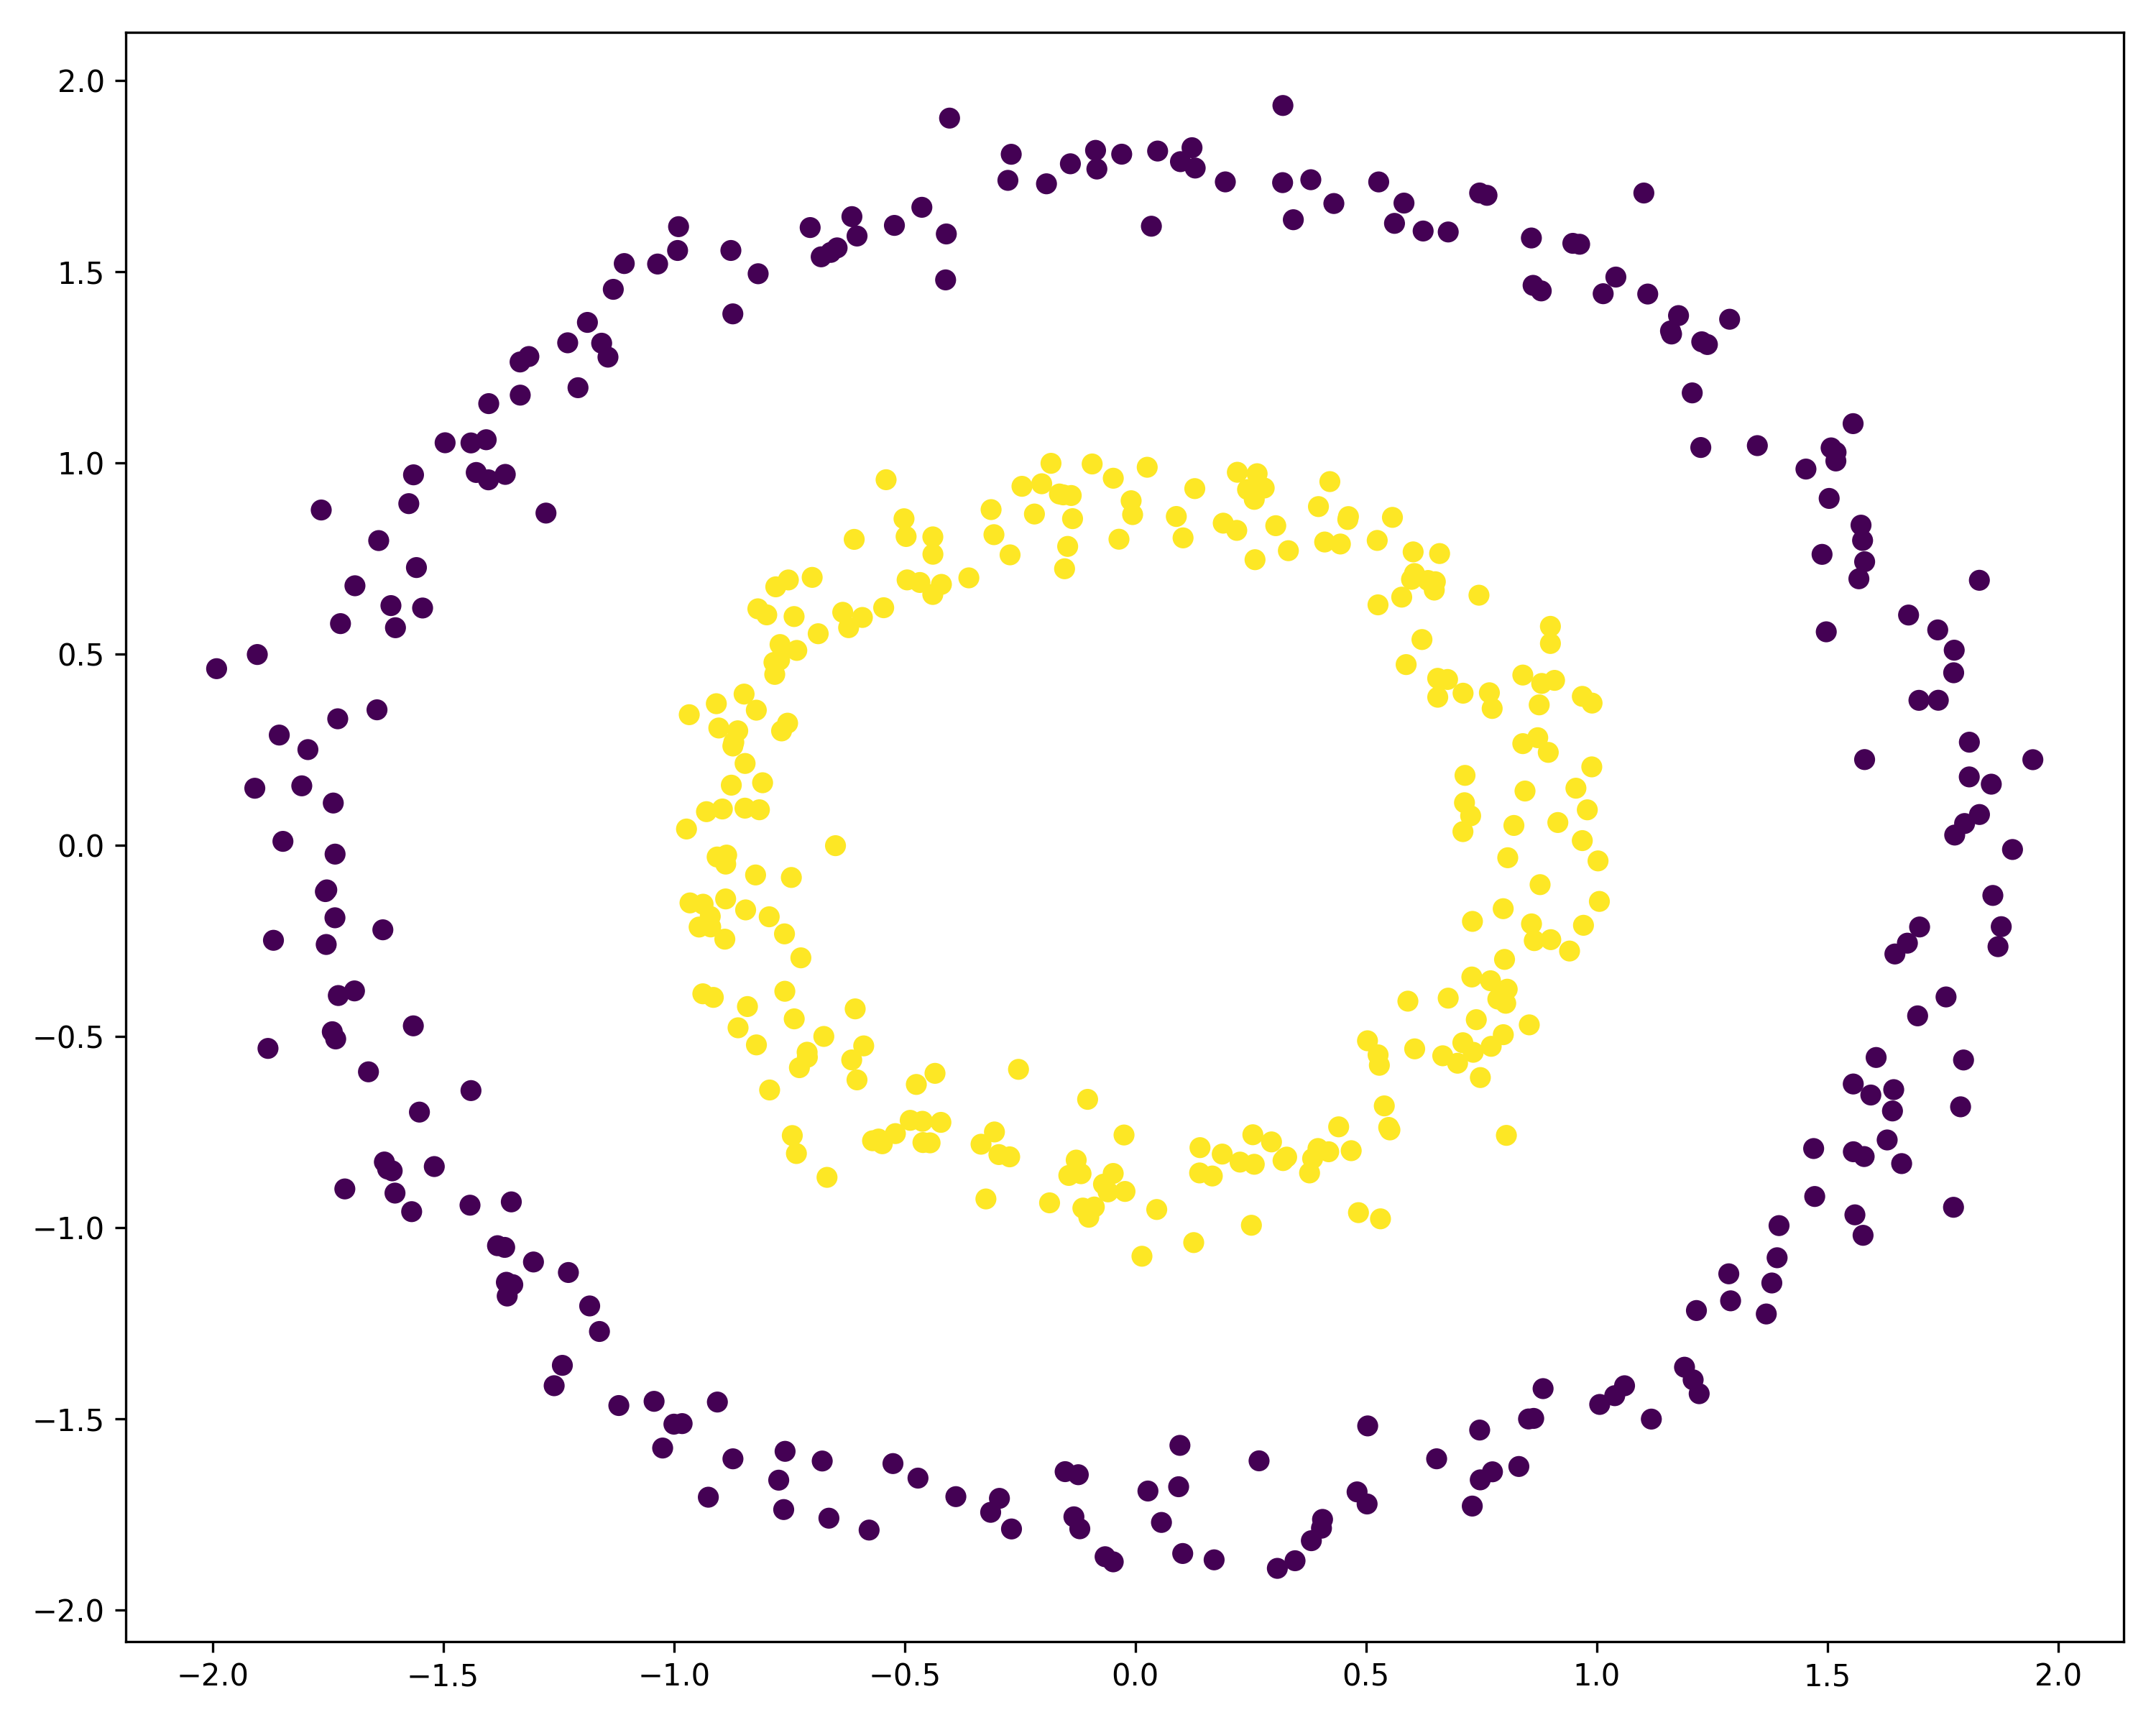
\includegraphics[width=\linewidth]{images/claire/random_n0_noisy_circles_dbscan_eps_0_5_min_samples_2.png}
\end{minipage}
\hspace{0.02cm}
\begin{minipage}{.23\textwidth}
  \centering
  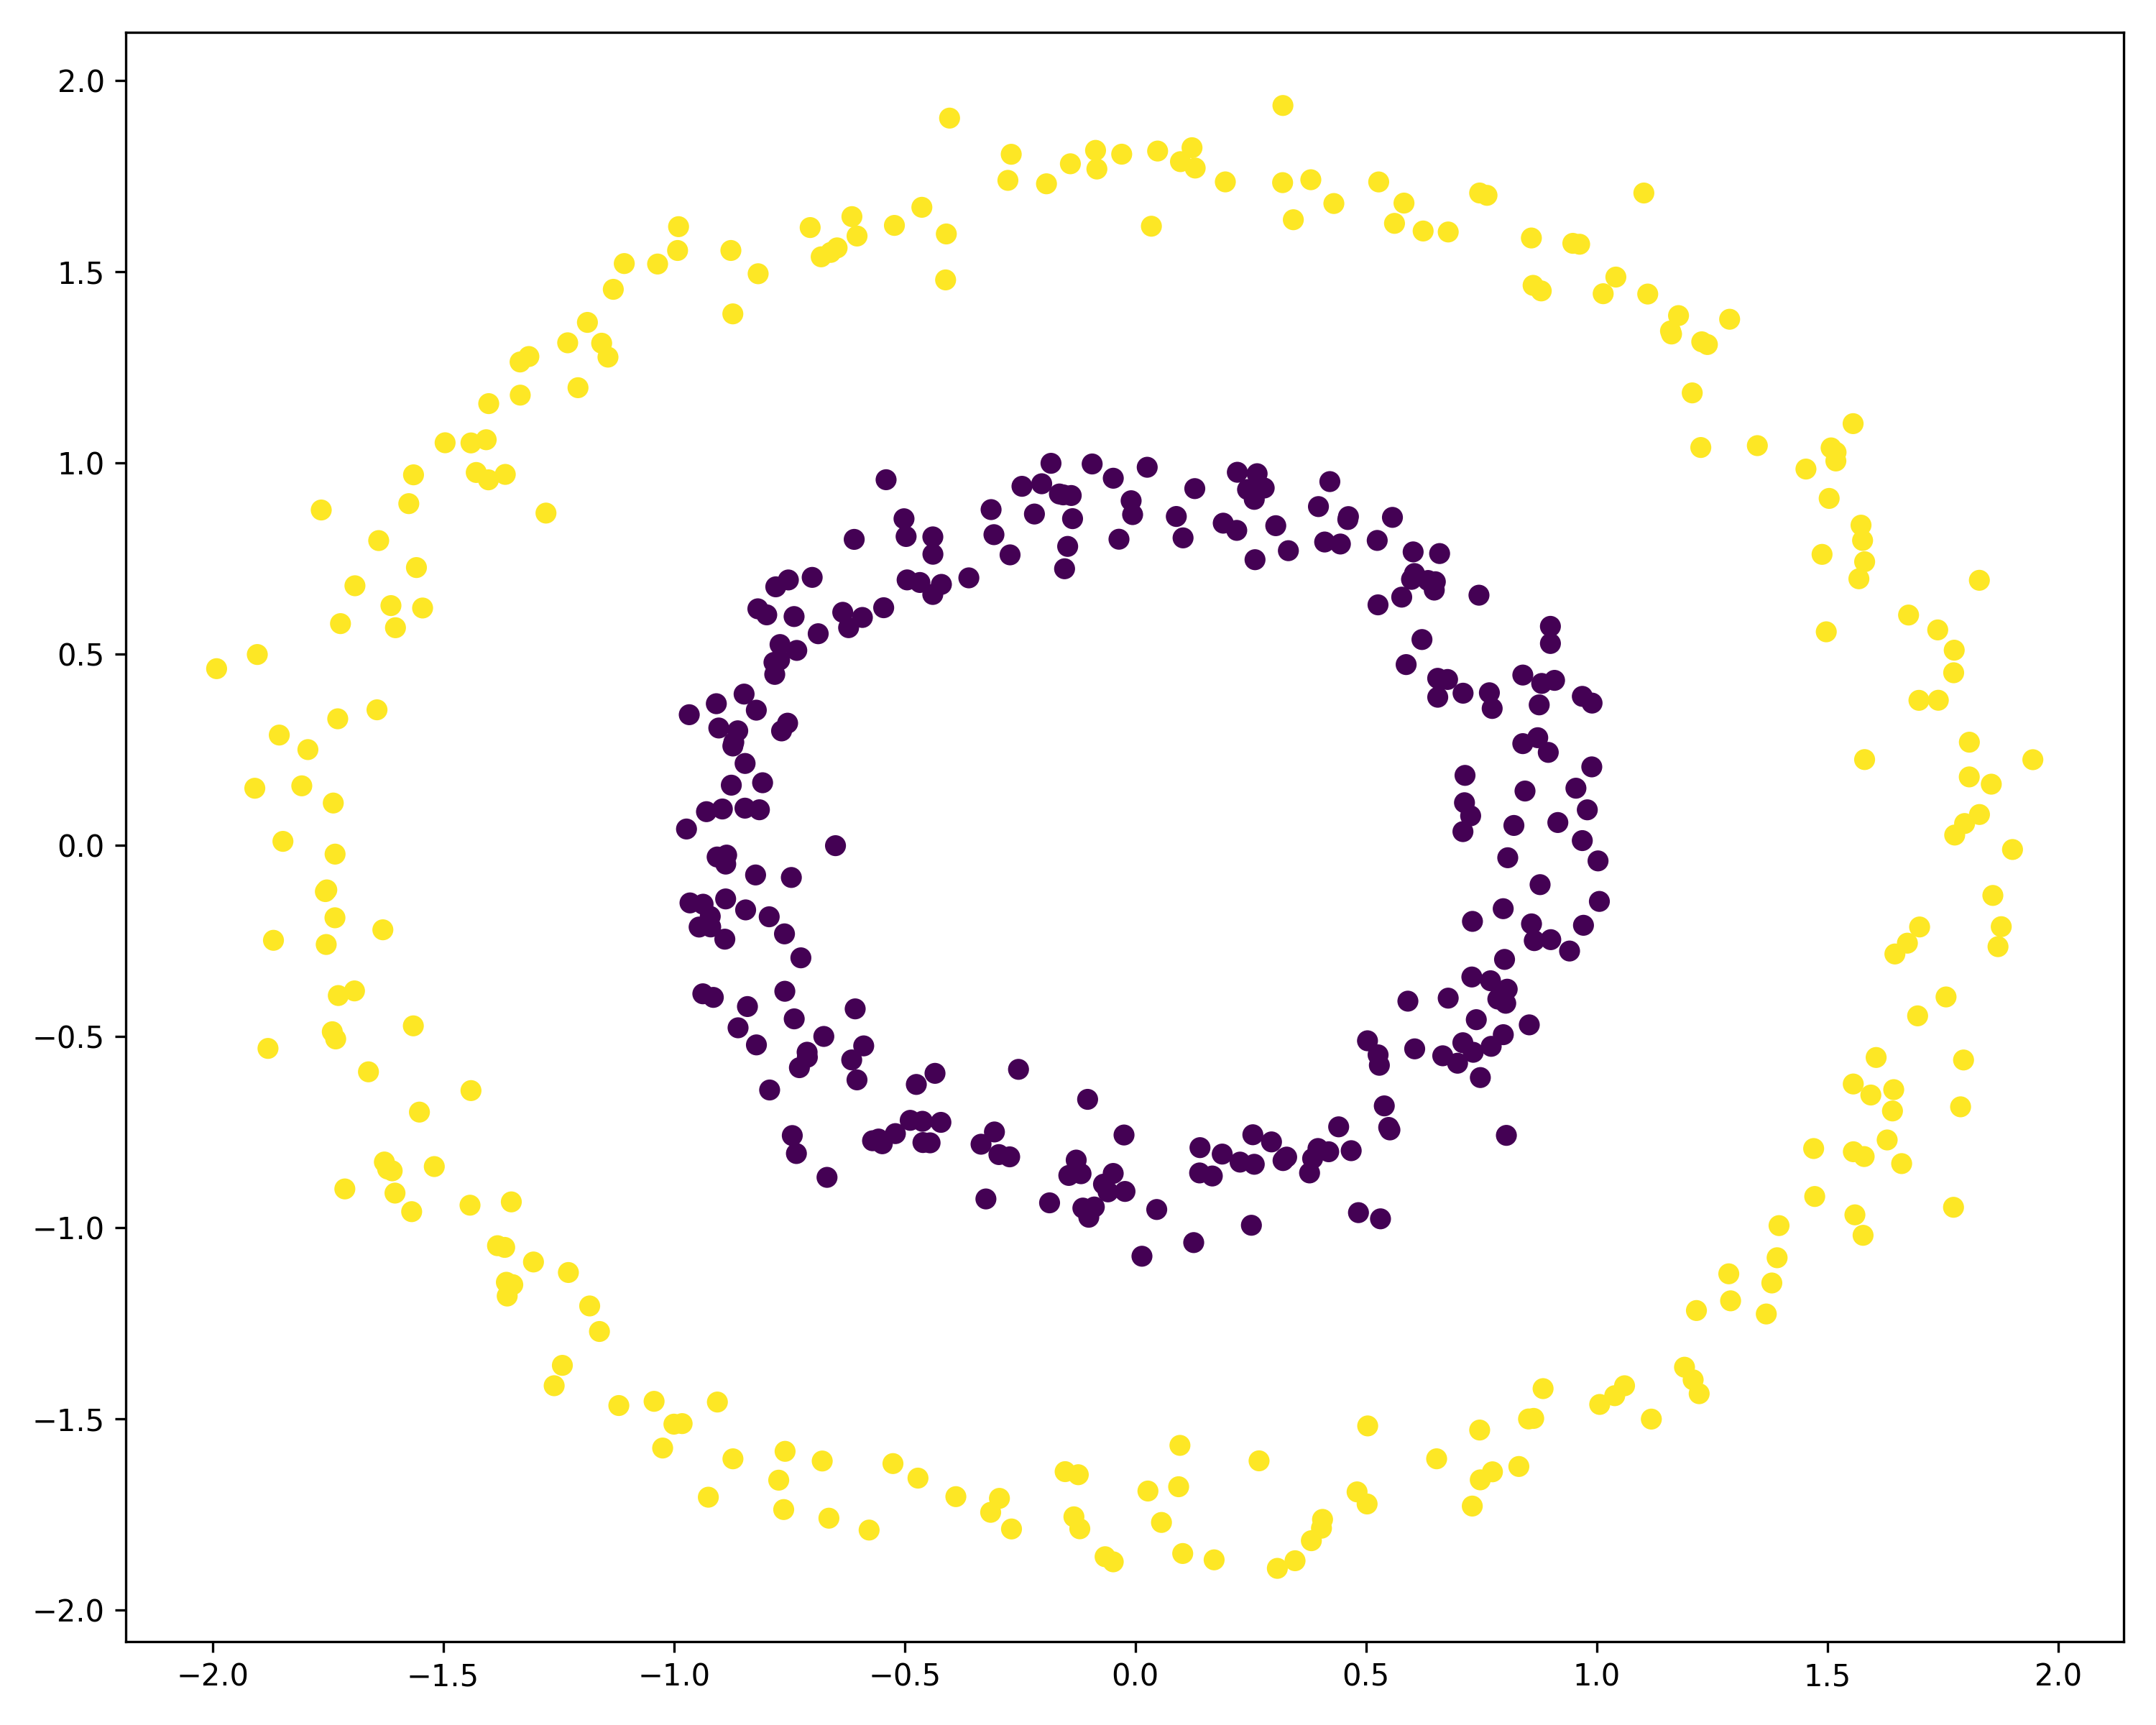
\includegraphics[width=\linewidth]{images/claire/random_n0_noisy_circles_spectral_clustering_n_clusters_2_eigen_solver_arpack_affinity_nearest_neighbors.png}
\end{minipage}
\vspace{0.02cm}
\begin{minipage}{.23\textwidth}
  \centering
  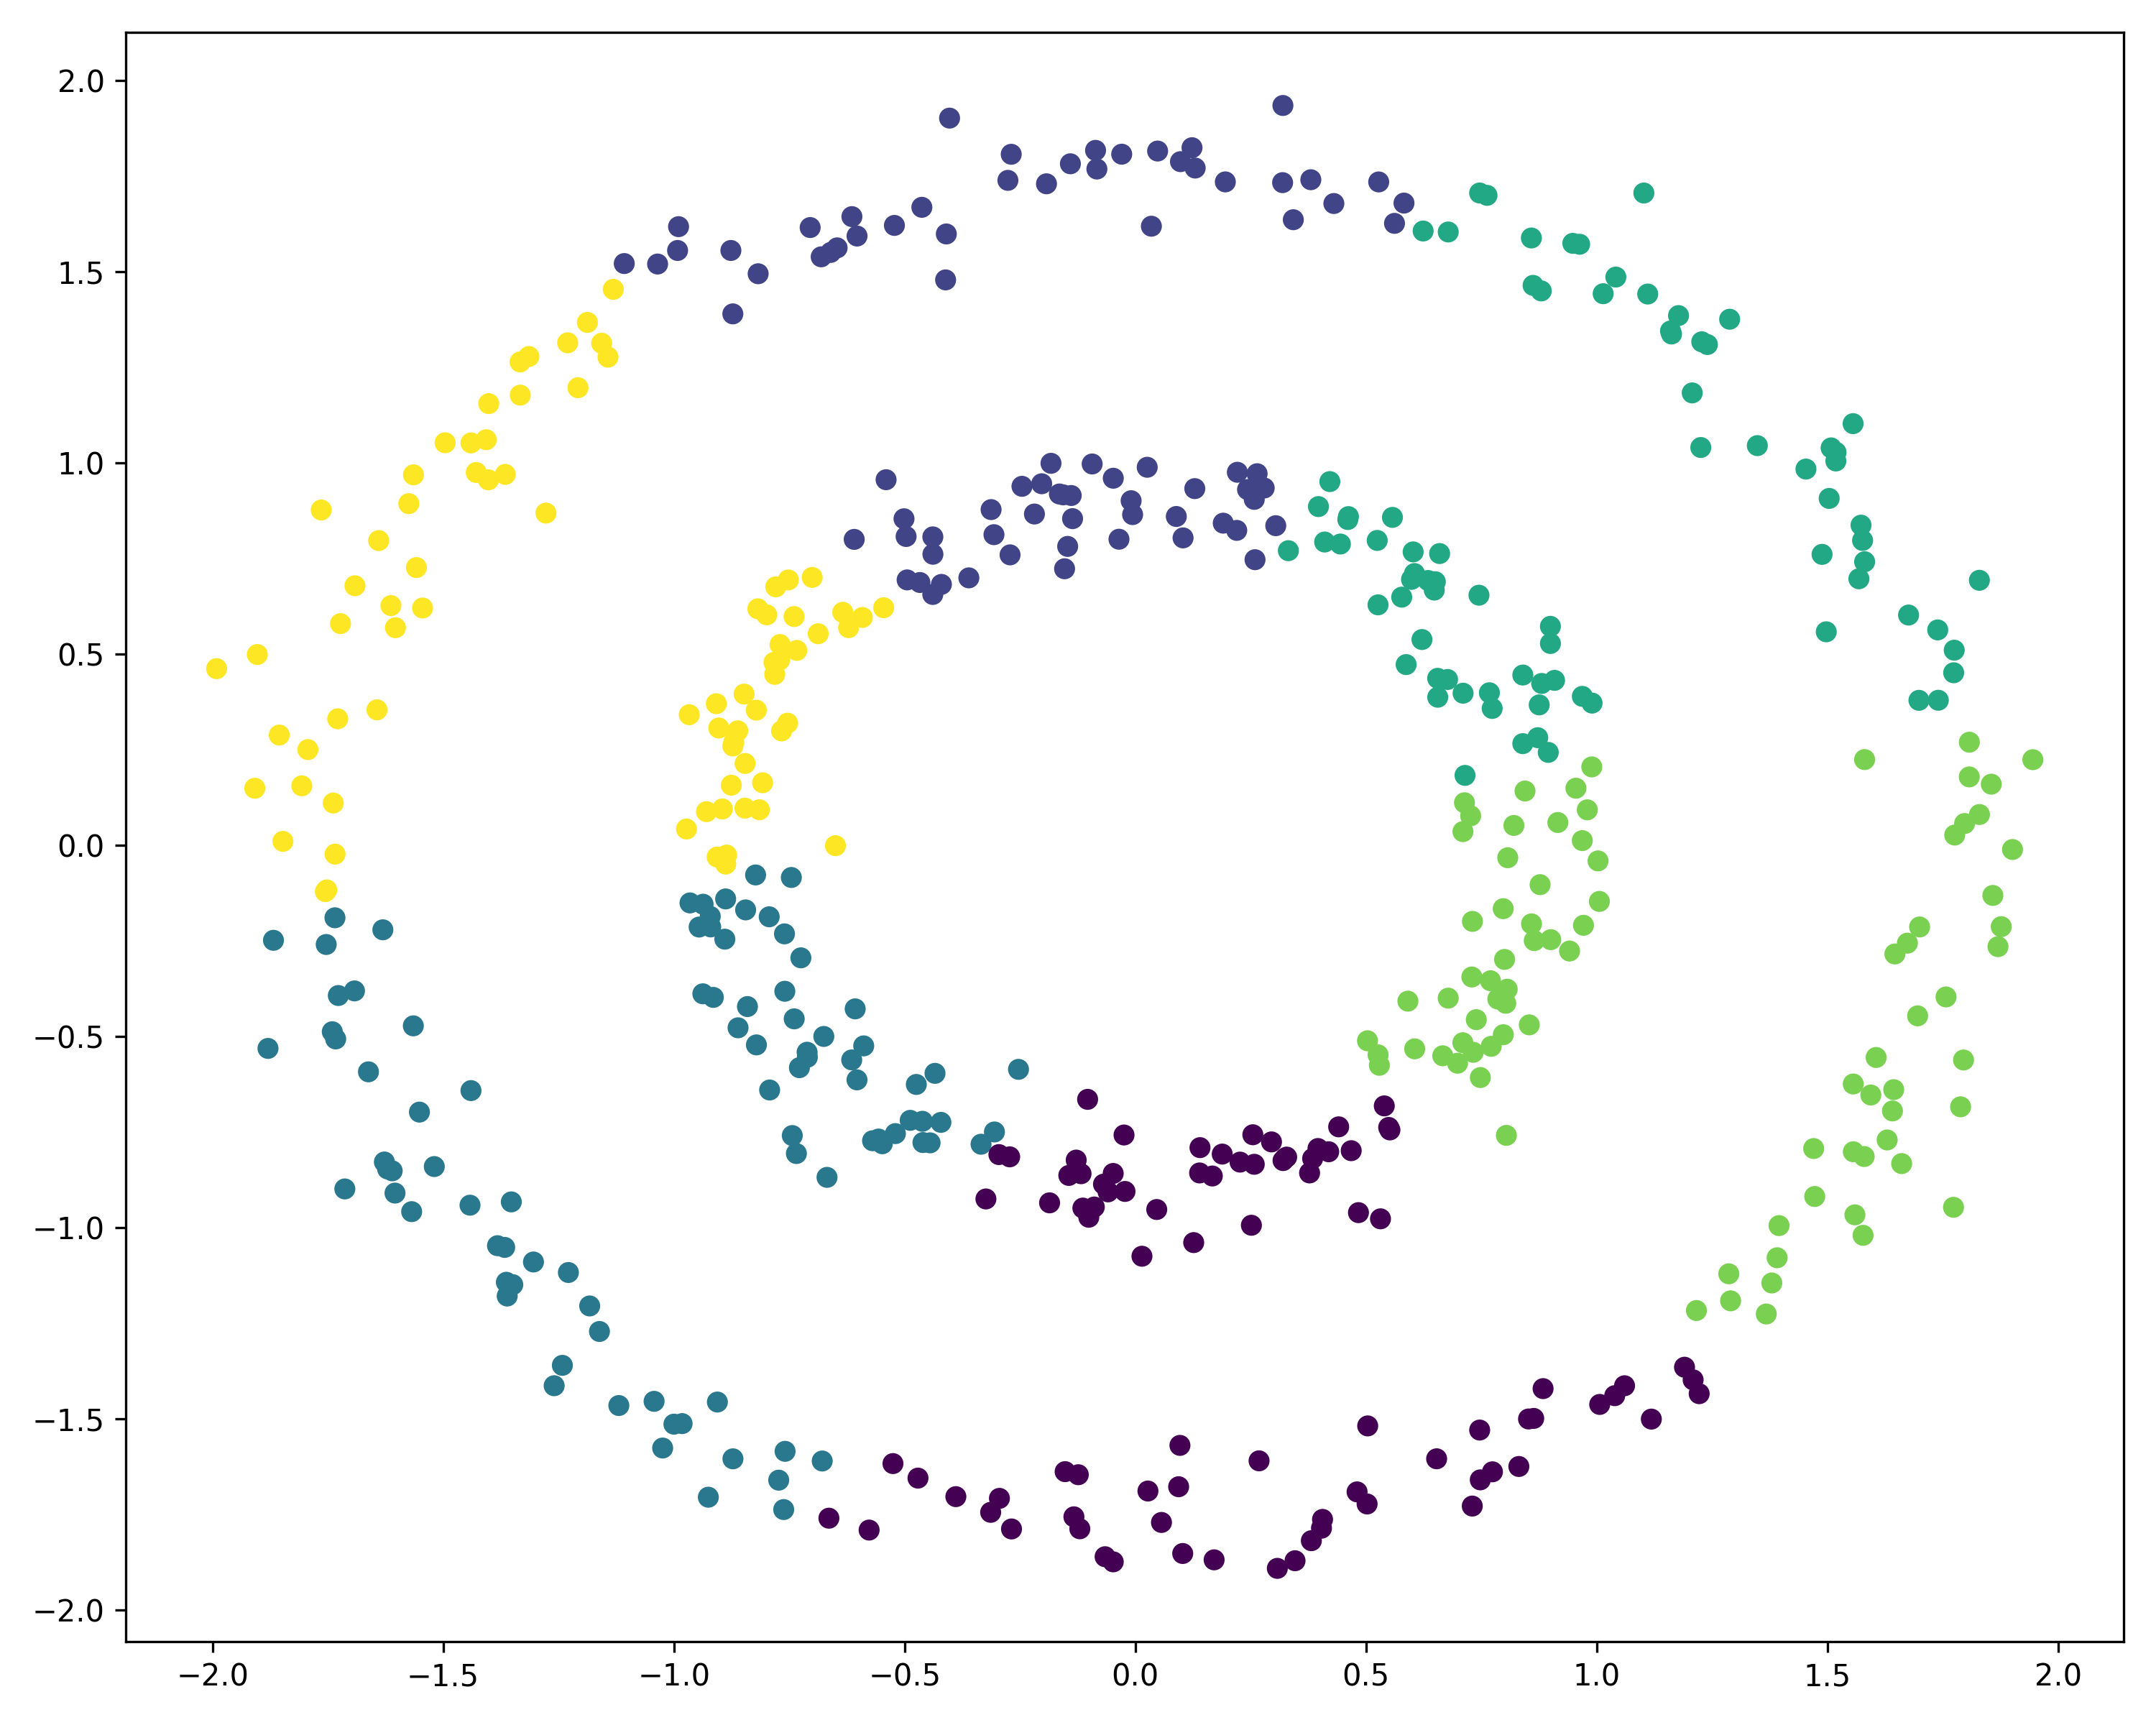
\includegraphics[width=\linewidth]{images/claire/random_n0_noisy_circles_kmeans_n_clusters_6.png}
\end{minipage}
\hspace{0.02cm}
\begin{minipage}{.23\textwidth}
  \centering
  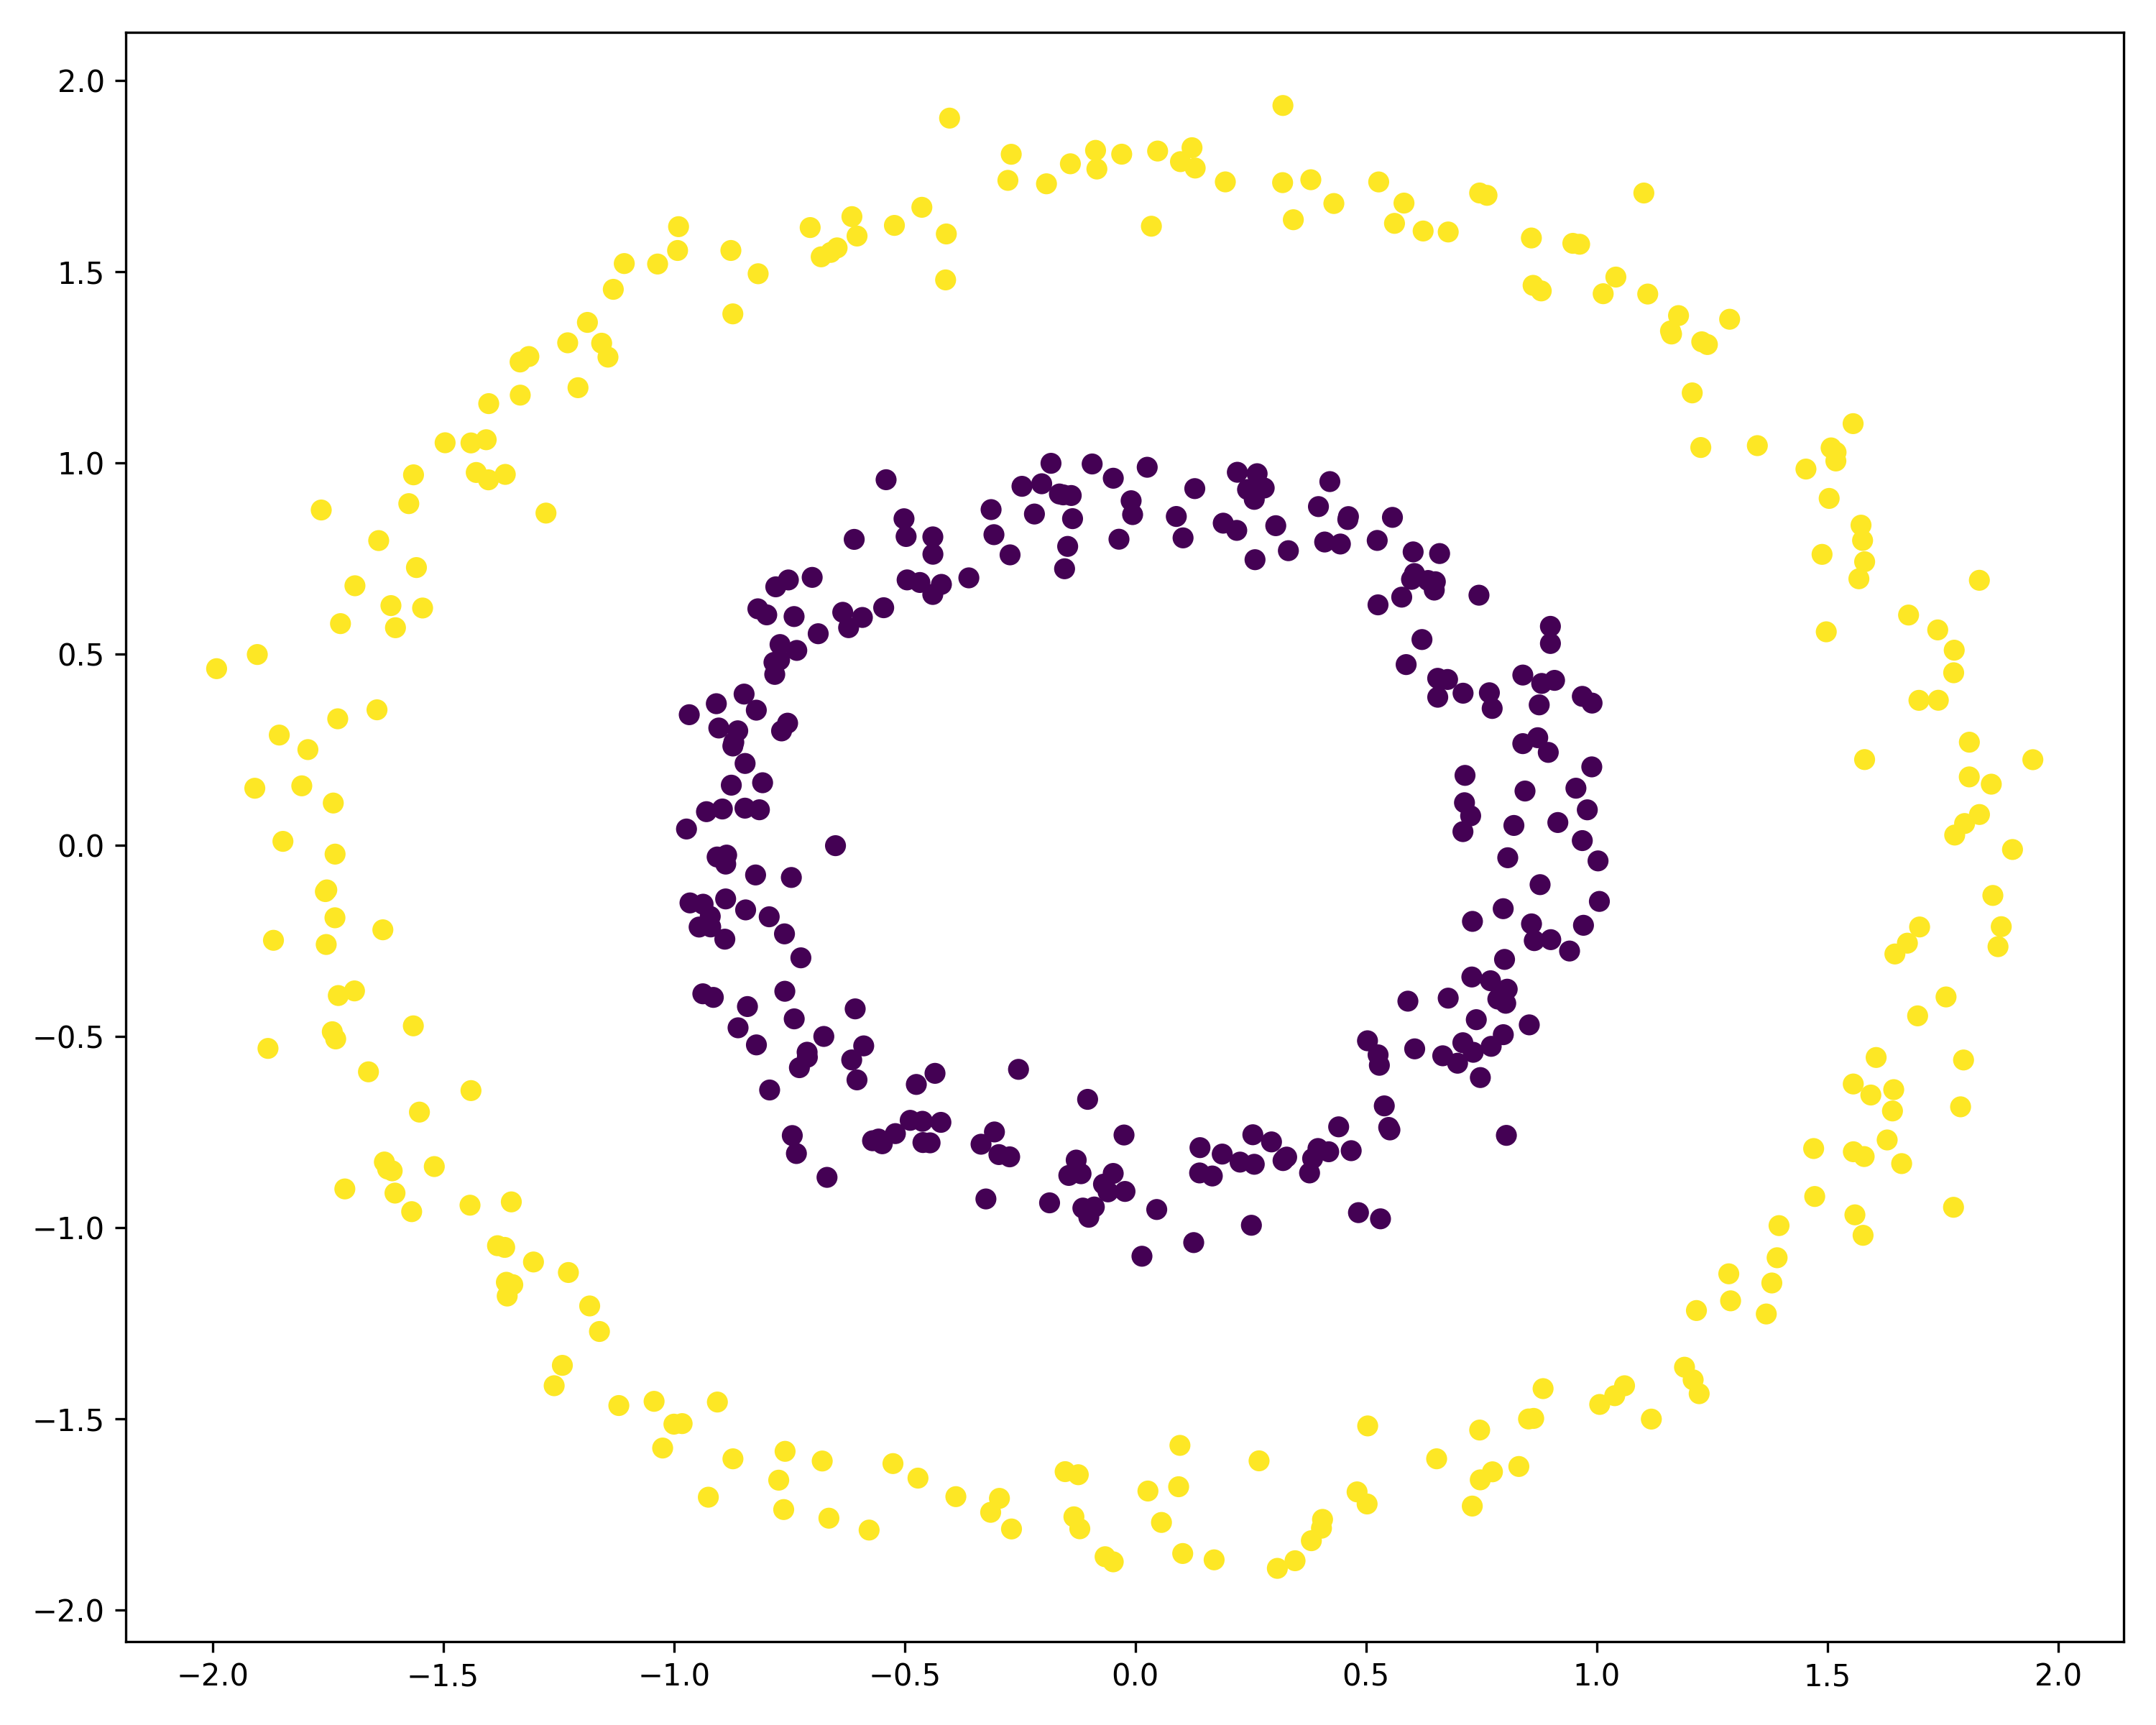
\includegraphics[width=\linewidth]{images/claire/random_n0_noisy_circles_spectral_clustering_n_clusters_2_eigen_solver_arpack_affinity_nearest_neighbors.png}
\end{minipage}
\caption{Partições do OPTICS, com \textsf{min\_samples} = $7$, \textsf{xi} = $0.08$, \textsf{min\_cluster\_size} = $0.1$, DBSCAN com $\epsilon=\{0.2, 0.3, 0.4, 0.5\}$, K-means com $K = 6$ e Spectral Clustering com $K = 2$.}
\end{figure}


\begin{figure}[t]
\centering
\begin{minipage}{.8\textwidth}
  \centering
  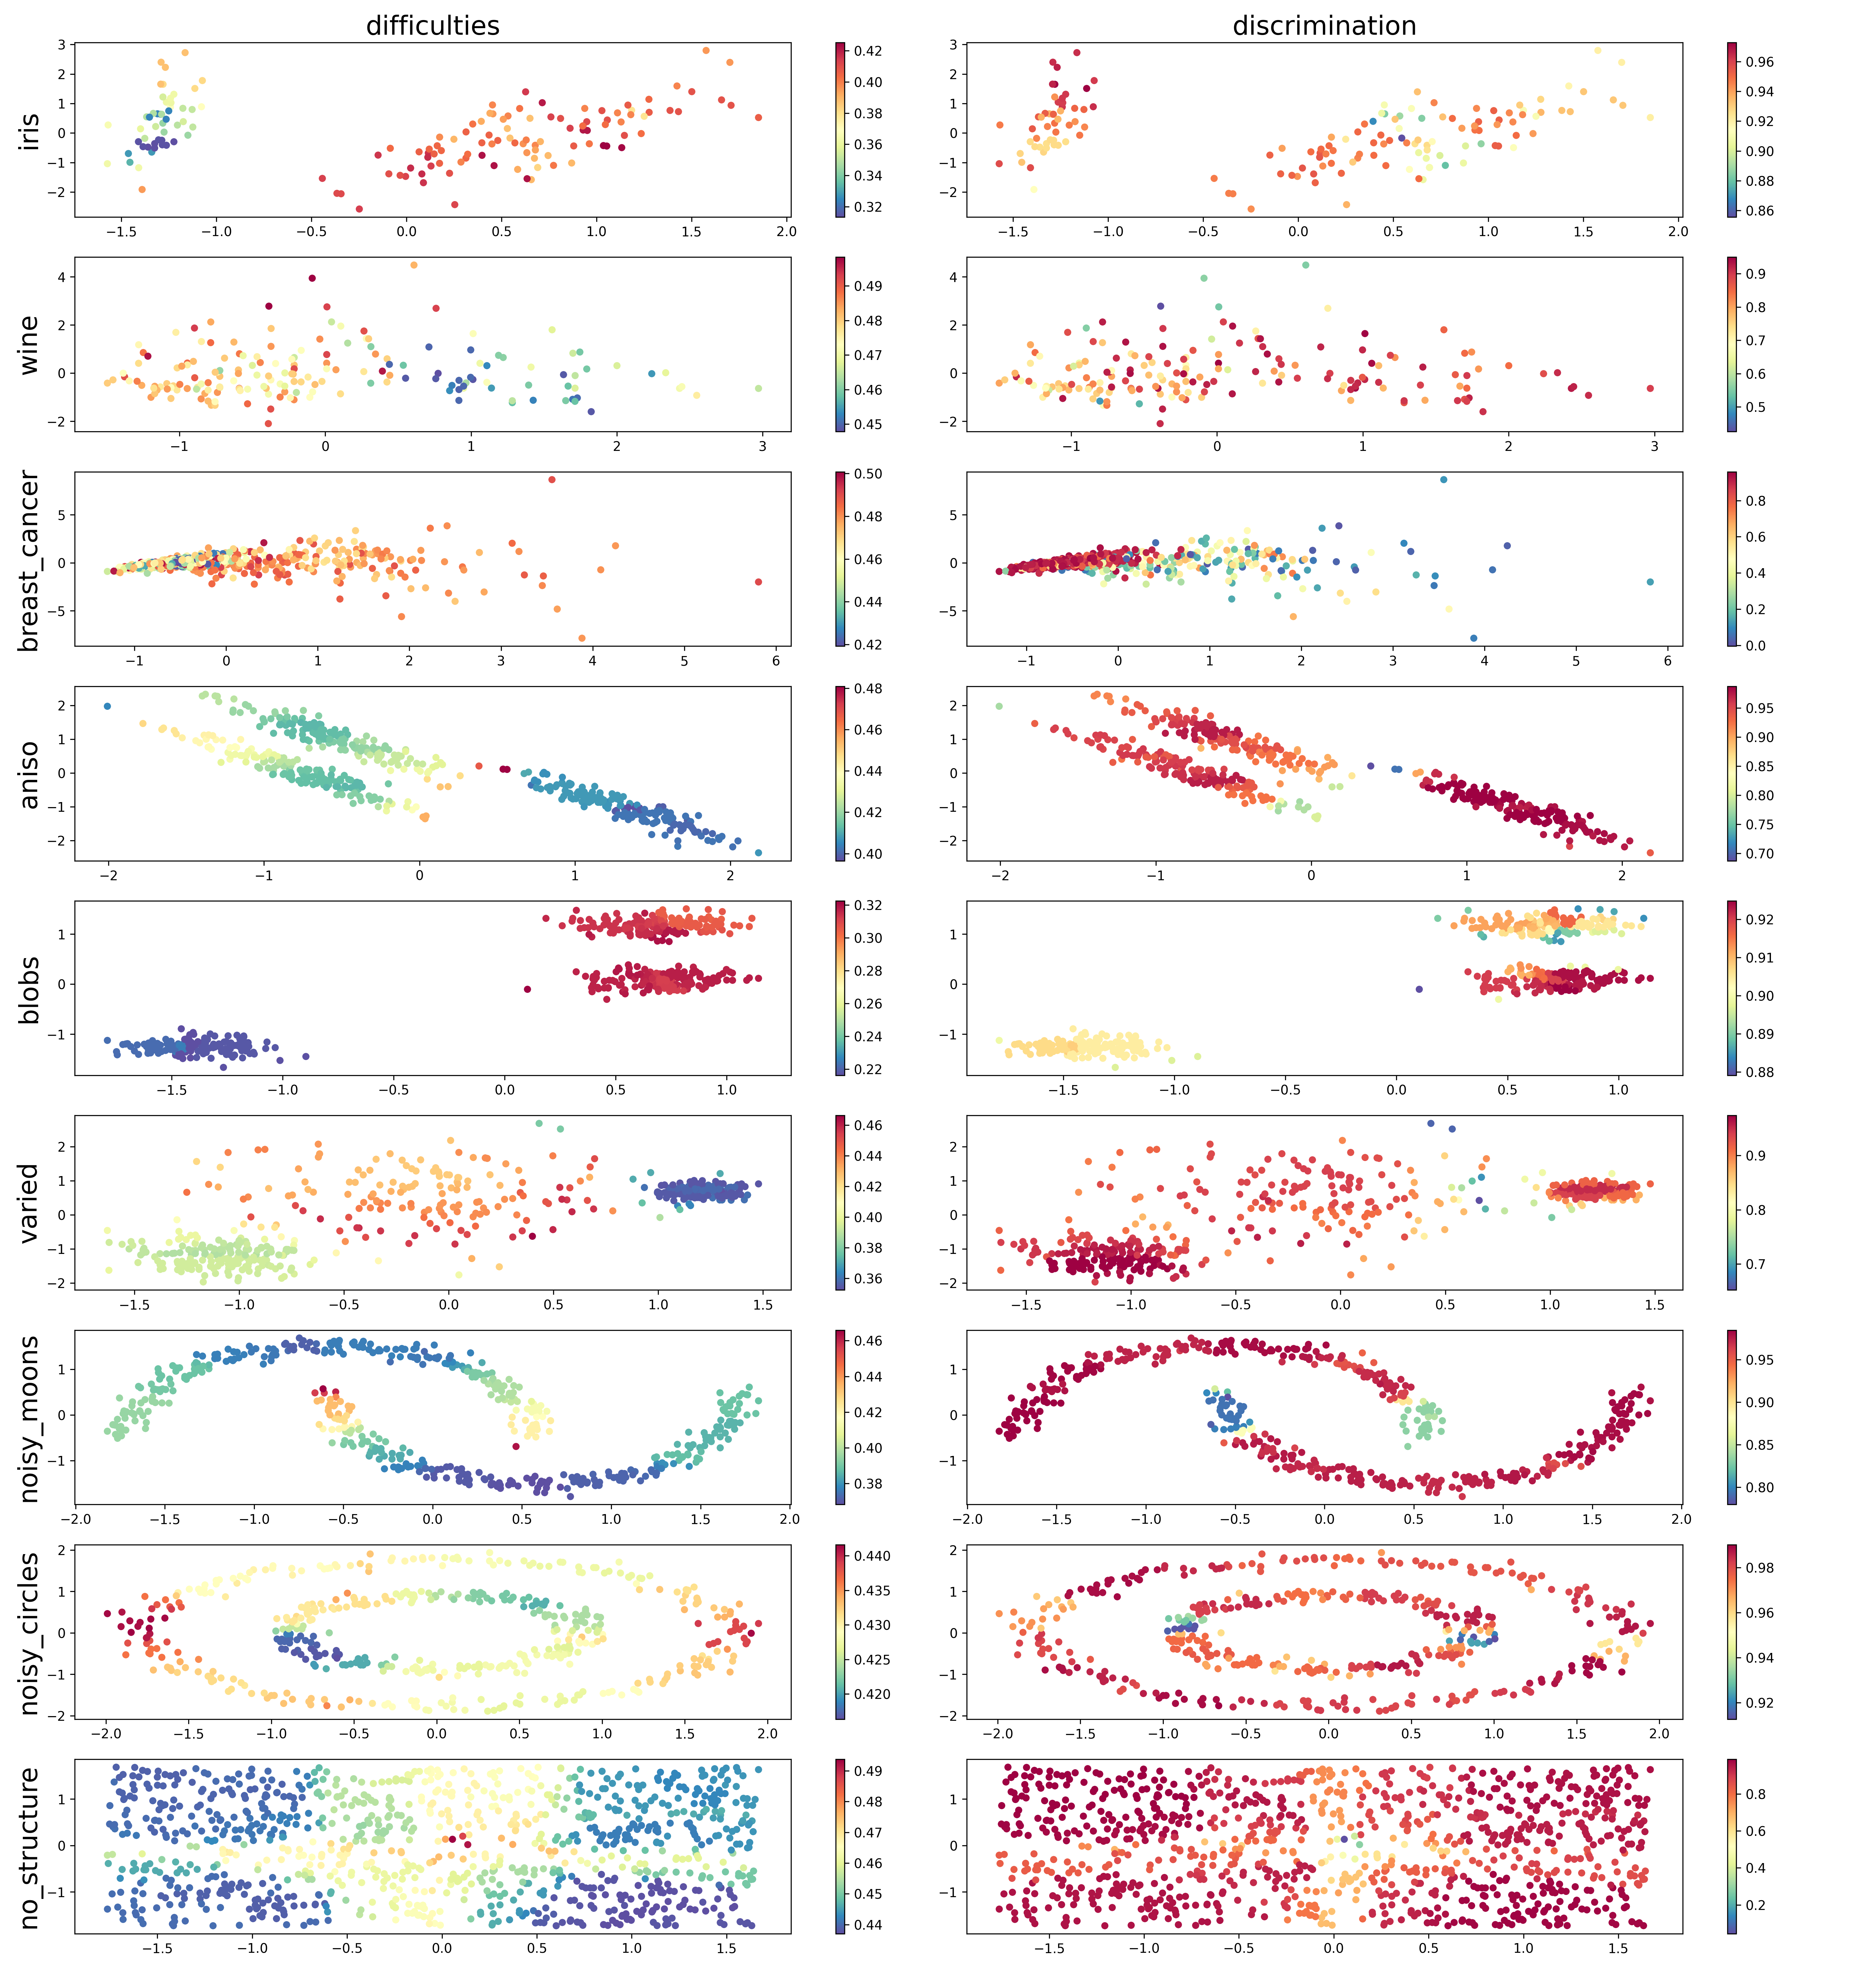
\includegraphics[width=\linewidth]{images/claire/random_n0_diff_disc_all.png}
\end{minipage}%
\caption{Dificuldades e discriminações estimadas para cada conjunto de dados (sem partições aleatórias).}
\end{figure}


\begin{figure}
\centering
\begin{minipage}{.41\textwidth}
  \centering
  \includegraphics[width=\linewidth]{images/claire/simulation_dataset.png}
\end{minipage}%
\caption{Habilidades estimadas para números crescentes de partições aleatórias no conjunto de modelos.}
\end{figure}

